\RequirePackage{fix-cm}
\documentclass{article}
% Anonymous review format. Official 2027 style replacement is pending;
% see templates/cpal/README.md for the authentic base and metadata adapter.
\usepackage{cpal_submission}

% --- Packages ---
\usepackage{xcolor}
\usepackage{amsmath,amsthm,amssymb}
\usepackage{bm}
\usepackage{derivative}
\usepackage{xurl}          % allow long bibliography URLs to wrap
\usepackage{hyperref}     % hyperlinks
\hypersetup{
    pdfauthor={},
    pdftitle={Prediction Risk After Observation Compression},
    colorlinks=true,
    linkcolor={blue!80!black},
    citecolor={green!50!black},
    urlcolor=blue
}
% \usepackage{cleveref}     % load after hyperref, avoid using this, will cause ref errors!
% \usepackage{thmtools}     % avoid using this

\usepackage{graphicx}
\usepackage{placeins}
\usepackage{array}
\usepackage{booktabs}
\graphicspath{{Code_CPAL/}}

% --- Theorem-like environments ---
\theoremstyle{plain} % italic text, bold heading
\newtheorem{theorem}{Theorem}[section]
\newtheorem{lemma}[theorem]{Lemma}
\newtheorem{proposition}[theorem]{Proposition}
\newtheorem{corollary}[theorem]{Corollary}
\newtheorem{claim}[theorem]{Claim}


\theoremstyle{definition} % upright text, bold heading
\newtheorem{definition}[theorem]{Definition}
\newtheorem{assumption}[theorem]{Assumption}
\newtheorem{example}[theorem]{Example}

\theoremstyle{definition} % upright remarks
\newtheorem{remark}{Remark}

% --- Cleveref naming customization ---
% \refname{assumption}{Assumption}{Assumptions}
% \refname{equation}{Eq.}{Eqs.}

%% useful math notations are defined here
\newcommand{\boldone}{\mathbf{1}}
\newcommand{\boldzero}{\mathbf{0}}
\usepackage{mathtools}
\DeclarePairedDelimiter\norm{\lVert}{\rVert}
\DeclarePairedDelimiter\fnorm{\lVert}{\rVert_{\rm{F}}}
\DeclarePairedDelimiter\opnorm{\lVert}{\rVert_{\rm{op}}}

\def\cbA{\check{\mathbold{A}}}
\def\cbK{\check{\mathbold{K}}}
\def\cbTheta{\check{\mathbold{\Theta}}}



\def\bUpsilon{\mathbold{\Upsilon}}
\def\tbUpsilon{\widetilde{\mathbold{\Upsilon}}}

\def\tx{{\tilde x}}
\def\tD{{\tilde D}}
\def\tF{{\tilde F}}


\def\tcalD{{\widetilde{\cal D}}}
\newcommand{\indep}{\perp\!\!\!\perp}


\def\tDelta{{\tilde \Delta}}
\def\defas{\stackrel{\text{\tiny def}}{=}}
\def\df{\hat{\mathsf{df}}}
\def\tdf{\tilde{\mathsf{df}}}

\def\Rem{{\mathrm{Rem}}}

\def\err{{\mathrm{Err}}}
\def\herr{\widehat{\mathrm{Err}}}

\def\Rembar{\overline{{\mathrm{Rem}}}}

\def\sign{{\rm sign}}
\def\var{{\rm var}}

\newcommand{\limd}{{\,\smash{\xrightarrow{\mathrm{d}}}}\,}
\newcommand{\limp}{{\,\smash{\xrightarrow{\mathrm{p}}}}\,}
\newcommand{\limas}{\,\smash{\xrightarrow{\mathrm{a.s.}}}\,}


\def\argmax{\mathop{\rm arg\, max}}
\def\argmin{\mathop{\rm arg\, min}}
\DeclareMathOperator{\prox}{prox}
\DeclareMathOperator{\soft}{soft}

\DeclareMathOperator{\trace}{Tr}
\DeclareMathOperator{\range}{range}
\DeclareMathOperator{\rank}{rank}
\let\vec\relax
\DeclareMathOperator{\vec}{\mathbf{vec}}
\DeclareMathOperator{\diag}{\mathbf{diag}}

\let\div\relax
\DeclareMathOperator{\div}{div}
\DeclareMathOperator{\supp}{supp}


\usepackage{xspace} 
\def\iid{i.i.d.\@\xspace}
\def\eg{e.g.\@\xspace}
\def\ie{i.e.\@\xspace}
\def\resp{resp.\@\xspace}

\def\I{{\mathbb{I}}}
\def\R{{\mathbb{R}}}
\def\E{{\mathbb{E}}}
\def\N{{\mathbb{N}}}
\def\P{{\mathbb{P}}}

\def\mathbold{\boldsymbol} %\def\mathbold{\mathbf}
\def\cal{\mathcal} %\def\mathbold{\mathbf}

\def\bvartheta{\mathbold{\vartheta}}

\def\ba{\mathbold{a}}\def\bfa{\mathbold{a}}\def\ahat{\widehat{a}}\def\atil{\widetilde{a}}
\def\hba{{\widehat{\ba}}}\def\tba{{\widetilde{\ba}}}\def\babar{{\overline{\ba}}}
\def\bA{\mathbold{A}}\def\calA{{\cal A}}\def\scrA{{\mathscr A}}\def\Ahat{\widehat{A}}\def\Atil{{\widetilde A}}
\def\hbA{\smash{\widehat{\mathbf A}}}\def\tbA{{\widetilde{\mathbf A}}}
\def\Ahati{{{\widehat A}_i}}\def\AhatJ{{{\widehat A}_{J,n}}}\def\Atili{{{\widetilde A}_i}}\def\AtilJ{{{\widetilde A}_{J,n}}}

\def\bb{\mathbold{b}}\def\bhat{\widehat{b}}\def\btil{\widetilde{b}}
\def\hbb{{\widehat{\bb}}}\def\tbb{{\widetilde{\bb}}}
\def\bB{\mathbold{B}}\def\calB{{\cal B}}\def\scrB{{\mathscr B}}\def\Bhat{\widehat{B}}\def\Btil{{\widetilde B}}
\def\hbB{{\widehat{\bB}}}\def\tbB{{\widetilde{\bB}}}

\def\bfc{\mathbold{c}}\def\bfC{\mathbold{C}}
\def\bc{\mathbold{c}}\def\chat{\widehat{c}}\def\ctil{\widetilde{c}}
\def\hbc{{\widehat{\bc}}}\def\tbc{{\widetilde{\bc}}}
\def\bC{\mathbold{C}}\def\calC{{\cal C}}\def\scrC{{\mathscr C}}\def\Chat{\widehat{C}}\def\Ctil{{\widetilde C}}
\def\hbC{{\widehat{\bC}}}\def\tbC{{\widetilde{\bC}}}

\def\bfd{\mathbold{d}}\def\dhat{\widehat{d}}\def\dtil{\widetilde{d}}
\def\hbd{{\widehat{\bd}}}\def\tbd{{\widetilde{\bd}}}
\def\bD{\mathbold{D}}\def\calD{{\cal D}}\def\scrD{{\mathscr D}}\def\Dhat{\widehat{D}}\def\Dtil{{\widetilde D}}
\def\hbD{{\widehat{\bD}}}\def\tbD{{\widetilde{\bD}}}
\def\bDbar{{\overline{\bD}}}

\def\bfe{\mathbold{e}}\def\ehat{\widehat{e}}\def\etil{\widetilde{e}}
\def\hbe{{\widehat{\bfe}}}\def\tbe{{\widetilde{\bfe}}}
\def\bE{\mathbold{E}}\def\calE{{\cal E}}\def\scrE{{\mathscr E}}\def\Ehat{\widehat{E}}\def\Etil{{\widetilde E}}
\def\hbE{{\widehat{\bE}}}\def\tbE{{\widetilde{\bE}}}

\def\bff{\mathbold{f}}\def\fhat{\widehat{f}}\def\hf{\widehat{f}}\def\ftil{\widetilde{f}}
\def\hbf{{\widehat{\bff}}}\def\tbf{{\widetilde{\bff}}}
\def\bF{\mathbold{F}}\def\calF{{\cal F}}\def\scrF{{\mathscr F}}\def\Fhat{\widehat{F}}\def\Ftil{{\widetilde F}}
\def\hbF{{\widehat{\bF}}}\def\tbF{{\widetilde{\bF}}}
\def\fphat{\widehat{f'_i}}\def\fbara{\bar{f}^{(1)}}\def\fbarb{\bar{f}^{(2)}}\def\fbarc{\bar{f}^{(3)}}

\def\bg{\mathbold{g}}\def\ghat{\widehat{g}}\def\gtil{\widetilde{g}}
\def\hbg{{\widehat{\bg}}}\def\tbg{{\widetilde{\bg}}}
\def\bG{\mathbold{G}}\def\calG{{\cal G}}\def\scrG{{\mathscr G}}\def\Ghat{\widehat{G}}\def\Gtil{{\widetilde G}}
\def\hbG{{\widehat{\bG}}}\def\tbG{{\widetilde{\bG}}}

\def\bh{\mathbold{h}}\def\hhat{\widehat{h}}\def\htil{\widetilde{h}}
\def\hbh{{\widehat{\bh}}}\def\tbh{{\widetilde{\bh}}}
\def\bH{\mathbold{H}}\def\calH{{\cal H}}\def\scrH{{\mathscr H}}\def\Hhat{\widehat{H}}\def\Htil{{\widetilde H}}
\def\hbH{{\widehat{\bH}}}\def\tbH{{\tilde{\bH}}}

\def\bi{\mathbold{i}}\def\ihat{\widehat{i}}\def\itil{\widetilde{i}}\def\ibar{{\overline i}}
\def\hbi{{\widehat{\bi}}}\def\tbi{{\widetilde{\bi}}}
\def\bI{\mathbold{I}}\def\hbI{{\widehat{\bI}}}\def\tbI{{\widetilde{\bI}}}
\def\calI{{\cal I}}\def\scrI{{\mathscr I}}\def\Ihat{\widehat{I}}\def\Itil{{\widetilde I}}\def\Ibar{{\overline I}}

\def\bj{\mathbold{j}}\def\jhat{\widehat{j}}\def\jtil{\widetilde{j}}\def\jbar{{\overline j}}
\def\hbj{{\widehat{\bj}}}\def\tbj{{\widetilde{\bj}}}
\def\bJ{\mathbold{J}}\def\hbJ{{\widehat{\bJ}}}\def\tbJ{{\widetilde{\bJ}}}
\def\calJ{{\cal J}}\def\scrJ{{\mathscr J}}\def\Jhat{\widehat{J}}\def\Jtil{{\widetilde J}}\def\Jbar{{\overline J}}

\def\bk{\mathbold{k}}\def\khat{\widehat{k}}\def\ktil{\widetilde{k}}\def\kbar{{\overline k}}
\def\hbk{{\widehat{\bk}}}\def\tbk{{\widetilde{\bk}}}
\def\bK{\mathbold{K}}\def\hbK{{\widehat{\bK}}}\def\tbK{{\widetilde{\bK}}}
\def\calK{{\cal K}}\def\scrK{{\mathscr K}}\def\Khat{\widehat{K}}\def\Ktil{{\widetilde K}}\def\Kbar{{\overline K}}

\def\bell{\mathbold{\ell}}\def\ellhat{\widehat{\ell}}\def\elltil{\widetilde{\ell}}\def\ellbar{{\overline \ell}}
\def\hbell{{\widehat{\bell}}}\def\tbell{{\widetilde{\bell}}}
\def\bL{\mathbold{L}}\def\hbL{{\widehat{\bL}}}\def\tbL{{\widetilde{\bL}}}
\def\calL{{\cal L}}\def\scrL{{\mathscr L}}\def\Lhat{\widehat{L}}\def\Ltil{{\widetilde L}}\def\Lbar{{\overline L}}
\def\dell{{\dot\ell}}\def\ddell{{\ddot\ell}}

\def\bbm{\mathbold{m}}\def\mhat{\widehat{m}}\def\mtil{\widetilde{m}}\def\mbar{{\overline m}}
\def\hbm{{\widehat{\bbm}}}\def\tbm{{\widetilde{\bbm}}}
\def\bM{\mathbold{M}}\def\hbM{{\widehat{\bM}}}\def\tbM{{\widetilde{\bM}}}
\def\calM{{\cal M}}\def\scrM{{\mathscr M}}\def\Mhat{\widehat{M}}\def\Mtil{{\widetilde M}}\def\Mbar{{\overline M}}

\def\bn{\mathbold{n}}\def\nhat{\widehat{n}}\def\ntil{\widetilde{n}}\def\nbar{{\overline n}}
\def\hbn{{\widehat{\bn}}}\def\tbn{{\widetilde{\bn}}}
\def\bN{\mathbold{N}}\def\hbN{{\widehat{\bN}}}\def\tbN{{\widetilde{\bN}}}
\def\calN{{\cal N}}\def\scrN{{\mathscr N}}\def\Nhat{\widehat{N}}\def\Ntil{{\widetilde N}}\def\Nbar{{\overline N}}

\def\bo{\mathbold{o}}\def\ohat{\widehat{o}}\def\otil{\widetilde{o}}\def\obar{{\overline o}}
\def\hbo{{\widehat{\bo}}}\def\tbo{{\widetilde{\bo}}}
\def\bO{\mathbold{O}}\def\hbO{{\widehat{\bO}}}\def\tbO{{\widetilde{\bO}}}
\def\calO{{\cal O}}\def\scrO{{\mathscr O}}\def\Ohat{\widehat{O}}\def\Otil{{\widetilde O}}\def\Obar{{\overline O}}

\def\bp{\mathbold{p}}\def\phat{\widehat{p}}\def\ptil{\widetilde{p}}\def\pbar{{\overline p}}
\def\hbp{{\widehat{\bp}}}\def\tbp{{\widetilde{\bp}}}
\def\bP{\mathbold{P}}\def\hbP{{\widehat{\bP}}}\def\tbP{{\widetilde{\bP}}}
\def\calP{{\cal P}}\def\scrP{{\mathscr P}}\def\Phat{\widehat{P}}\def\Ptil{{\widetilde P}}\def\Pbar{{\overline P}}

\def\bq{\mathbold{q}}\def\qhat{\widehat{q}}\def\qtil{\widetilde{q}}\def\qbar{{\overline q}}
\def\hbq{{\widehat{\bq}}}\def\tbq{{\widetilde{\bq}}}
\def\bQ{\mathbold{Q}}\def\hbQ{{\widehat{\bQ}}}\def\tbQ{{\widetilde{\bQ}}}
\def\calQ{{\cal Q}}\def\scrQ{{\mathscr Q}}\def\Qhat{\widehat{Q}}\def\Qtil{{\widetilde Q}}\def\Qbar{{\overline Q}}

\def\br{\mathbold{r}}\def\rhat{\widehat{r}}\def\rtil{\widetilde{r}}\def\rbar{{\overline r}}
\def\hbr{{\widehat{\br}}}\def\tbr{{\widetilde{\br}}}
\def\bR{\mathbold{R}}\def\hbR{{\widehat{\bR}}}\def\tbR{{\widetilde{\bR}}}
\def\calR{{\cal R}}\def\scrR{{\mathscr R}}\def\Rhat{\widehat{R}}\def\Rtil{{\widetilde R}}\def\Rbar{{\overline R}}

\def\bs{\mathbold{s}}\def\shat{\widehat{s}}\def\stil{\widetilde{s}}\def\sbar{{\overline s}}
\def\hbs{{\widehat{\bs}}}\def\tbs{{\widetilde{\bs}}}
\def\bS{\mathbold{S}}\def\hbS{{\widehat{\bS}}}\def\tbS{{\widetilde{\bS}}}
\def\calS{{\cal S}}\def\scrS{{\mathscr S}}\def\Shat{{\widehat{S}}}\def\Stil{{\widetilde S}}\def\Sbar{{\overline S}}

\def\bt{\mathbold{t}}\def\that{\widehat{t}}\def\ttil{\widetilde{t}}\def\tbar{{\overline t}}
\def\hbt{{\widehat{\bt}}}\def\tbt{{\widetilde{\bt}}}
\def\bT{\mathbold{T}}\def\hbT{{\widehat{\bT}}}\def\tbT{{\widetilde{\bT}}}
\def\calT{{\cal T}}\def\scrT{{\mathscr T}}\def\That{\widehat{T}}\def\Ttil{{\widetilde T}}\def\Tbar{{\overline T}}

\def\be{\mathbold{e}}

\def\bu{\mathbold{u}}\def\uhat{\widehat{u}}\def\util{\widetilde{u}}\def\ubar{{\overline u}}
\def\hbu{{\widehat{\bu}}}\def\tbu{{\widetilde{\bu}}}\def\bubar{{\overline{\bu}}}
\def\bU{\mathbold{U}}\def\hbU{{\widehat{\bU}}}\def\tbU{{\widetilde{\bU}}}
\def\calU{{\cal U}}\def\scrU{{\mathscr U}}\def\Uhat{\widehat{U}}\def\Util{{\widetilde U}}\def\Ubar{{\overline U}}

\def\bv{\mathbold{v}}\def\vhat{\widehat{v}}\def\vtil{\widetilde{v}}\def\vbar{{\overline v}}
\def\hbv{{\widehat{\bv}}}\def\tbv{{\widetilde{\bv}}}
\def\bV{\mathbold{V}}\def\hbV{{\widehat{\bV}}}\def\tbV{{\widetilde{\bV}}}
\def\calV{{\cal V}}\def\scrV{{\mathscr V}}\def\Vhat{\widehat{V}}\def\Vtil{{\widetilde V}}\def\Vbar{{\overline V}}

\def\bw{\mathbold{w}}\def\what{\widehat{w}}\def\wtil{\widetilde{w}}\def\wbar{{\overline w}}
\def\hbw{{\widehat{\bw}}}\def\tbw{{\widetilde{\bw}}}
\def\bW{\mathbold{W}}\def\hbW{{\widehat{\bW}}}\def\tbW{{\widetilde{\bW}}}
\def\calW{{\cal W}}\def\scrW{{\mathscr W}}\def\What{\widehat{W}}\def\Wtil{{\widetilde W}}\def\Wbar{{\overline W}}

\def\bx{\mathbold{x}}\def\xhat{\widehat{x}}\def\xtil{\widetilde{x}}\def\xbar{{\overline x}}\def\vbx{{\bf x}}
\def\hbx{{\widehat{\bx}}}\def\tbx{{\widetilde{\bx}}}\def\bxbar{{\overline \bx}}
\def\bX{\mathbold{X}}\def\hbX{{\widehat{\bX}}}\def\tbX{{\tilde{\bX}}}\def\bXbar{{\overline \bX}}
\def\calX{{\cal X}}\def\scrX{{\mathscr X}}\def\Xhat{\widehat{X}}\def\Xtil{{\widetilde X}}\def\Xbar{{\overline X}}

\def\by{\mathbold{y}}\def\yhat{\widehat{y}}\def\ytil{\widetilde{y}}\def\ybar{{\overline y}}\def\vby{{\bf y}}
\def\hby{{\widehat{\by}}}\def\tby{{\widetilde{\by}}}
\def\bY{\mathbold{Y}}\def\hbY{{\widehat{\bY}}}\def\tbY{{\widetilde{\bY}}}
\def\calY{{\cal Y}}\def\scrY{{\mathscr Y}}\def\Yhat{\widehat{Y}}\def\Ytil{{\widetilde Y}}\def\Ybar{{\overline Y}}

\def\bz{\mathbold{z}}\def\zhat{\widehat{z}}\def\ztil{\widetilde{z}}\def\zbar{{\overline z}}
\def\hbz{{\widehat{\bz}}}\def\tbz{{\widetilde{\bz}}}
\def\bZ{\mathbold{Z}}\def\hbZ{{\widehat{\bZ}}}\def\tbZ{{\widetilde{\bZ}}}
\def\calZ{{\cal Z}}\def\scrZ{{\mathscr Z}}\def\Zhat{\widehat{Z}}\def\Ztil{{\widetilde Z}}\def\Zbar{{\overline Z}}

%%% Greek
\def\balpha{\mathbold{\alpha}}\def\alphahat{\widehat{\alpha}}\def\halpha{\widehat{\alpha}}
\def\alphatil{\widetilde{\alpha}}\def\talpha{\widetilde{\alpha}}\def\alphabar{{\overline{\alpha}}}
\def\hbalpha{{\widehat{\balpha}}}\def\tbalpha{{\widetilde{\balpha}}}

\def\bbeta{\mathbold{\beta}}\def\betahat{\widehat{\beta}}\def\hbeta{\widehat{\beta}}
\def\betatil{\widetilde{\beta}}\def\tbeta{\widetilde{\beta}}\def\betabar{{\overline{\beta}}}
\def\hbbeta{\hat{\bbeta}{}}
\def\tbbeta{\tilde{\bbeta}}
\def\bbetabar{{\overline\bbeta}}

\def\bgamma{\mathbold{\gamma}}\def\gammahat{\widehat{\gamma}}\def\hgamma{\widehat{\gamma}}
\def\gammatil{\widetilde{\gamma}}\def\tgamma{\widetilde{\gamma}}\def\gammabar{{\overline{\gamma}}}
\def\hbgamma{{\widehat{\bgamma}}}\def\tbgamma{{\widetilde{\bgamma}}}\def\bgammabar{{\overline{\bgamma}}}

\def\bGamma{\mathbold{\Gamma}}\def\hbGamma{{\widehat{\bGamma}}}
\def\tbGamma{{\widetilde{\bGamma}}}\def\calGamma{{\cal \Gamma}}
\def\scrGamma{{\mathscr \Gamma}}\def\Gammahat{\widehat{\Gamma}}
\def\Gammatil{{\widetilde \Gamma}}\def\Gammabar{{\overline \Gamma}}

\def\bdelta{\mathbold{\delta}}\def\deltahat{\widehat{\delta}}\def\hdelta{\widehat{\delta}}
\def\deltatil{\widetilde{\delta}}\def\tdelta{\widetilde{\delta}}\def\deltabar{{\overline{\delta}}}
\def\hbdelta{{\widehat{\bdelta}}}\def\tbdelta{{\widetilde{\bdelta}}}

\def\bDelta{\mathbold{\Delta}}\def\hbDelta{{\widehat{\bDelta}}}
\def\tbDelta{{\widetilde{\bDelta}}}\def\calDelta{{\cal \Delta}}
\def\scrDelta{{\mathscr \Delta}}\def\Deltahat{\widehat{\Delta}}
\def\Deltatil{{\widetilde \Delta}}\def\Deltabar{{\overline \Delta}}

\def\ep{\varepsilon}\def\eps{\epsilon}\def\veps{\varepsilon}
\def\bep{ {\mathbold{\ep} }}
\def\ephat{\widehat{\ep}}\def\hep{\widehat{\ep}}
\def\eptil{\widetilde{\ep}}\def\tep{\widetilde{\ep}}\def\epbar{{\overline{\ep}}}
\def\hbep{{\widehat{\bep}}}\def\tbep{{\widetilde{\bep}}}

\def\bzeta{\mathbold{\zeta}}\def\zetahat{\widehat{\zeta}}\def\hzeta{\widehat{\zeta}}
\def\zetatil{\widetilde{\zeta}}\def\tzeta{\widetilde{\zeta}}\def\zetabar{{\overline{\zeta}}}
\def\hbzeta{{\widehat{\bzeta}}}\def\tbzeta{{\widetilde{\bzeta}}}

\def\bfeta{\mathbold{\eta}}\def\etahat{\widehat{\eta}}\def\heta{\widehat{\eta}}
\def\etatil{\widetilde{\eta}}\def\teta{\widetilde{\eta}}\def\etabar{{\overline{\eta}}}
\def\hbfeta{{\widehat{\bfeta}}}\def\tbfeta{{\widetilde{\bfeta}}}

\def\btheta{\mathbold{\theta}}\def\thetahat{\widehat{\theta}}\def\htheta{\widehat{\theta}}
\def\thetatil{\widetilde{\theta}}\def\ttheta{\widetilde{\theta}}\def\thetabar{{\overline{\theta}}}
\def\hbtheta{{\widehat{\btheta}}}\def\tbtheta{{\widetilde{\btheta}}}

\def\bTheta{\mathbold{\Theta}}\def\hbTheta{{\widehat{\bTheta}}}\def\bThetabar{{\overline \bTheta}}
\def\tbTheta{{\widetilde{\bTheta}}}\def\calTheta{{\cal \Theta}}
\def\scrTheta{{\mathscr \Theta}}\def\Thetahat{\widehat{\Theta}}
\def\Thetatil{{\widetilde \Theta}}\def\Thetabar{{\overline \Theta}}

\def\bkappa{\mathbold{\kappa}}\def\kappahat{\widehat{\kappa}}\def\hkappa{\widehat{\kappa}}
\def\kappatil{\widetilde{\kappa}}\def\tkappa{\widetilde{\kappa}}\def\kappabar{{\overline{\kappa}}}
\def\hbkappa{{\widehat{\bkappa}}}\def\tbkappa{{\widetilde{\bkappa}}}

\def\lam{\lambda}
\def\blam{\mathbold{\lam}}\def\lamhat{\widehat{\lam}}\def\hlam{\widehat{\lam}}
\def\lamtil{\widetilde{\lam}}\def\tlam{\widetilde{\lam}}\def\lambar{{\overline{\lam}}}
\def\hblam{{\widehat{\blam}}}\def\tblam{{\widetilde{\blam}}}

\def\blambda{\mathbold{\lambda}}\def\lambdahat{\widehat{\lambda}}\def\hlambda{\widehat{\lambda}}
\def\lambdatil{\widetilde{\lambda}}\def\tlambda{\widetilde{\lambda}}\def\lambdabar{{\overline{\lambda}}}
\def\hblambda{{\widehat{\blambda}}}\def\tblambda{{\widetilde{\blambda}}}

\def\bLambda{\mathbold{\Lambda}}\def\hbLambda{{\widehat{\bLambda}}}
\def\tbLambda{{\widetilde{\bLambda}}}\def\calLambda{{\cal \Lambda}}
\def\scrLambda{{\mathscr \Lambda}}\def\Lambdahat{\widehat{\Lambda}}
\def\Lambdatil{{\widetilde \Lambda}}\def\Lambdabar{{\overline \Lambda}}

\def\bmu{\mathbold{\mu}}\def\muhat{\widehat{\mu}}\def\hmu{\widehat{\mu}}
\def\mutil{\widetilde{\mu}}\def\tmu{\widetilde{\mu}}\def\mubar{{\overline{\mu}}}
\def\hbmu{{\widehat{\bmu}}}\def\tbmu{{\widetilde{\bmu}}}

\def\bnu{\mathbold{\nu}}\def\nuhat{\widehat{\nu}}\def\hnu{\widehat{\nu}}
\def\nutil{\widetilde{\nu}}\def\tnu{\widetilde{\nu}}\def\nubar{{\overline{\nu}}}
\def\hbnu{{\widehat{\bnu}}}\def\tbnu{{\widetilde{\bnu}}}

\def\bxi{\mathbold{\xi}}\def\xihat{\widehat{\xi}}\def\hxi{\widehat{\xi}}
\def\xitil{\widetilde{\xi}}\def\txi{\widetilde{\xi}}\def\xibar{{\overline{\xi}}}
\def\hbxi{{\widehat{\bxi}}}\def\tbxi{{\widetilde{\bxi}}}

\def\bXi{\mathbold{\Xi}}\def\hbXi{{\widehat{\bXi}}}
\def\tbXi{{\widetilde{\bXi}}}\def\calXi{{\cal \Xi}}
\def\scrXi{{\mathscr \Xi}}\def\Xihat{\widehat{\Xi}}
\def\Xitil{{\widetilde \Xi}}\def\Xibar{{\overline \Xi}}

\def\bpi{\mathbold{\pi}}\def\pihat{\widehat{\pi}}\def\hpi{\widehat{\pi}}
\def\pitil{\widetilde{\pi}}\def\tpi{\widetilde{\pi}}\def\pibar{{\overline{\pi}}}
\def\hbpi{{\widehat{\bpi}}}\def\tbpi{{\widetilde{\bpi}}}

\def\bPi{\mathbold{\Pi}}\def\hbPi{{\widehat{\bPi}}}
\def\tbPi{{\widetilde{\bPi}}}\def\calPi{{\cal \Pi}}
\def\scrPi{{\mathscr \Pi}}\def\Pihat{\widehat{\Pi}}
\def\Pitil{{\widetilde \Pi}}\def\Pibar{{\overline \Pi}}

\def\brho{\mathbold{\rho}}\def\rhohat{\widehat{\rho}}\def\hrho{\widehat{\rho}}
\def\rhotil{\widetilde{\rho}}\def\trho{\widetilde{\rho}}\def\rhobar{{\overline{\rho}}}
\def\hbrho{{\widehat{\brho}}}\def\tbrho{{\widetilde{\brho}}}

\def\bsigma{\mathbold{\sigma}}\def\sigmahat{\widehat{\sigma}}\def\hsigma{\widehat{\sigma}}
\def\sigmatil{\widetilde{\sigma}}\def\tsigma{\widetilde{\sigma}}\def\sigmabar{{\overline{\sigma}}}
\def\hbsigma{{\widehat{\bsigma}}}\def\tbsigma{{\widetilde{\bsigma}}}
\def\bsigmabar{{\overline\bsigma}}

\def\bSigma{\mathbold{\Sigma}}\def\hbSigma{{\widehat{\bSigma}}}
\def\tbSigma{{\widetilde{\bSigma}}}\def\calSigma{{\cal \Sigma}}
\def\scrSigma{{\mathscr \Sigma}}\def\Sigmahat{\widehat{\Sigma}}
\def\Sigmatil{{\widetilde \Sigma}}\def\Sigmabar{{\overline \Sigma}}
\def\bSigmabar{{\overline\bSigma}}

\def\btau{\mathbold{\tau}}\def\tauhat{\widehat{\tau}}\def\htau{\widehat{\tau}}
\def\tautil{\widetilde{\tau}}\def\ttau{\widetilde{\tau}}\def\taubar{{\overline{\tau}}}
\def\hbtau{{\widehat{\btau}}}\def\tbtau{{\widetilde{\btau}}}

\def\bphi{\mathbold{\phi}}\def\phihat{\widehat{\phi}}\def\hphi{\widehat{\phi}}
\def\phitil{\widetilde{\phi}}\def\tphi{\widetilde{\phi}}\def\phibar{{\overline{\phi}}}
\def\hbphi{{\widehat{\bphi}}}\def\tbphi{{\widetilde{\bphi}}}

\def\bPhi{\mathbold{\Phi}}\def\hbPhi{{\widehat{\bPhi}}}
\def\tbPhi{{\widetilde{\bPhi}}}\def\calPhi{{\cal \Phi}}
\def\scrPhi{{\mathscr \Phi}}\def\Phihat{\widehat{\Phi}}
\def\Phitil{{\widetilde \Phi}}\def\Phibar{{\overline \Phi}}

\def\bchi{\mathbold{\chi}}\def\chihat{\widehat{\chi}}\def\hchi{\widehat{\chi}}
\def\chitil{\widetilde{\chi}}\def\tchi{\widetilde{\chi}}\def\chibar{{\overline{\chi}}}
\def\hbchi{{\widehat{\bchi}}}\def\tbchi{{\widetilde{\bchi}}}

\def\bpsi{\mathbold{\psi}}\def\psihat{\widehat{\psi}}\def\hpsi{\widehat{\psi}}
\def\psitil{\widetilde{\psi}}\def\tpsi{\widetilde{\psi}}\def\psibar{{\overline{\psi}}}
\def\hbpsi{{\widehat{\bpsi}}}\def\tbpsi{{\widetilde{\bpsi}}}

\def\bPsi{\mathbold{\Psi}}\def\hbPsi{{\widehat{\bPsi}}}
\def\tbPsi{{\widetilde{\bPsi}}}\def\calPsi{{\cal \Psi}}
\def\scrPsi{{\mathscr \Psi}}\def\Psihat{\widehat{\Psi}}
\def\Psitil{{\widetilde \Psi}}\def\Psibar{{\overline \Psi}}

\def\bomega{\mathbold{\omega}}\def\omegahat{\widehat{\omega}}\def\homega{\widehat{\omega}}
\def\omegatil{\widetilde{\omega}}\def\tomega{\widetilde{\omega}}\def\omegabar{{\overline{\omega}}}
\def\hbomega{{\widehat{\bomega}}}\def\tbomega{{\widetilde{\bomega}}}

\def\bOmega{\mathbold{\Omega}}\def\hbOmega{{\widehat{\bOmega}}}
\def\tbOmega{{\widetilde{\bOmega}}}\def\calOmega{{\cal \Omega}}
\def\scrOmega{{\mathscr \Omega}}\def\Omegahat{\widehat{\Omega}}
\def\Omegatil{{\widetilde \Omega}}\def\Omegabar{{\overline \Omega}}

\newcommand{\MP}{\mathrm{MP}}
\newcommand{\SC}{\mathrm{SC}}
\newcommand{\st}{Stieltjes transform~}
\newcommand{\tv}{\tilde{v}}
\newcommand{\cv}{\check{v}}
\newcommand{\GCV}{{\text{GCV}}}
\newcommand{\init}{{\text{init}}}
\newcommand{\final}{{\text{final}}}
\newcommand{\tR}{\tilde{R}}
\newcommand{\hR}{\hat{R}}
\newcommand{\tc}{\tilde{c}}
\newcommand{\hSigma}{{\widehat{\Sigma}}}

\newcommand\gray[1]{{\color{gray} #1}}
\newcommand\kt[1]{{\color{red} #1}}
\newcommand\jw[1]{{\color{blue} #1}}
% Accepted revisions use the standard document formatting.
\DeclareRobustCommand{\rev}[1]{{#1}}
% Strip the template's heading prefix only from PDF bookmarks.
\pdfstringdefDisableCommands{\def\rev#1{#1}\def\hskip#1em.~~{}}

% --- Title info ---
\title{Prediction Risk After Observation Compression}
% Retained for a future preprint or accepted version; the review style masks it.
\author{Jiaying Weng \\
Department of Mathematical Sciences, Bentley University, USA \\
\texttt{jweng@bentley.edu}}
% Journal metadata retained here for the separate Statistica Sinica branch.
% MSC: primary 62J05; secondary 62F10, 62F12.
% Keywords: observation sketching; prediction risk; risk estimation;
% minimum-norm interpolation; generalized cross-validation.

% PaperFormalizer annotation macros
\RequirePackage{graphicx}
\definecolor{vsRed}{rgb}{0.80,0.00,0.00}
\definecolor{vsBlue}{rgb}{0.00,0.20,0.80}
\definecolor{vsNote}{rgb}{0.80,0.40,0.00}
\newcommand{\vsIndent}{1.5em}
\newcommand{\vsFirst}[2]{#1}
\newcommand{\vsSecond}[2]{#2}
\newcommand{\vsIfInner}{\ifhmode\ifinner\expandafter\expandafter\expandafter\vsFirst\else\expandafter\expandafter\expandafter\vsSecond\fi\else\expandafter\vsSecond\fi}
\newcommand{\vsBreak}{\ifhmode\ifinner\quad\else\unskip\par\fi\fi}
\makeatletter\newcommand{\vsEatCr}{\@ifnextchar\\{\vsGobbleCr}{}}\def\vsGobbleCr\\{\@ifstar{\@ifnextchar[\vsGobbleOpt{}}{\@ifnextchar[\vsGobbleOpt{}}}\def\vsGobbleOpt[#1]{}\makeatother
\newcommand{\vsBlock}[4]{\vsIfInner{\quad{\color{#1}#2\textbf{#3} #4}\quad}{\vsBreak\par\smallskip{\noindent\color{#1}#2\textbf{#3}\par\nopagebreak{\leftskip=\vsIndent\relax\parindent=0pt\noindent #4\par}}\smallskip\vsEatCr}}
\newcommand{\vsLine}{\vsBreak\noindent}
\newcommand{\vsLabel}[1]{}
\newcommand{\vsSub}{\vsIfInner{\ }{\vsBreak\noindent\hangindent=\vsIndent\hangafter=0\relax}}
\newcommand{\vsItem}[1]{\vsIfInner{\ #1~}{\vsBreak\noindent\hangindent=2.2em\hangafter=1\relax\makebox[2.2em][l]{#1}}}
\newcommand{\vsPar}{\vsIfInner{\quad}{\vsBreak}}
\newif\ifvsCheck
\newcommand{\vsFitIn}[2]{\vsIfInner{$#2$}{\[\displayindent=\dimexpr\displayindent+\leftskip\relax\displaywidth=\dimexpr\displaywidth-\leftskip-\rightskip\relax\sbox0{$\displaystyle #2$}#1\ifdim\wd0>\displaywidth\resizebox{\displaywidth}{!}{\usebox0}\else\usebox0\fi\]}}
\newif\ifvsTooWide
\newcommand{\vsFit}[1]{\vsFitIn{\ifvsCheck\ifdim\wd0>1.2\displaywidth\ifvsTooWide\else\global\vsTooWidetrue\xdef\vsTooWideMsg{Display too wide (\the\wd0, line \the\displaywidth): split it into rows (an aligned environment inside the display)}\fi\fi\fi}{#1}}
\newcommand{\vsCheckEnd}{\ifvsTooWide\errmessage{\vsTooWideMsg}\fi}
\newcommand{\vsDisplay}[1]{\vsFitIn{}{#1}}
\newcommand{\vsMathEnv}[2]{\vsIfInner{$#1$}{#2}}
\newcommand{\vsOriginal}[1]{\vsBlock{vsRed}{}{Original:}{#1}}
\newcommand{\vsCorrected}[1]{\vsBlock{vsBlue}{}{Revised:}{#1}}
\newcommand{\vsClarified}[1]{\vsBlock{vsBlue}{}{Clarified statement:}{#1}}
\newcommand{\vsNote}[1]{\vsBlock{vsNote}{\normalfont\small}{PaperFormalizer:}{#1}}
\newcommand{\vsReading}[1]{\vsBlock{vsNote}{\normalfont\small}{Clarification:}{#1}}
\newcommand{\vsReadingOwner}[1]{\vsBlock{vsNote}{\normalfont\small}{Clarification (author):}{#1}}
\newcommand{\vsReadingSymbol}[2]{\vsBlock{vsNote}{\normalfont\small}{Clarification (symbol #1):}{#2}}
\newcommand{\vsDetail}[1]{\vsBlock{vsNote}{\normalfont\small}{Proof detail:}{#1}}
\newcommand{\vsCondition}[1]{\vsBlock{vsNote}{\normalfont\small}{Bookkeeping condition:}{#1}}
\newcommand{\vsConditionOwner}[1]{\vsBlock{vsNote}{\normalfont\small}{Bookkeeping condition:}{#1}}
\newcommand{\vsProof}[1]{\vsBlock{vsBlue}{}{Revised proof (confirmed):}{#1}}
\newcommand{\vsStep}[1]{\vsBlock{vsRed}{}{Original:}{#1}}
\newcommand{\vsCorrectedStep}[1]{\vsBlock{vsBlue}{}{Revised:}{#1}}
\newcommand{\vsCorollary}[3]{\vsBlock{vsBlue}{}{Corollary of #2:}{#3}}
\newcommand{\vsProposedCorollary}[3]{\vsBlock{vsBlue}{}{Proposed corollary of #2 (awaiting your decision):}{#3}}
\newcommand{\vsSplitProposition}[3]{\vsBlock{vsBlue}{}{Proposition stated in #2:}{#3}}
\newcommand{\vsProposedSplitProposition}[3]{\vsBlock{vsBlue}{}{Proposed proposition stated in #2 (awaiting your decision):}{#3}}
\newcommand{\vsProposed}[1]{\vsBlock{vsBlue}{}{Proposed revision (awaiting your decision):}{#1}}
\newcommand{\vsProposedProof}[1]{\vsBlock{vsBlue}{}{Proof of the proposed statement:}{#1}}
\newcommand{\vsProposedStep}[1]{\vsBlock{vsBlue}{}{Revised (for the proposed statement):}{#1}}
\newcommand{\vsRewind}[1]{\vsBlock{vsNote}{\normalfont\small}{Proposed correction (awaiting your decision):}{#1}}
\newcommand{\vsCap}[1]{\vsBlock{vsNote}{\normalfont\small}{Revision not settled (awaiting your decision):}{#1}}
\makeatletter\@ifpackageloaded{ulem}{}{\usepackage[normalem]{ulem}}\makeatother
\newcommand{\vsStruck}[1]{{\color{vsRed}\sout{#1}}}
\newcommand{\vsStruckRed}[1]{{\color{vsRed}#1}}
\AtBeginDocument{\providecommand{\eqref}[1]{(\ref{#1})}\providecommand{\cref}{\ref}\providecommand{\Cref}{\ref}\providecommand{\autoref}{\ref}\providecommand{\citet}{\cite}\providecommand{\citep}{\cite}\providecommand{\citeauthor}{\cite}\providecommand{\citeyear}{\cite}}
\AtBeginDocument{\providecommand{\mathbb}{\mathbf}\providecommand{\mathfrak}{\mathrm}\providecommand{\lesssim}{\mathrel{\vcenter{\offinterlineskip\hbox{$<$}\hbox{$\sim$}}}}\providecommand{\gtrsim}{\mathrel{\vcenter{\offinterlineskip\hbox{$>$}\hbox{$\sim$}}}}}
% end of PaperFormalizer annotation macros
\begin{document}
\maketitle

\begin{abstract}
Observation sketching compresses \(n\) observations into \(m\) linear combinations while retaining all \(d\) features, thereby reducing the number of equations used for fitting. We study how to estimate the prediction risk of the resulting predictor, defined as its mean squared error on a new observation while treating the fitted predictor as fixed. We propose two estimators based on residual information from the original data. The first uses residual directions not captured by a data-independent sketch. Under Gaussian data, it is conditionally unbiased and yields confidence intervals for positive risk. The second applies an observable residual correction, whose accuracy is characterized using Gaussian--Stein identities and trace calibration. For Gaussian data and scaled orthogonal sketches, we derive a finite-sample comparison of the estimators' mean squared errors and identify a sketch-size threshold at which their relative accuracy reverses. Neither method requires refitting the model. We evaluate the estimators using row-sampling, weighted-Haar, and dense-Gaussian sketches under Gaussian and uniform errors. With Gaussian errors and \(m<n\), both estimators follow the mean true risk more closely than generalized cross-validation. For weighted-Haar and dense-Gaussian sketches, they are also closer to the mean true risk than Bellec's formula at larger sample sizes.
\end{abstract}

\section{Introduction}
\label{sec:intro}

Observation compression reduces the number of equations used to fit a predictor. In linear regression, an observation sketch replaces $n$ observations with $m$ linear combinations while retaining all $d$ features. When $m<n$, the resulting regression problem has fewer rows but the same feature coordinates. A sketch chosen independently of the data determines which combinations of the original observations enter this smaller fitting problem. While compression can make fitting more parsimonious, it can also change the prediction risk of the fitted model. This raises a natural question: after fitting a predictor from compressed data, how can we use the original observations to estimate its prediction risk on a new observation?

\vsReadingSymbol{$m$}{$m$ is the deterministic number of rows of the full-row-rank sketch $\bS\in\R^{m\times n}$, with $1\leq m\leq n$; it may vary with $n$ in asymptotic sequences. In Theorem~\ref{thm:cpal-complementary-law}: $m<n$, so the complementary subspace has positive dimension $n-m$; no restriction $d<m$ is imposed by the complementary-law construction. In Theorem~\ref{thm:cpal-risk-benchmarks}: The noninterpolating proportional regime has $d<m\leq n$ and $(d/n,m/n)\to(\gamma,\rho)$ with $0<\gamma<\rho\leq1$. In Theorem~\ref{thm:tight-frame-mse-comparison}, Theorem~\ref{thm:cpal-mse-comparison}: $d+3<m<n$. In Theorem~\ref{thm:cpal-mse-comparison}: $(d/n,m/n)\to(\gamma,\rho)$ with $0<\gamma<\rho<1$; the local crossover definition treats $\rho_n=m/n$ as continuous, while the actual sketch size remains integer. In Theorem~\ref{thm:cpal-corrected-accuracy}, Lemma~\ref{lem:dot-beta}, Lemma~\ref{lem:dot-r}, Lemma~\ref{lem:dot-rh}, Lemma~\ref{lem:dot-hxh}, Lemma~\ref{lem:dot-rxr}, Lemma~\ref{lem:dot-rxxr}, Lemma~\ref{lem:dot-hxxh}, Lemma~\ref{lem:opnorm-X-bound}, Lemma~\ref{lem:M-inverse-bound}, Lemma~\ref{lem:balanced-Stein-sufficient-conditions}, Lemma~\ref{lem:balanced-moment-bounds}, Proposition~\ref{prop:Stein-risk-from-moments}, Proposition~\ref{eq:Q-identity-Sigma}, Lemma~\ref{lem:balanced-remainder-bounds}, Lemma~\ref{lem:balanced-trace-Stein-bounds}, Lemma~\ref{lem:balanced-exceptional-weight}, Proposition~\ref{prop:trace-calibration-general}: The standing noninterpolating range is $1\leq d<m\leq n$, and for all sufficiently large $n$ the balanced-sketch dimension gap satisfies $m-d\geq\kappa n$ for a fixed $\kappa>0$.}

\vsReadingSymbol{$d$}{$d$ is the deterministic positive integer feature dimension at each sample size, and may vary with $n$. In Theorem~\ref{thm:cpal-risk-benchmarks}: The dimension sequence satisfies $(d/n,m/n)\to(\gamma,\rho)$ with $0<\gamma<\rho\leq1$. In Theorem~\ref{thm:cpal-mse-comparison}: The dimension sequence satisfies $d+3<m<n$ and $(d/n,m/n)\to(\gamma,\rho)$ with $0<\gamma<\rho<1$.}

% Our target is the prediction risk of this particular fitted model.
% The coefficients are held fixed, and the expectation is taken over an
% independent feature vector and response from the same population.
% This risk includes both noise in the new response and error in the
% fitted coefficients. It can vary across training samples and sketches.
% An estimate of the average performance of a sketching procedure therefore
% need not describe the risk of the predictor obtained in a particular
% application. We assess that realized fit without changing its coefficients.

A difficulty is that the training residuals reuse the responses that determined the fitted coefficients, so they cannot generally be treated as independent assessment errors. Row sampling provides a simple example of how to avoid this dependence: observations not selected for fitting can be used to evaluate the fitted predictor. Dense sketches are different because they can mix all $n$ observations, leaving no individual observations unused. Nevertheless, when $m<n$, the sketch leaves directions in the original observation space that are orthogonal to its rows. These directions do not enter the compressed fit, and residuals along them can therefore provide information about prediction risk. This observation reveals a tradeoff controlled by the sketch size: increasing $m$ provides more directions for fitting but leaves fewer directions for assessment.

Existing work on sketching has largely studied what is gained or lost in the fitting step. In numerical linear algebra, random projections and row sampling can approximate the full-data regression objective or coefficient vector by solving a smaller regression problem \citep{drineas2011faster}. The surveys of \citet{mahoney2011randomized} and \citet{woodruff2014sketching} describe the computational savings and matrix operations underlying these methods, while \citet{pilanci2016iterative} studied iterative sketches for obtaining accurate solutions to constrained least-squares problems. Statistical work has gone further by asking how compression affects estimation and prediction. \citet{ma2015statistical} analyzed the bias and variance of regression estimators based on statistical leverage-score sampling. \citet{raskutti2016statistical} distinguished residual efficiency from fixed-design prediction efficiency, showing that a good numerical approximation need not imply good statistical prediction. \citet{dobriban2019asymptotics} derived limiting efficiencies for parameter estimation and prediction under several sketch families when the sample size and feature dimension grow together, and \citet{chen2023sketched} studied prediction risk and sketch-size selection for unpenalized regression, including regimes in which downsampling improves generalization. Together, these results describe how the size and structure of a sketch affect the predictor obtained from compressed data. 
Here, we focus on how to estimate the risk of the particular predictor obtained from an observed dataset and sketch.

This question is closely related to the broader problem of estimating prediction error from the data used for fitting. Generalized cross-validation (GCV) adjusts training residual error for model complexity \citep{golub1979generalized}. More recently, \citet{bellec2023out} developed out-of-sample error estimates for regression with convex penalties under Gaussian features, and \citet{patil2022estimating} estimated the conditional prediction-error distribution for high-dimensional ridge regression. Results specific to subsampling and sketching have also appeared. For subsampled estimators, \citet{bellec2025corrected} developed corrected GCV and risk-estimation bounds; their full-data criterion for a single row-subsample fit that exactly matches the sampled responses agrees with the estimate based on unused observations. \citet{patil2024asymptotically} showed that ordinary GCV can be inconsistent for finite observation-sketch ensembles, including a single sketch, and described a correction using both sketched and unsketched information. These developments motivate a more direct question for observation sketching: what residual information remains after compression, and how accurately can it estimate the risk of the compressed-data predictor?

We answer this question in two ways. The first method uses residual directions orthogonal to the sketch rows, extending the idea of evaluating a row-sampled fit on unused observations to general observation sketches. The second uses the full-data residual but corrects for its dependence on the fitted coefficients. Both methods evaluate the same predictor fitted from the compressed data and require no refitting. They use the original observations, or quantities sufficient to compute the relevant residuals. The two approaches also use the available residual information differently, which allows us to study how their relative accuracy depends on the amount of compression.
% Assessment adds a computational cost to forming and solving the compressed regression problem.

Our main results characterize these two approaches. Under Gaussian features and errors, we first derive an exact conditional residual law for any linear predictor constructed only from the compressed data, provided that the independent sketch has linearly independent rows and $m<n$. This result gives a conditionally unbiased estimator of prediction risk and a confidence interval for positive risk. For least squares with $d<m$, we then derive an observable correction to the full-data residual, together with a reference based on the population feature covariance. Under the stated assumptions, their expected absolute errors are bounded by a constant times $n^{-1/2}$.
%This assumes Gaussian features, errors with uniformly controlled Gaussian tails, and \(m-d\) proportional to \(n\). The sketch’s observation weight matrix must have nonzero eigenvalues within fixed positive bounds after overall scale normalization.
For sketches with independent Gaussian entries, we further establish consistency under Gaussian features and errors and quantify the discrepancy between ordinary GCV and prediction risk when the dimensions grow proportionally. Finally, for scaled orthogonal sketches under Gaussian data, we obtain a finite-sample comparison of the mean squared errors of the two risk estimators and derive a limiting sketch-size threshold at which their relative accuracy changes.
% The analysis assumes Gaussian features and errors with positive error variance, orthogonal sketch rows of equal length, and \(d+3<m<n\).
These results show that compression determines not only the predictor being fitted but also the residual information available for assessing it. In particular, they clarify when that remaining information is sufficient for accurate risk estimation and how the sketch size affects the accuracy of different assessment methods.


\section{Compressed regression and prediction risk}
\label{sec:meth}

For $i=1,\ldots,n$, let
$y_i=\bx_i^\top\bbeta^*+\varepsilon_i$, with a fixed coefficient vector
$\bbeta^*\in\R^d$. The feature vectors are independent and identically
distributed, with mean zero and covariance $\bSigma$, whose eigenvalues
lie between fixed positive constants. The errors are independent and
identically distributed, independent of the features, with mean zero and
variance $\sigma^2$. Write
$\bX=(\bx_1,\ldots,\bx_n)^\top\in\R^{n\times d}$,
$\by=(y_1,\ldots,y_n)^\top$, and
$\bep=(\varepsilon_1,\ldots,\varepsilon_n)^\top$.
A sketch $\bS\in\R^{m\times n}$, $1\leq m\leq n$, is independent of the
data and has full row rank almost surely. The compressed data
$(\bS\bX,\bS\by,\bS)$ are then used to produce the fitted coefficients
$\hbbeta$. The corresponding fitted predictor maps a feature vector
$\bx$ to $\bx^\top\hbbeta$.

\vsReadingSymbol{$\bbeta^*$}{$\bbeta^*\in\R^d$ is the fixed coefficient parameter in the response model, with its value specified under the response law being used. In Lemma~\ref{lem:balanced-trace-Stein-bounds}, Proposition~\ref{prop:trace-calibration-general}: Under $\E_{\rm aux}$, $\bbeta^*=\boldzero$; the original response law retains its original coefficient parameter. In Lemma~\ref{lem:balanced-moment-bounds}: The additional fitted-coefficient moment bounds assume $\norm{\bSigma^{1/2}\bbeta^*}\leq B$; this restriction is not imposed for the coefficient-error and residual moment bounds.}

\vsReadingSymbol{$\bSigma$}{$\bSigma$ is the population feature covariance at each sample size, with $c_{\bSigma}\bI_d\preceq\bSigma\preceq C_{\bSigma}\bI_d$ for fixed constants $0<c_{\bSigma}\leq C_{\bSigma}<\infty$ independent of $n$.}

\vsReadingSymbol{$\sigma^2$}{$\sigma^2=\operatorname{Var}(\varepsilon_i)$ is the population noise variance in the original observation model. In Theorem~\ref{thm:cpal-risk-benchmarks}, Theorem~\ref{thm:tight-frame-mse-comparison}, Theorem~\ref{thm:cpal-mse-comparison}: $\sigma^2>0$.}

\vsReadingSymbol{$\bx_i$}{$\bx_i\in\R^d$, for $i\in\{1,\ldots,n\}$, is the feature vector of the $i$th original observation and the transpose of the $i$th row of $\bX$.}

\vsReadingSymbol{$\varepsilon_i$}{For $i\in\{1,\ldots,n\}$, $\varepsilon_i=y_i-\bx_i^\top\bbeta^*$ is the structural observation error and the $i$th coordinate of $\bep$.}

\vsReadingSymbol{$\by$}{$\by=(y_1,\ldots,y_n)^\top=\bX\bbeta^*+\bep$ is the response vector for the response law under consideration. In Lemma~\ref{lem:dot-beta}, Lemma~\ref{lem:dot-r}, Lemma~\ref{lem:dot-rh}, Lemma~\ref{lem:dot-hxh}, Lemma~\ref{lem:dot-rxr}, Lemma~\ref{lem:dot-rxxr}, Lemma~\ref{lem:dot-hxxh}: Under design differentiation, $\bep=\by-\bX\bbeta^*$ is held fixed, so $\by=\bZ\bSigma^{1/2}\bbeta^*+\bep$ varies with $\bZ$. In Lemma~\ref{lem:balanced-trace-Stein-bounds}, Proposition~\ref{prop:trace-calibration-general}: Under the auxiliary response law, use the auxiliary response $\by=\bep$ when recomputing response-dependent quantities.}

\vsReadingSymbol{$\bep$}{$\bep=(\varepsilon_1,\ldots,\varepsilon_n)^\top=\by-\bX\bbeta^*$ denotes structural noise rather than fitted residuals. In Lemma~\ref{lem:dot-beta}, Lemma~\ref{lem:dot-r}, Lemma~\ref{lem:dot-rh}, Lemma~\ref{lem:dot-hxh}, Lemma~\ref{lem:dot-rxr}, Lemma~\ref{lem:dot-rxxr}, Lemma~\ref{lem:dot-hxxh}, Lemma~\ref{lem:balanced-Stein-sufficient-conditions}, Lemma~\ref{lem:balanced-moment-bounds}, Proposition~\ref{prop:Stein-risk-from-moments}, Proposition~\ref{eq:Q-identity-Sigma}, Lemma~\ref{lem:balanced-remainder-bounds}, Lemma~\ref{lem:balanced-trace-Stein-bounds}, Lemma~\ref{lem:balanced-exceptional-weight}, Proposition~\ref{prop:trace-calibration-general}: Design derivatives are pathwise with $\bep$ held fixed, together with $\bS$, $\bSigma$, and $\bbeta^*$; consequently $\by=\bX\bbeta^*+\bep$ varies with the design. In Lemma~\ref{lem:Stein-remainders-from-moments}: The field is differentiated with respect to $\bZ$ conditional on $(\bS,\bep)$, so the structural-noise coordinates are held fixed.}

\vsReadingSymbol{$\bS$}{$\bS\in\R^{m\times n}$ is the observation sketch acting on the left of $(\bX,\by)$, with $1\leq m\leq n$. In Lemma~\ref{lem:dot-beta}, Lemma~\ref{lem:dot-r}, Lemma~\ref{lem:dot-rh}, Lemma~\ref{lem:dot-hxh}, Lemma~\ref{lem:dot-rxr}, Lemma~\ref{lem:dot-rxxr}, Lemma~\ref{lem:dot-hxxh}, Lemma~\ref{lem:opnorm-X-bound}, Lemma~\ref{lem:M-inverse-bound}, Lemma~\ref{lem:balanced-Stein-sufficient-conditions}, Lemma~\ref{lem:balanced-moment-bounds}, Proposition~\ref{prop:Stein-risk-from-moments}, Proposition~\ref{eq:Q-identity-Sigma}, Lemma~\ref{lem:balanced-remainder-bounds}, Lemma~\ref{lem:balanced-trace-Stein-bounds}, Lemma~\ref{lem:balanced-exceptional-weight}, Proposition~\ref{prop:trace-calibration-general}: $\bS$ denotes the normalized representative $\overline{\bS}:=\{n/\trace(\bA)\}^{1/2}\bS$ constructed from the original sketch, so the reused symbols satisfy $\trace(\bS^\top\bS)=n$. In Theorem~\ref{thm:cpal-corrected-accuracy}: The statement permits the original sketch scale; its balanced-sketch proof replaces the sketch by the trace-normalized representative, using invariance of the fit and corrected risk estimates. In Theorem~\ref{thm:cpal-risk-benchmarks}, Theorem~\ref{thm:tight-frame-mse-comparison}, Theorem~\ref{thm:cpal-mse-comparison}: $\bS$ retains its natural sketch scale; a scaled orthogonal sketch satisfies $\bS\bS^\top=c_n\bI_m$ with $c_n>0$.}

\vsReadingSymbol{$\hbbeta$}{$\hbbeta\in\R^d$ denotes the fitted coefficient vector produced using only $(\bS\bX,\bS\by,\bS)$, hence is $\calF_{\bS}$-measurable. In Theorem~\ref{thm:cpal-corrected-accuracy}, Theorem~\ref{thm:cpal-risk-benchmarks}, Theorem~\ref{thm:tight-frame-mse-comparison}, Theorem~\ref{thm:cpal-mse-comparison}, Lemma~\ref{lem:dot-beta}, Lemma~\ref{lem:dot-r}, Lemma~\ref{lem:dot-rh}, Lemma~\ref{lem:dot-hxh}, Lemma~\ref{lem:dot-rxr}, Lemma~\ref{lem:dot-rxxr}, Lemma~\ref{lem:dot-hxxh}, Lemma~\ref{lem:opnorm-X-bound}, Lemma~\ref{lem:M-inverse-bound}, Lemma~\ref{lem:balanced-Stein-sufficient-conditions}, Lemma~\ref{lem:balanced-moment-bounds}, Proposition~\ref{prop:Stein-risk-from-moments}, Proposition~\ref{eq:Q-identity-Sigma}, Lemma~\ref{lem:balanced-remainder-bounds}, Lemma~\ref{lem:balanced-trace-Stein-bounds}, Lemma~\ref{lem:balanced-exceptional-weight}, Proposition~\ref{prop:trace-calibration-general}: $\hbbeta$ denotes $\hbbeta_{\bS}=\bM^{-1}\bX^\top\bA\by$, the unique sketched least-squares fit, with $\bA=\bS^\top\bS$, $\bM=\bX^\top\bA\bX$, and $\rank(\bS\bX)=d$. In Lemma~\ref{lem:balanced-trace-Stein-bounds}, Proposition~\ref{prop:trace-calibration-general}: When evaluated under $\E_{\rm aux}$, $\hbbeta$ is recomputed by the same fitting construction using the auxiliary response, with $\bbeta^*=\boldzero$ and $\bep\sim\calN(\boldzero,\bI_n)$.}

Let $(\bx_{\rm new},y_{\rm new})$ be an independent observation from
the same model. Our goal is to estimate the prediction risk of the
fitted predictor:
\begin{align}
 R&:=\E[(y_{\rm new}-\bx_{\rm new}^\top\hbbeta)^2
             \mid\bX,\by,\bS]\notag\\
  &=\sigma^2+(\hbbeta-\bbeta^*)^\top\bSigma(\hbbeta-\bbeta^*).
 \label{eq:cpal-prediction-risk}
\end{align}
Here the expectation is over the new observation, while the fitted
predictor is held fixed. Thus, $R$ accounts for both noise in the new
response and error in the fitted coefficients, measured with respect to
the feature distribution. Since $\hbbeta$ depends on the observed data
and the sketch, $R$ can vary across training samples and sketches.
Gaussian design means $\bX=\bZ\bSigma^{1/2}$, where $\bZ$ has independent
standard Gaussian entries. \emph{Gaussian data} means Gaussian design
and Gaussian errors $\bep\sim\calN(\boldzero,\sigma^2\bI_n)$.

\vsReadingSymbol{$R$}{$R$ is the prediction risk of the realized fitted predictor, integrating only the independent new observation while holding the fitted coefficients fixed; it is a function of the training data and sketch rather than their averaged risk.}

We estimate this risk using the residuals on the original observations,
$\bu=\by-\bX\hbbeta$. To describe which parts of these residuals are
retained or left out by compression, define
\begin{align}
 \bF&=(\bS\bS^\top)^{-1/2}\bS,\qquad
 \bP_{\bS}=\bF^\top\bF,\qquad
 \bQ_{\bS}=\bI_n-\bP_{\bS}.
 \label{eq:cpal-observation-geometry}
\end{align}
The row-whitened sketch $\bF\in\R^{m\times n}$ has orthonormal rows, so
$\bF\bF^\top=\bI_m$ and its row space is the same as that of $\bS$.
Consequently, $\bP_{\bS}$ projects onto the directions retained by the
sketch, while $\bQ_{\bS}$ projects onto the directions perpendicular to
them. Their ranks are $m$ and $n-m$, respectively, and
$\bu=\bP_{\bS}\bu+\bQ_{\bS}\bu$ gives the corresponding orthogonal
decomposition of the residual. This decomposition will be the basis for
the risk estimators developed below. 
% Here and below, $\norm{\cdot}$ is
% the Euclidean norm.

\vsReadingSymbol{$\bu$}{Outside an explicit local smooth-field declaration, $\bu:=\by-\bX\hbbeta\in\R^n$ denotes the residual of the fitted predictor on the original observations. In Theorem~\ref{thm:cpal-corrected-accuracy}, Theorem~\ref{thm:cpal-risk-benchmarks}, Theorem~\ref{thm:tight-frame-mse-comparison}, Theorem~\ref{thm:cpal-mse-comparison}, Lemma~\ref{lem:dot-beta}, Lemma~\ref{lem:dot-r}, Lemma~\ref{lem:dot-rh}, Lemma~\ref{lem:dot-hxh}, Lemma~\ref{lem:dot-rxr}, Lemma~\ref{lem:dot-rxxr}, Lemma~\ref{lem:dot-hxxh}, Lemma~\ref{lem:M-inverse-bound}, Lemma~\ref{lem:balanced-Stein-sufficient-conditions}, Lemma~\ref{lem:balanced-moment-bounds}, Proposition~\ref{prop:Stein-risk-from-moments}, Proposition~\ref{eq:Q-identity-Sigma}, Lemma~\ref{lem:balanced-remainder-bounds}, Lemma~\ref{lem:balanced-trace-Stein-bounds}, Lemma~\ref{lem:balanced-exceptional-weight}, Proposition~\ref{prop:trace-calibration-general}: The fitted coefficient is sketched least squares, so $\bu=\by-\bX\hbbeta_{\bS}=\bep-\bZ\bq$, with response-dependent quantities recomputed whenever the auxiliary response construction is used. In Lemma~\ref{lem:normalized-Gaussian-Stein}, a result cited in the proof of Lemma~\ref{lem:normalized-Gaussian-Stein}: In the cited one-vector inequality, $\bu:\R^{n\times d}\to\R^n$ is a general smooth field satisfying $\norm{\bu}\leq1$, rather than the regression residual; the transposed version interchanges $n$ and $d$.}


\section{Risk assessment from the complementary subspace}
\label{sec:cpal-complementary-assessment}

When $m<n$, the complementary subspace contains $n-m$ directions that are not used for fitting. We use the residuals along these directions to define
\begin{align*}
 \widehat R_c=\frac{\norm{\bQ_{\bS}\bu}^2}{n-m}.
\end{align*}
The index $c$ stands for complementary, and the dependence on the sketch is left implicit. To study this estimator, condition on
$\calF_{\bS}=\sigma(\bS\bX,\bS\by,\bS)$, which contains the information used for fitting. A $\calF_{\bS}$-measurable coefficient vector therefore depends only on the compressed data. Under Gaussian data, the retained and complementary components are independent conditional on $\bS$. Conditioning on $\calF_{\bS}$ thus fixes the fitted predictor and its risk $R$, while the complementary data remain random. We write $\mathcal L(\bV\mid\calF_{\bS})$ for a conditional distribution and $\chi^2_\nu$ for the sum of squares of $\nu$ independent standard Gaussians.

\vsReadingSymbol{$\widehat R_c$}{$\widehat R_c=\norm{\bQ_{\bS}\bu}^2/(n-m)$ is defined for $m<n$ using the residual of the fitted predictor under consideration. In Theorem~\ref{thm:cpal-complementary-law}: The residual is $\bu=\by-\bX\hbbeta$ for any $\calF_{\bS}$-measurable coefficient vector $\hbbeta$, where $\calF_{\bS}=\sigma(\bS\bX,\bS\by,\bS)$. In Theorem~\ref{thm:tight-frame-mse-comparison}, Theorem~\ref{thm:cpal-mse-comparison}: The residual is $\bu=\by-\bX\hbbeta_{\bS}$ for the sketched least-squares fit.}

\begin{theorem}
\label{thm:cpal-complementary-law}
\label{thm:complementary-validation}
Under the model above with Gaussian data and $m<n$, any
$\calF_{\bS}$-measurable $\hbbeta\in\R^d$ satisfies
\begin{align}
 \mathcal L(\bQ_{\bS}\bu\mid\calF_{\bS})
 &=\calN(\boldzero,R\bQ_{\bS}),\notag\\
 \frac{(n-m)\widehat R_c}{R}\,\bigg|\,\calF_{\bS}
 &\sim\chi^2_{n-m}\quad\text{on }R>0.
 \label{eq:cpal-complementary-law}
\end{align}
Under this regular conditional law,
$\E[\widehat R_c\mid\calF_{\bS}]=R$ and
$\operatorname{Var}(\widehat R_c\mid\calF_{\bS})=2R^2/(n-m)$,
without requiring unconditional moments of $R$.
\end{theorem}\vsReading{On the almost-sure event $\rank(\bS)=m$, $(\bS\bS^\top)^{-1/2}$ denotes the unique symmetric positive definite square root of $(\bS\bS^\top)^{-1}$. (the reading of a definition this result uses)}

The theorem gives a direct interpretation of $\widehat R_c$. Given $\calF_{\bS}$, the $n-m$ residual coordinates in an orthonormal basis of the complementary subspace are independent Gaussians with variance $R$, so their mean square is an unbiased estimate of $R$. The chi-square law also gives a confidence interval. If $q_{\nu,p}$ denotes the $p$-quantile of $\chi^2_\nu$ and $0<\alpha<1$, then
\begin{align}
 \left[
 \frac{(n-m)\widehat R_c}{q_{n-m,1-\alpha/2}},
 \frac{(n-m)\widehat R_c}{q_{n-m,\alpha/2}}
 \right]
 \label{eq:cpal-risk-interval}
\end{align}
has conditional coverage $1-\alpha$ when $R>0$. For $R>0$, the conditional relative variance of $\widehat R_c$ is $2/(n-m)$; fewer complementary directions therefore give less precise assessment. For row sampling, this construction reduces to the familiar use of held-out observations: $\bQ_{\bS}\bu$ contains the residuals on the unsampled observations, with zeros elsewhere. In this case, conditional unbiasedness requires only the model's second-moment assumptions, while Gaussianity gives the chi-square law. For a dense sketch, individual observations need not be left out, but the complementary directions play the same role. When $m=n$, the complementary subspace disappears and $\widehat R_c$ is undefined.

The same conditional law also applies when the compressed responses are fit exactly. When $d>m$ and $\rank(\bS\bX)=m$, the minimum-norm fit
$\hbbeta_{m,\bS}:=\argmin\{\norm{\bbeta}:\bS\bX\bbeta=\bS\by\}$
interpolates the compressed equations. Here the index $m$ denotes minimum norm. Since interpolation gives
$\bS\bu=\boldzero$, the residual lies entirely in the complementary subspace, so $\bQ_{\bS}\bu=\bu$ and
$\widehat R_c=\norm{\bu}^2/(n-m)$.
For row sampling, this coincides with the single-subsample interpolating formula of \citet{bellec2025corrected}.

%-----


\section{Residual correction for \texorpdfstring{$d<m$}{d < m}}
\label{sec:underparameterized-transfer}

When $d<m$, least squares generally does not fit the compressed responses exactly, so the residual contains both complementary and retained components. The retained component reuses the data used for fitting and therefore requires a correction. Define sketched least squares by
\begin{align*}
 \hbbeta_{\bS}
 :=\argmin_{\bbeta}\norm{\bS(\by-\bX\bbeta)}^2
 =\bM^{-1}\bX^\top\bA\by,\quad
 \bA=\bS^\top\bS,\quad \bM=\bX^\top\bA\bX.
\end{align*}
We assume $\rank(\bS\bX)=d$, as holds almost surely under Gaussian design. Here $R$ denotes the prediction risk of $\hbbeta_{\bS}$, $\bA\in\R^{n\times n}$, and $\bM\in\R^{d\times d}$. Let $\bu=\by-\bX\hbbeta_{\bS}$ and $\br=\bA\bu$. Adding a multiple of $\br$ changes the retained residual while leaving its complementary component unchanged. The correction is determined by
\begin{align*}
 b_{\bA}&=\trace(\bA)
       -\trace(\bA\bX\bM^{-1}\bX^\top\bA),&
 t_{\bSigma}&=\trace(\bSigma\bM^{-1}),
\end{align*}
where $\trace$ denotes the sum of the diagonal entries and $b_{\bA}>0$ measures the sketch weight remaining after fitting. These quantities lead to two corrected risk estimators,
\begin{align*}
 \hR_u=\frac{\norm{\bu+t_{\bSigma}\br}^2}{n},
 \qquad
 \hR_o=\frac{\norm{\bu+(d/b_{\bA})\br}^2}{n}.
\end{align*}
The index $u$ denotes the unobservable version, which depends on the population covariance through $t_{\bSigma}$, while $o$ denotes the observable version based only on the data. When $\bSigma$ is known, $\hR_u$ provides a useful reference for studying the correction. The observable estimator replaces $t_{\bSigma}$ with the trace-calibrated ratio $d/b_{\bA}$. Both estimators are invariant to an overall rescaling of the sketch. The following result shows that this calibration preserves the accuracy of the population-covariance correction.

\vsReadingSymbol{$\hbbeta_{\bS}$}{$\hbbeta_{\bS}$ is the unique sketched least-squares coefficient vector on $\{\rank(\bS\bX)=d\}$, computed from the response under consideration. In Lemma~\ref{lem:balanced-trace-Stein-bounds}, Proposition~\ref{prop:trace-calibration-general}: Under $\E_{\rm aux}$ the fit is recomputed from the auxiliary response; under the original response law it is the original fit.}

\vsReadingSymbol{$\bA$}{$\bA=\bS^\top\bS$ is the positive-semidefinite sketch Gram matrix of rank $m$, using the same sketch representative as $\bS$. In Lemma~\ref{lem:dot-beta}, Lemma~\ref{lem:dot-r}, Lemma~\ref{lem:dot-rh}, Lemma~\ref{lem:dot-hxh}, Lemma~\ref{lem:dot-rxr}, Lemma~\ref{lem:dot-rxxr}, Lemma~\ref{lem:dot-hxxh}, Lemma~\ref{lem:opnorm-X-bound}, Lemma~\ref{lem:M-inverse-bound}, Lemma~\ref{lem:balanced-Stein-sufficient-conditions}, Lemma~\ref{lem:balanced-moment-bounds}, Lemma~\ref{lem:influence-from-moments}, Proposition~\ref{prop:Stein-risk-from-moments}, Proposition~\ref{eq:Q-identity-Sigma}, Lemma~\ref{lem:balanced-remainder-bounds}, Lemma~\ref{lem:balanced-trace-Stein-bounds}, Lemma~\ref{lem:balanced-exceptional-weight}, Proposition~\ref{prop:trace-calibration-general}: $\bA$ denotes the trace-normalized representative: relative to the original sketch Gram matrix, it is multiplied by $n/\trace(\bA)$, so the reused symbol satisfies $\trace(\bA)=n$. In Theorem~\ref{thm:cpal-corrected-accuracy}: The statement permits the original sketch scale and imposes its spectral condition on $n\bA/\trace(\bA)$; the balanced-sketch proof uses the trace-normalized representative. In Theorem~\ref{thm:cpal-risk-benchmarks}, Theorem~\ref{thm:tight-frame-mse-comparison}, Theorem~\ref{thm:cpal-mse-comparison}: $\bA$ retains the natural sketch scale; in the scaled orthogonal case $\bA=c_n\bP_{\bS}$.}

\vsReadingSymbol{$\bM$}{$\bM=\bX^\top\bA\bX=(\bS\bX)^\top(\bS\bX)$ is the design-dependent Gram matrix of the current sketch, positive definite on the domain $\rank(\bS\bX)=d$. In Lemma~\ref{lem:dot-beta}, Lemma~\ref{lem:dot-r}, Lemma~\ref{lem:dot-rh}, Lemma~\ref{lem:dot-hxh}, Lemma~\ref{lem:dot-rxr}, Lemma~\ref{lem:dot-rxxr}, Lemma~\ref{lem:dot-hxxh}, Lemma~\ref{lem:M-inverse-bound}, Lemma~\ref{lem:balanced-Stein-sufficient-conditions}, Lemma~\ref{lem:balanced-moment-bounds}, Lemma~\ref{lem:influence-from-moments}, Proposition~\ref{prop:Stein-risk-from-moments}, Proposition~\ref{eq:Q-identity-Sigma}, Lemma~\ref{lem:balanced-remainder-bounds}, Lemma~\ref{lem:balanced-trace-Stein-bounds}, Lemma~\ref{lem:balanced-exceptional-weight}, Proposition~\ref{prop:trace-calibration-general}: $\bM$ is formed from the trace-normalized sketch Gram matrix with $\trace(\bA)=n$; relative to the natural-scale sketch, it is multiplied by $n/\trace(\bS^\top\bS)$.}

\vsReadingSymbol{$\br$}{Outside an explicit generic-field declaration, $\br:=\bA\bu\in\R^n$ is the weighted residual at the current sketch scale, recomputed from the current response quantities. In Lemma~\ref{lem:dot-beta}, Lemma~\ref{lem:dot-r}, Lemma~\ref{lem:dot-rh}, Lemma~\ref{lem:dot-hxh}, Lemma~\ref{lem:dot-rxr}, Lemma~\ref{lem:dot-rxxr}, Lemma~\ref{lem:dot-hxxh}, Lemma~\ref{lem:M-inverse-bound}, Lemma~\ref{lem:balanced-Stein-sufficient-conditions}, Lemma~\ref{lem:balanced-moment-bounds}, Lemma~\ref{lem:influence-from-moments}, Proposition~\ref{prop:Stein-risk-from-moments}, Proposition~\ref{eq:Q-identity-Sigma}, Lemma~\ref{lem:balanced-remainder-bounds}, Lemma~\ref{lem:balanced-trace-Stein-bounds}, Lemma~\ref{lem:balanced-exceptional-weight}, Proposition~\ref{prop:trace-calibration-general}: The standing weighted residual is $\br=\bA(\bep-\bZ\bq)$ for the trace-normalized representative, with $\trace(\bA)=n$; for the unregularized sketched least-squares fit, $\bZ^\top\br=\boldzero$. In Lemma~\ref{lem:derivative-energy-from-inverse-moments}: $\br\in\R^n$ is a general random vector field participating in the assumed identity $\partial\bq/\partial z_{ij}=\bK\be_jr_i-\bL^\top\be_iq_j$; the weighted-residual construction and sketched normal equations are not imposed. In Theorem~\ref{thm:tight-frame-mse-comparison}, Theorem~\ref{thm:cpal-mse-comparison}: The weighted residual retains the natural scaled orthogonal sketch scale: $\br=c_n\bP_{\bS}\bu$ when $\bA=c_n\bP_{\bS}$.}

\vsReadingSymbol{$b_{\bA}$}{$b_{\bA}$ is the positive residual sketch mass computed from the current sketch Gram matrix $\bA$ and design $\bX$; it depends on $(\bX,\bS)$ and not on the response. In Lemma~\ref{lem:dot-beta}, Lemma~\ref{lem:dot-r}, Lemma~\ref{lem:dot-rh}, Lemma~\ref{lem:dot-hxh}, Lemma~\ref{lem:dot-rxr}, Lemma~\ref{lem:dot-rxxr}, Lemma~\ref{lem:dot-hxxh}, Lemma~\ref{lem:M-inverse-bound}, Lemma~\ref{lem:balanced-Stein-sufficient-conditions}, Lemma~\ref{lem:balanced-moment-bounds}, Lemma~\ref{lem:influence-from-moments}, Proposition~\ref{prop:Stein-risk-from-moments}, Proposition~\ref{eq:Q-identity-Sigma}, Lemma~\ref{lem:balanced-remainder-bounds}, Lemma~\ref{lem:balanced-trace-Stein-bounds}, Lemma~\ref{lem:balanced-exceptional-weight}, Proposition~\ref{prop:trace-calibration-general}: Use the trace-normalized sketch $\overline{\bS}=\{n/\trace(\bS^\top\bS)\}^{1/2}\bS$ and its Gram matrix; $b_{\bA}$ denotes the resulting normalized residual sketch mass, equal to $n/\trace(\bS^\top\bS)$ times the mass of the natural-scale sketch.}

\vsReadingSymbol{$t_{\bSigma}$}{$t_{\bSigma}:=\trace(\bSigma\bM^{-1})$ depends on the design, sketch and population covariance, is unchanged by replacing only the response law, and scales by $c^{-1}$ when $\bA$ is replaced by $c\bA$. In Lemma~\ref{lem:dot-beta}, Lemma~\ref{lem:dot-r}, Lemma~\ref{lem:dot-rh}, Lemma~\ref{lem:dot-hxh}, Lemma~\ref{lem:dot-rxr}, Lemma~\ref{lem:dot-rxxr}, Lemma~\ref{lem:dot-hxxh}, Lemma~\ref{lem:M-inverse-bound}, Lemma~\ref{lem:balanced-Stein-sufficient-conditions}, Lemma~\ref{lem:balanced-moment-bounds}, Lemma~\ref{lem:influence-from-moments}, Proposition~\ref{prop:Stein-risk-from-moments}, Proposition~\ref{eq:Q-identity-Sigma}, Lemma~\ref{lem:balanced-remainder-bounds}, Lemma~\ref{lem:balanced-trace-Stein-bounds}, Lemma~\ref{lem:balanced-exceptional-weight}, Proposition~\ref{prop:trace-calibration-general}: The standing balanced-sketch notation evaluates $t_{\bSigma}$ using the trace-normalized sketch, so $\trace(\bA)=n$ and $t_{\bSigma}=\trace((\bZ^\top\bA\bZ)^{-1})$. In Theorem~\ref{thm:tight-frame-mse-comparison}, Theorem~\ref{thm:cpal-mse-comparison}: The scaled orthogonal sketch retains its natural scale $\bA=c_n\bP_{\bS}$; in the rotated whitened coordinates, $c_nt_{\bSigma}=\trace((\bZ_1^\top\bZ_1)^{-1})$.}

\vsReadingSymbol{$b$}{$b:=b_{\bA}=\trace(\bA)-\trace(\bA\bX\bM^{-1}\bX^\top\bA)$ is the positive residual sketch mass, depending on $(\bX,\bS)$ and unchanged when only the response law is replaced. In Lemma~\ref{lem:dot-beta}, Lemma~\ref{lem:dot-r}, Lemma~\ref{lem:dot-rh}, Lemma~\ref{lem:dot-hxh}, Lemma~\ref{lem:dot-rxr}, Lemma~\ref{lem:dot-rxxr}, Lemma~\ref{lem:dot-hxxh}, Lemma~\ref{lem:M-inverse-bound}, Lemma~\ref{lem:balanced-Stein-sufficient-conditions}, Lemma~\ref{lem:balanced-moment-bounds}, Lemma~\ref{lem:influence-from-moments}, Proposition~\ref{prop:Stein-risk-from-moments}, Proposition~\ref{eq:Q-identity-Sigma}, Lemma~\ref{lem:balanced-remainder-bounds}, Lemma~\ref{lem:balanced-trace-Stein-bounds}, Lemma~\ref{lem:balanced-exceptional-weight}, Proposition~\ref{prop:trace-calibration-general}: The standing balanced-sketch notation uses the trace-normalized representative $\overline{\bA}=n\bA/\trace(\bA)$, reusing $b$ for $b_{\overline{\bA}}=nb_{\bA}/\trace(\bA)$.}

\begin{theorem}
\label{thm:cpal-corrected-accuracy}
\label{thm:R-obs-general}
\label{thm:R-sens-general}
Assume Gaussian design and uniformly sub-Gaussian errors, meaning that
their tails admit a uniform Gaussian bound. For all sufficiently large
$n$, suppose almost surely that the positive eigenvalues of
$n\bA/\trace(\bA)$ lie in $[c_-,c_+]$, with fixed
$0<c_-\leq c_+<\infty$, and $m-d\geq\kappa n$ for a fixed $\kappa>0$.
Under the model conditions of Section~\ref{sec:meth}, a constant $C$
independent of $n$ satisfies
\begin{align}
 \max\{\E|\hR_o-R|,\E|\hR_u-R|\}\leq Cn^{-1/2}.
 \label{eq:cpal-corrected-accuracy}
\end{align}
\end{theorem}\vsReading{There exists a deterministic $K_\varepsilon<\infty$, independent of $n$, such that $\sup_n\norm{\varepsilon_1}_{\psi_2}\leq K_\varepsilon$, where $\norm{W}_{\psi_2}:=\inf\{t>0:\E\exp(W^2/t^2)\leq2\}$. (the reading of one of its hypotheses)}\vsReading{There exists a deterministic $n_0\geq1$ such that, for every $n\geq n_0$, almost surely every positive eigenvalue of $n\bA/\trace(\bA)$ belongs to $[c_-,c_+]$ and $m-d\geq\kappa n$, with $c_-,c_+,\kappa$ deterministic and independent of $n$. (the reading of one of its hypotheses)}\vsReadingSymbol{$c_-$}{$c_-$ is a strictly positive deterministic constant independent of $n$, with $c_-\leq c_+<\infty$, such that every positive eigenvalue of $n\bA/\trace(\bA)$ is at least $c_-$ almost surely for every sufficiently large $n$.}\vsReadingSymbol{$c_+$}{$c_+$ is a finite deterministic constant independent of $n$, with $0<c_-\leq c_+$, such that every positive eigenvalue of $n\bA/\trace(\bA)$ is at most $c_+$ almost surely for every sufficiently large $n$.}\vsReadingSymbol{$\kappa$}{$\kappa>0$ is a deterministic constant independent of $n$ such that $m-d\geq\kappa n$ for every sufficiently large $n$.}

Thus, both the population-covariance and observable corrections estimate $R$ with expected absolute error of order $n^{-1/2}$ under the stated conditions. Row sampling and reweightings of orthonormal sketch rows with weights bounded above and away from zero satisfy the spectral condition after normalization.

\subsection{Sketch geometry and risk benchmarks}

The form of the observable correction becomes especially transparent when the sketch has orthonormal rows.
A \emph{scaled orthogonal sketch} satisfies $\bS\bS^\top=c_n\bI_m$ for $c_n>0$; equivalently, $c_n^{-1/2}\bS$ has orthonormal rows. In this case, $\bA=c_n\bP_{\bS}$, $b_{\bA}=c_n(m-d)$, and
\begin{align}
 \hR_o=\frac{\norm{\bQ_{\bS}\bu}^2}{n}
       +\left(\frac{m}{m-d}\right)^2
        \frac{\norm{\bP_{\bS}\bu}^2}{n}.
 \label{eq:cpal-tight-frame-correction}
\end{align}
Thus, $\hR_o$ leaves the complementary residual unchanged and rescales only the retained residual. This distinction is important because the retained component is the part that reuses the fitting data. Although row whitening gives orthonormal rows for any full-row-rank sketch, replacing $\bS$ by $\bF$ can change the least-squares weights and hence the fitted predictor; only the interpolation constraints are preserved.

For comparison, GCV treats the residual differently: it rescales the entire full-data residual according to the trace $d$ of the fitted-value map,
\begin{align*}
 \hR_{\GCV}=\frac{\norm{\bu}^2/n}{(1-d/n)^2}.
\end{align*}
We compare scaled orthogonal sketches with dense Gaussian sketches, whose independent entries satisfy $S_{ki}\sim\calN(0,1/m)$. The latter require separate analysis because the preceding theorem's almost-sure spectral bounds do not apply. In the \emph{noninterpolating proportional regime}, $(\gamma_n,\rho_n):=(d/n,m/n)\to(\gamma,\rho)$ with $0<\gamma<\rho\leq1$. Write $\limp$ for convergence in probability.

\vsReadingSymbol{$\gamma_n$}{$\gamma_n=d/n$ is the deterministic dimension ratio along the sequence of sample sizes, with $d$ allowed to vary with $n$. In Theorem~\ref{thm:cpal-risk-benchmarks}: $(\gamma_n,\rho_n)\to(\gamma,\rho)$ with $0<\gamma<\rho\leq1$. In Theorem~\ref{thm:cpal-mse-comparison}: $(\gamma_n,\rho_n)\to(\gamma,\rho)$ with $0<\gamma<\rho<1$; the additional local-crossover conclusion assumes that $\gamma_n$ stays in a compact subset of $(0,1)$.}

\vsReadingSymbol{$\rho_n$}{$\rho_n=m/n$ is the deterministic sketch-size ratio along the sequence of sample sizes, with integer $1\leq m\leq n$ for actual sketches. In Theorem~\ref{thm:cpal-risk-benchmarks}: $(\gamma_n,\rho_n)\to(\gamma,\rho)$ with $0<\gamma<\rho\leq1$. In Theorem~\ref{thm:cpal-mse-comparison}: $(\gamma_n,\rho_n)\to(\gamma,\rho)$ with $0<\gamma<\rho<1$; in defining $\rho_n^{\#}$, $\rho_n$ is continuously extended and $m=n\rho_n$ need not be an integer.}

\vsReadingSymbol{$\gamma$}{$\gamma=\lim_{n\to\infty}d/n$ is the deterministic limiting feature-to-sample ratio, with $0<\gamma<1$. In Theorem~\ref{thm:cpal-risk-benchmarks}: The joint limiting ratios satisfy $0<\gamma<\rho\leq1$. In Theorem~\ref{thm:cpal-mse-comparison}: The joint limiting ratios satisfy $0<\gamma<\rho<1$.}

\vsReadingSymbol{$\rho$}{$\rho=\lim_{n\to\infty}\rho_n=\lim_{n\to\infty}m/n$ is a limiting sketch proportion satisfying $\gamma<\rho\leq1$. In Theorem~\ref{thm:cpal-mse-comparison}: $\rho<1$.}

\begin{theorem}
\label{thm:cpal-risk-benchmarks}
Under Gaussian data with $\sigma^2>0$ and this regime,
$R,\hR_u,\hR_o\limp\calR_j$ and $\hR_{\GCV}-R\limp\Delta_j$, where
$j$ identifies the sketch family:
\begin{align}
 \calR_{\rm SO}&=\frac{\sigma^2\rho}{\rho-\gamma},&
 \Delta_{\rm SO}&=
 \frac{\sigma^2\gamma^2(1-\rho)}
 {(\rho-\gamma)(1-\gamma)^2},\notag\\
 \calR_{\rm G}&=\sigma^2\left\{\frac1{1-\gamma}
                    +\frac{\gamma}{\rho-\gamma}\right\},&
 \Delta_{\rm G}&=\frac{\sigma^2\gamma^2}
 {(1-\gamma)(\rho-\gamma)}.
 \label{eq:cpal-risk-benchmarks}
\end{align}
Here SO denotes scaled orthogonal sketches and G denotes dense Gaussian sketches
with the stated entry law.
\end{theorem}

The limits $\calR_{\rm SO}$ and $\calR_{\rm G}$ agree with earlier sketch-risk benchmarks \citep{dobriban2019asymptotics,chen2023sketched}. The theorem also shows a difference between the two sketch families that is not visible from sketch size alone. At $\rho=1$, GCV's limiting gap is zero for scaled orthogonal sketches and positive for dense Gaussian sketches.

\subsection{Comparing estimation accuracy}

The preceding results establish consistency and characterize large-sample risk, but they do not determine which of the two proposed estimators is more accurate. We therefore compare $\widehat R_c$ and $\hR_o$ as estimates of the same fitted predictor's risk. For a risk estimate $T$, define its mean squared estimation error (MSE) as $\operatorname{MSE}(T)=\E[(T-R)^2]$, where the expectation averages over the training data and sketch randomness. For $d+3<m<n$, set $k=m-d$ and $q=n-m$, and define
\begin{align*}
   e_{m,d}&:=\frac{(m-1)(m-3)}{(k-1)(k-3)}, \notag\\
   a_{m,d}&:=\frac{2m^2}{k^3}
     +\frac{2d(m-1)}{(k-1)^2(k-3)}
     +\frac{d^2}{k^2(k-1)^2}.
\end{align*}

\vsReadingSymbol{$k$}{$k$ is a deterministic integer parameter bound by its local definition or quantifier. In Theorem~\ref{thm:tight-frame-mse-comparison}, Theorem~\ref{thm:cpal-mse-comparison}: In the finite-MSE expressions, $k=m-d>3$ and may vary with $n$. In Theorem~\ref{thm:cpal-complementary-law}: In the proof, $k=n-m>0$ is the rank of $\bQ_{\bS}$ and the complementary chi-square degrees of freedom. In Lemma~\ref{lem:opnorm-X-bound}, Lemma~\ref{lem:M-inverse-bound}, Lemma~\ref{lem:balanced-Stein-sufficient-conditions}, Lemma~\ref{lem:balanced-moment-bounds}, Lemma~\ref{lem:balanced-remainder-bounds}: In moment bounds, $k\geq1$ is an arbitrary fixed integer moment order, independent of $n$, rather than a dimension difference. In Theorem~\ref{thm:cpal-corrected-accuracy}: The proof's invocation of a moment bound at $k=1$ uses $k$ as moment order. In Lemma~\ref{lem:Stein-remainders-from-moments}: In the proof's rowwise derivative and covariance calculations, $k$ indexes a design row, with $1\leq k\leq n$ and $k\ne i$ where stated. In another result of the paper: $k$ is a locally bound design-row index, with $1\leq k\leq n$ and $k\ne i$.}

\vsReadingSymbol{$e_{m,d}$}{$e_{m,d}$ is the deterministic dimension-dependent coefficient defined for integer dimensions $1\leq d$ and $d+3<m<n$, using $k=m-d$.}

\vsReadingSymbol{$a_{m,d}$}{$a_{m,d}$ is the deterministic dimension-dependent coefficient defined for integer dimensions $1\leq d$ and $d+3<m<n$, using $k=m-d$.}

\vsReadingSymbol{$T$}{$T$ is local notation for a real-valued random quantity whose interpretation is specified in its surrounding definition. In Theorem~\ref{thm:tight-frame-mse-comparison}, Theorem~\ref{thm:cpal-mse-comparison}: $T$ denotes a risk estimate of the same fitted predictor's risk $R$, and $\operatorname{MSE}(T)=\E[(T-R)^2]$ averages over training data and sketch randomness. In Theorem~\ref{thm:cpal-risk-benchmarks}: In the dense Gaussian proof, $T\sim\chi^2_{n-d}$ is an auxiliary variable independent of $J,V,U,B$, introduced for marginal distributional representations of residual statistics.}

\begin{theorem}
\label{thm:tight-frame-mse-comparison}
Under the model of Section~\ref{sec:meth}, suppose Gaussian data,
$\sigma^2>0$, a scaled orthogonal sketch, and $1\leq d$ with $d+3<m<n$.
The mean squared errors are
\begin{align}
   \operatorname{MSE}(\widehat R_c)
   &=\frac{2\sigma^4e_{m,d}}q, \notag\\
   \operatorname{MSE}(\hR_o)&=
   \frac{\sigma^4}{n^2}\{2qe_{m,d}+m^2a_{m,d}\}.
   \label{eq:tight-frame-exact-mse-comparison}
\end{align}
The corrected risk estimate has smaller MSE exactly when
\begin{align}
   q^2+\frac{m^2q\,a_{m,d}}{2e_{m,d}}<n^2.
   \label{eq:tight-frame-finite-mse-rule}
\end{align}
Reversing the inequality favors the complementary risk estimate; equality
gives equal MSE.
\end{theorem}

The finite-sample comparison depends on $n$, $m$, and $d$. In the proportional regime, however, it simplifies to a threshold involving only the limiting dimension ratios. Define
\begin{align*}
 \rho_*(\gamma)=\frac{3\gamma}{1+2\gamma}.
\end{align*}
Let $\rho_n^{\#}$ denote the local continuous solution of
$\operatorname{MSE}(\hR_o)=\operatorname{MSE}(\widehat R_c)$ near
$\rho_*(\gamma_n)$, using the finite-sample expressions in
\eqref{eq:tight-frame-exact-mse-comparison}.
The finite ratio $\rho_n=m/n$ is treated as continuous for this definition.

\vsReadingSymbol{$\rho_n^{\#}$}{$\rho_n^{\#}$ is a deterministic local root near $\rho_*(d/n)$ of the finite-sample MSE equality after continuously extending $m=n\rho_n$; it need not correspond to an integer sketch size.}

\begin{theorem}
\label{thm:cpal-mse-comparison}
\label{thm:tight-frame-asymptotic-mse-threshold}
For Gaussian data with $\sigma^2>0$, a scaled orthogonal sketch, and
$d+3<m<n$, suppose $(\gamma_n,\rho_n)\to(\gamma,\rho)$ with
$0<\gamma<\rho<1$.
For sufficiently large $n$, $\widehat R_c$ has smaller MSE if
$\rho<\rho_*(\gamma)$, and $\hR_o$ has smaller MSE if
$\rho>\rho_*(\gamma)$. At equality, their MSE ratio tends to one.
If $\gamma_n$ stays in a compact subset of $(0,1)$, the local
continuous crossover exists uniquely for sufficiently large $n$ and
\begin{align}
 \rho_n^{\#}
 =\rho_*(\gamma_n)-\frac{5}{12n}+O(n^{-2}).
 \label{eq:cpal-finite-mse-threshold}
\end{align}
\end{theorem}

Here $O(n^{-2})$ is a remainder bounded by a constant times $n^{-2}$. The integer-size comparison remains the rule in \eqref{eq:tight-frame-finite-mse-rule}, while the threshold $\rho_*(\gamma)$ gives a simpler interpretation in the proportional regime. When the sketch is relatively small, $\widehat R_c$ benefits from having more complementary directions available for assessment; as $m$ increases, those directions become fewer and the corrected estimator $\hR_o$ eventually becomes more accurate. These MSE comparisons hold for every feature covariance allowed by the model, after averaging over training samples and sketches.


\section{Simulations}
\label{sec:simulations}

Throughout, the feature vectors are independent
$\calN_d(\boldzero,\bSigma)$ with $\Sigma_{jk}=0.5^{|j-k|}$. The first
ten coefficients are equal and positive, the others are zero, and
$\bbeta^{*\top}\bSigma\bbeta^*=4$. Errors are independent of the features
and sketches and follow either $\calN(0,1)$ or the unscaled uniform law on
$[-1,1]$, whose variance is $1/3$. We compute $R$ from
\eqref{eq:cpal-prediction-risk} rather than from a test sample; only
$\hR_u$ uses the population covariance.

We study three independent sketches. Row sampling selects $m$ indices
uniformly without replacement and scales each row by $\sqrt{n/m}$. For a
weighted Haar sketch, let $\bF$ be the transpose of the orthogonal factor
in the thin QR decomposition of an $n\times m$ standard Gaussian matrix,
with a positive diagonal in the triangular factor, and set
$\bS=c\,\diag(w_1,\ldots,w_m)\bF$, where $w_j=1$ for odd $j$, $w_j=2$
for even $j$, and $c^2=n/\sum_jw_j^2$. These two sketches satisfy
$\trace(\bS^\top\bS)=n$. Dense Gaussian sketches have independent
$\calN(0,1/m)$ entries and retain their random trace. We fit the compressed
equations by least squares when $d<m$ and by minimum norm when $d>m$;
weights can affect the fit even when $m=n$. Below, $s(v)$ is the sample
standard deviation, and all intervals are pointwise.
% The risk curves use seed \texttt{2026100901}; calibration and MSE studies
% use \texttt{2026092601}. From \texttt{Code\_EJS},
% \texttt{python reproduce.py run --jobs 6} reproduces the studies;
% \texttt{Code\_EJS/README.md} records software versions and random-stream rules.

\subsection{Calibration conditional on a fixed fit}
\label{sec:cpal-conditional-study}

This experiment tests conditional calibration by fixing the compressed
data and fitted predictor and resampling only the complementary data. We
set $n=300$, $m=150$, and $d\in\{100,300,500\}$, with row or dense
Gaussian sketches and Gaussian errors. For each setting, we generate 100
independent sketches and retained-data realizations, where $\bF\bX$ has
independent $\calN_d(\boldzero,\bSigma)$ rows and
$\bF\bep\sim\calN(\boldzero,\bI_m)$. We fit once using
$\bS\bX=(\bS\bF^\top)(\bF\bX)$ and
$\bS\by=(\bS\bF^\top)\{(\bF\bX)\bbeta^*+\bF\bep\}$, then draw 1,000
independent complementary blocks. With $q=n-m$, each block contains
$\bX_c\in\R^{q\times d}$ with independent
$\calN_d(\boldzero,\bSigma)$ rows and
$\bep_c\sim\calN(\boldzero,\bI_q)$, giving
$\widehat R_c=\norm{\bep_c+\bX_c(\bbeta^*-\hbbeta)}^2/q$.

For each fit, we record the mean of $\widehat R_c/R$, its sample variance
divided by $2/q$, and the coverage of \eqref{eq:cpal-risk-interval}.
Figure~\ref{fig:simulation-conditional} averages these metrics over the
100 fits, with intervals
$\bar v\pm t_{99,0.975}s(v)/\sqrt{100}$ for the fit-level values $v$.
% Mean ratios are $0.9995$--$1.0003$ and coverage is
% $0.9492$--$0.9506$.
All six variance intervals contain one. The estimator is centered on the
fixed fit's risk, and coverage is close to $95\%$ for both sketches and in
both fitting regimes.

\begin{figure}[tb]
    \centering
    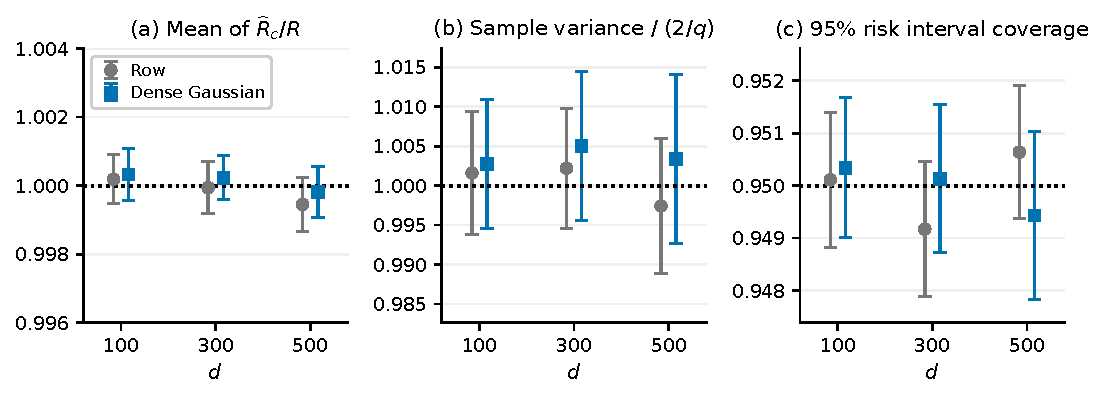
\includegraphics[width=\linewidth]{figures/complementary_calibration.pdf}
    \caption{Conditional calibration of $\widehat R_c$ at $n=300$ and
    $m=150$ ($q=n-m$). Panels show the mean of $\widehat R_c/R$, its conditional
    sample variance divided by $2/q$, and coverage of the nominal
    $95\%$ risk interval. Each setting uses 100 fixed fits and 1,000
    complementary draws per fit. Error bars are pointwise $95\%$
    intervals across fits.}
    \label{fig:simulation-conditional}
\end{figure}

\subsection{Risk curves for three sketch families}
\label{sec:cpal-risk-study}

We next compare mean true risk with mean estimated risk for
$n=100,150,\ldots,1000$ and
$(d/n,m/n)\in\{(0.30,0.50),(0.50,0.70),(0.70,0.90),(0.80,1.00)\}$.
Each setting uses 1,000 independent datasets. Sketch families share the
design and errors within a repetition, while the two error laws share the
design and sketch. For each dataset, error law, and sketch realization,
all criteria assess the same fitted predictor. Alongside
$\hR_o,\hR_u,\hR_{\GCV},\widehat R_c$, we include
\begin{align*}
 \widehat R_B=\frac{\norm{\bu}^2}{n-2d+d^2/m}.
\end{align*}
This row-sampling formula is from
\citet[][Section~3.1, Remark~2, equation~(13)]{bellec2025corrected},
and its use for weighted Haar and dense Gaussian sketches is an empirical
comparison.

% Curves plot empirical means $\bar T$ of the true risk or a risk estimate,
% with $95\%$ Monte Carlo bands $\bar T\pm1.96s(T)/\sqrt{1000}$.

Under Gaussian errors (Figure~\ref{fig:simulation-noninterpolating-accuracy}),
$\hR_o$, $\hR_u$, and $\widehat R_c$ track mean true risk more closely
than GCV when $m<n$; GCV's upward discrepancy is largest at high $d/n$
and persists as $n$ grows. At larger $n$, especially for high $d/n$, the
proposed estimates also track mean true risk more closely than
$\widehat R_B$ for weighted Haar and dense Gaussian sketches, while
$\widehat R_B$ remains accurate for row
sampling. When $m=n$, $\widehat R_c$ is undefined. Row sampling then gives
full-data OLS and $\hR_o=\hR_{\GCV}=\widehat R_B$; for the other sketches,
$\widehat R_B=\hR_{\GCV}$, while $\hR_o$ and $\hR_u$ are closer to mean
true risk.

\begin{figure}[!htbp]
    \centering
    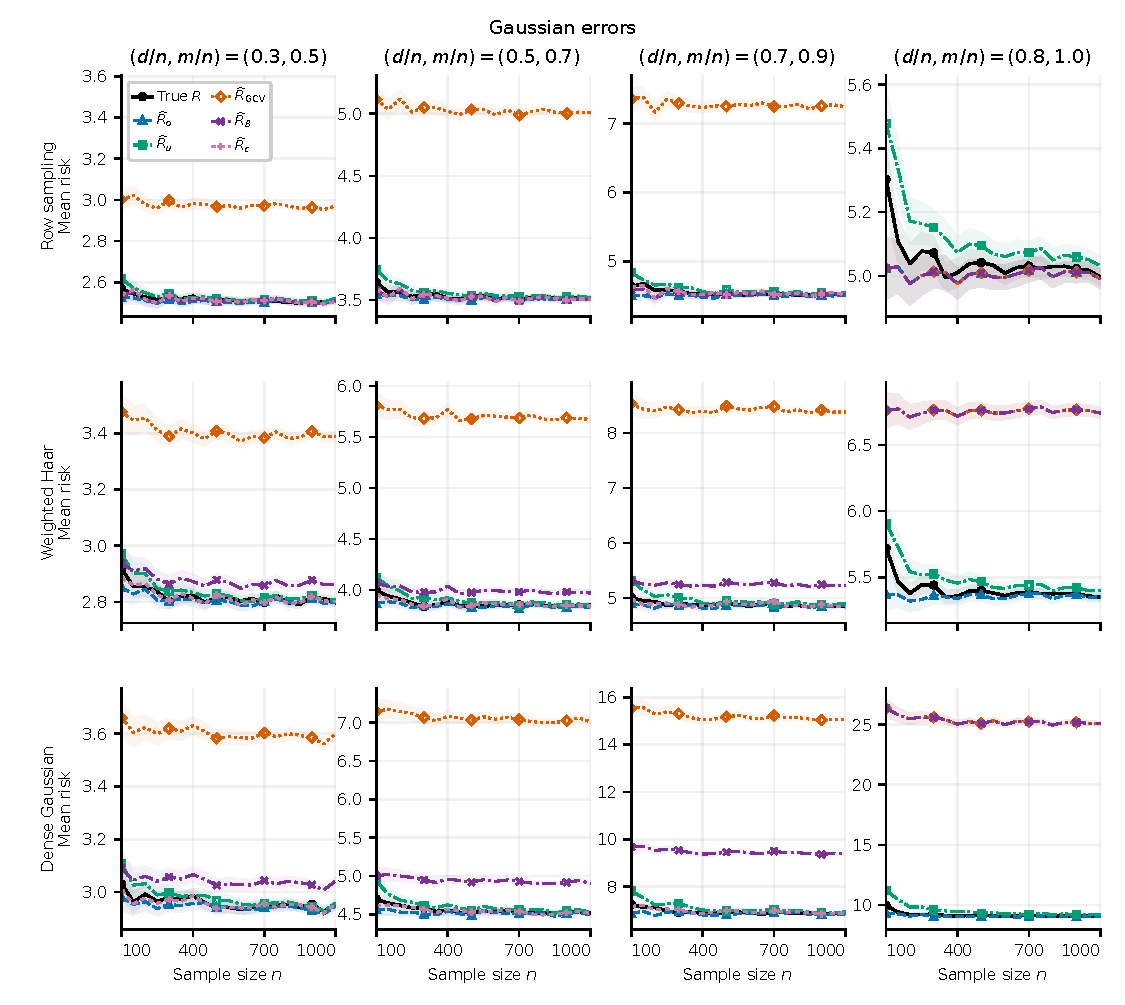
\includegraphics[width=\linewidth]{reports/expanded-risk-20261009/figures/risk_curves_gaussian.pdf}
    \caption{Mean prediction risks and estimates under Gaussian errors.
    Rows give the three sketch families and columns give $(d/n,m/n)$;
    each point uses 1,000 repetitions. The black curve is mean true risk,
    and bands are pointwise $95\%$ Monte Carlo intervals
    $\bar T\pm1.96s(T)/\sqrt{1000}$ for each plotted mean. Bellec's formula is applied
    to every sketch family as an empirical comparison. When $m=n$,
    $\widehat R_c$ is undefined; the observable, GCV, and Bellec curves
    coincide for row sampling, and Bellec's curve coincides with GCV for
    the other sketches. Both axes are linear.}
    \label{fig:simulation-noninterpolating-accuracy}
\end{figure}

\subsection{Comparing estimation MSE}
\label{sec:cpal-mse-study}

The final experiment tests the MSE crossover in
Theorem~\ref{thm:tight-frame-mse-comparison}. With Gaussian errors and row
sampling, we use $n\in\{100,300,500\}$,
$d/n\in\{0.30,0.50,0.70\}$, and five sketch sizes
$m=\operatorname{round}\{n[\rho_*(d/n)+\delta]\}$ for
$\delta\in\{-0.08,-0.04,0,0.04,0.08\}$, with half-ties rounded upward.
All settings satisfy $d+3<m<n$. Each of 1,000 repetitions uses one dataset
and one row permutation for all five sketch sizes, taking the first $m$
indices, scaling rows by $\sqrt{n/m}$, and refitting at each $m$. Define
$a_b=(\hR_o^{(b)}-R^{(b)})^2$ and
$c_b=(\widehat R_c^{(b)}-R^{(b)})^2$. The empirical MSE ratio is
$\widehat\theta=\bar a/\bar c$. With
$v_b=a_b/\bar a-c_b/\bar c$, its paired delta-method interval is
$\widehat\theta\exp\{\pm z_{0.975}s(v)/\sqrt{1000}\}$, where
$z_{0.975}$ is the $0.975$ standard-normal quantile.

Figure~\ref{fig:simulation-mse-threshold} compares empirical and exact MSE
ratios. The crossover $\rho_n^{\#}$
satisfies equality in \eqref{eq:tight-frame-finite-mse-rule} near $\rho_*(d/n)$.
% Exact curves and crossover guides are used for row sampling.
% weighted Haar and dense Gaussian results are empirical comparisons.
Of the 45 intervals, 43 contain the exact ratio. At $\delta=0$ all contain
one; at $\delta=-0.08$ all lie above one, and at $\delta=0.08$ all lie
below one. This confirms lower MSE for $\widehat R_c$ below the crossover
and for $\hR_o$ above it.

\begin{figure}[tb]
    \centering
    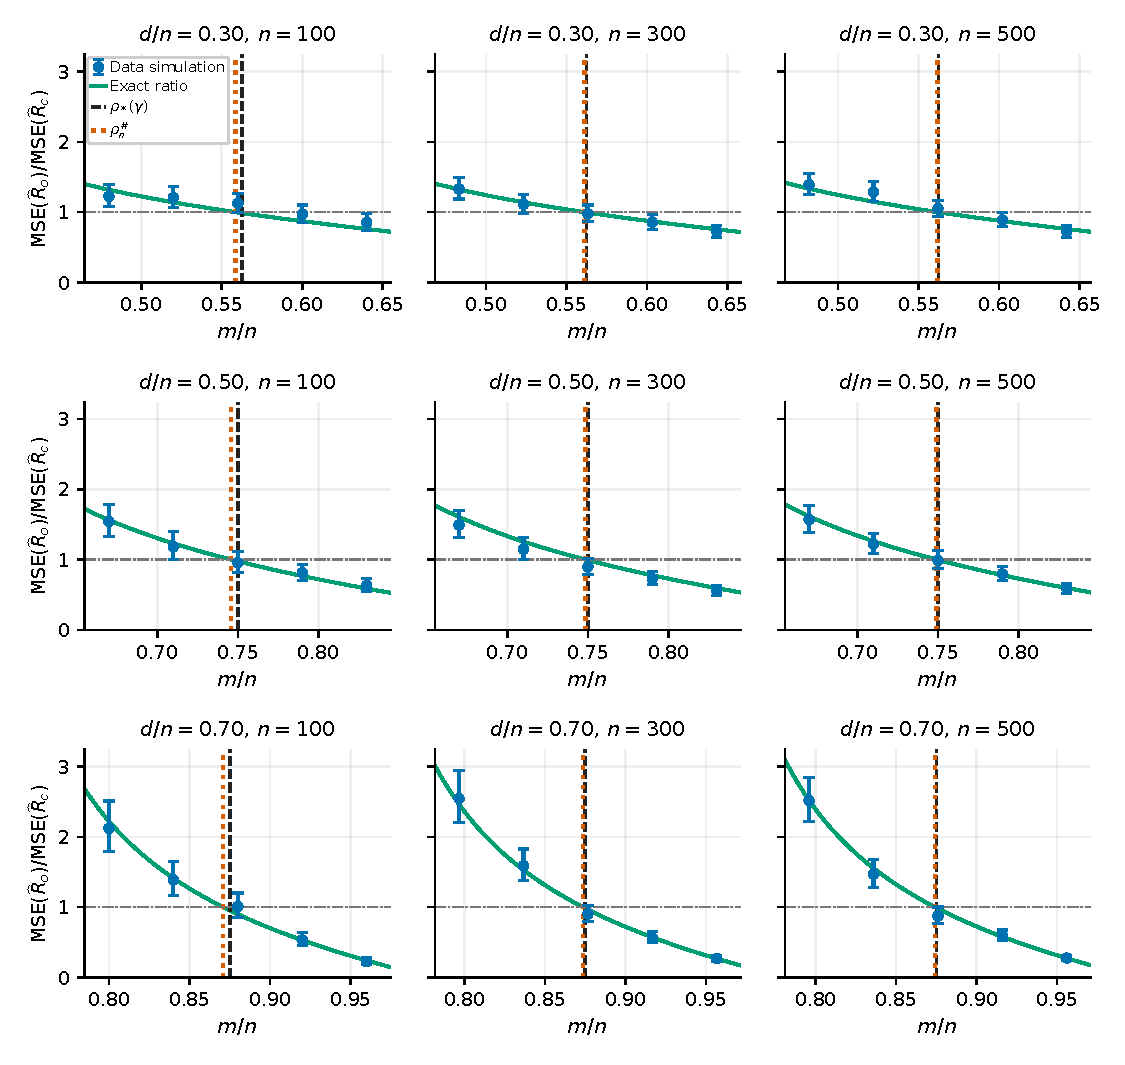
\includegraphics[width=0.95\linewidth]{figures/threshold.pdf}
    \caption{MSE ratio of $\hR_o$ to $\widehat R_c$ under Gaussian data
    and row sampling. Rows give $d/n$, columns give $n$, and the horizontal
    axis gives rounded $m/n$. Points and pointwise $95\%$ paired intervals
    use 1,000 repetitions. The green curve is exact; dashed and dotted lines
    mark $\rho_*(\gamma)$ and $\rho_n^{\#}$. Values above one
    favor $\widehat R_c$.}
    \label{fig:simulation-mse-threshold}
\end{figure}


\section{Discussion}
\label{sec:discussion}

Observation compression supports risk assessment without refitting. The
complementary law holds for Gaussian data and an independent sketch;
row-sampling unbiasedness needs only second moments. The correction bound
permits uniformly sub-Gaussian errors but assumes Gaussian features, $m-d$
proportional to $n$, and a bounded positive spectrum for
$n\bA/\trace(\bA)$. Extensions to non-Gaussian features and less regular
spectra remain open. As $m$ grows, fewer complementary directions remain,
and $\widehat R_c$ is unavailable at $m=n$. Under Gaussian data, the MSE crossover for scaled orthogonal sketches
identifies when $\hR_o$ is more accurate.
The weighted Haar and dense Gaussian MSE comparisons remain empirical;
broader geometries and $m$ near $d$ require further theory.

Assessment needs the original observations or residual summaries, adding
data and computational costs. The simulations use one covariance and
signal. Future work should study other designs, structured sketches,
end-to-end costs, compact sufficient summaries, and data-dependent or
risk-selected sketches that account for design dependence and reused risk.


\FloatBarrier

\clearpage
\bibliography{ref}
\clearpage
\appendix

\section{Additional simulation results}
\label{app:additional-simulations}

The code for reproducing all simulation results is available at
\url{https://github.com/StatResearch-SLAI/RandomSketch}.

\subsection{Risk assessment across sketch families}
\label{sec:simulation-noninterpolating}
\label{app:simulation-accuracy}
Table~\ref{tab:simulation-noninterpolating} summarizes mean prediction
risks and risk estimates at $n=1000$ for both error laws;
Figure~\ref{fig:simulation-noninterpolating-risk-uniform} shows the
additional curves under uniform errors. These summaries describe
calibration across repetitions. To assess estimation accuracy, we compare
each estimate with the true risk of the same fitted predictor. For an
applicable estimate $T$ and
repetition $b=1,\ldots,1000$, the paired errors $\Delta_b=T^{(b)}-R^{(b)}$ give bias $\bar\Delta$ and root mean
squared estimation error (RMSE) $\sqrt{\overline{\Delta^2}}$.
Bias measures average signed error, whereas RMSE also reflects variation
in the errors across fits. Tables~\ref{tab:appendix-accuracy-bias}
and~\ref{tab:appendix-accuracy-rmse} report these quantities at $n=1000$.
Their estimated Monte Carlo standard errors are $s(\Delta)/\sqrt{1000}$ and
$s(\Delta^2)/(2\operatorname{RMSE}\sqrt{1000})$, respectively;
the latter uses the delta method.

The square-sketch setting separates the effects of row space and weighting.
At $n=1000$ and $(d/n,m/n)=(0.80,1.00)$ with Gaussian errors,
the mean true risks are $4.997$, $5.349$, and $9.029$ for row,
weighted Haar, and dense Gaussian sketches. The corresponding means
of $\hR_o$ are $4.991$, $5.352$, and $9.012$, compared with
$4.991$, $6.740$, and $25.079$ for GCV. For the dense Gaussian
sketch, the mean unobservable estimate $\hR_u$ is $9.165$. All three
sketches retain the full observation space, but weighting changes
both the fit and its residual calibration. In the same dense square
setting under uniform errors, mean risk is
$3.021$, the mean $\hR_o$ is $3.002$, and the mean $\hR_u$ is
$3.052$. GCV and Bellec's formula both give a mean of $8.345$,
so the row-sampling expression inherits GCV's mean discrepancy here.
Uniform errors have variance $1/3$, compared with variance one for
Gaussian errors, so the comparison between Gaussian- and uniform-error settings
also changes the noise scale.
The uniform-error curves assess calibration empirically.

Across the 24 settings at $n=1000$, paired mean bias ranges from
$-0.027$ to $0.009$ for $\hR_o$ and from $-0.006$ to $0.136$
for $\hR_u$ (Table~\ref{tab:appendix-accuracy-bias}).
% The complete sample-size results and draw-level records are documented
% in \texttt{Code\_EJS/README.md}.

\begin{figure}[p]
    \centering
    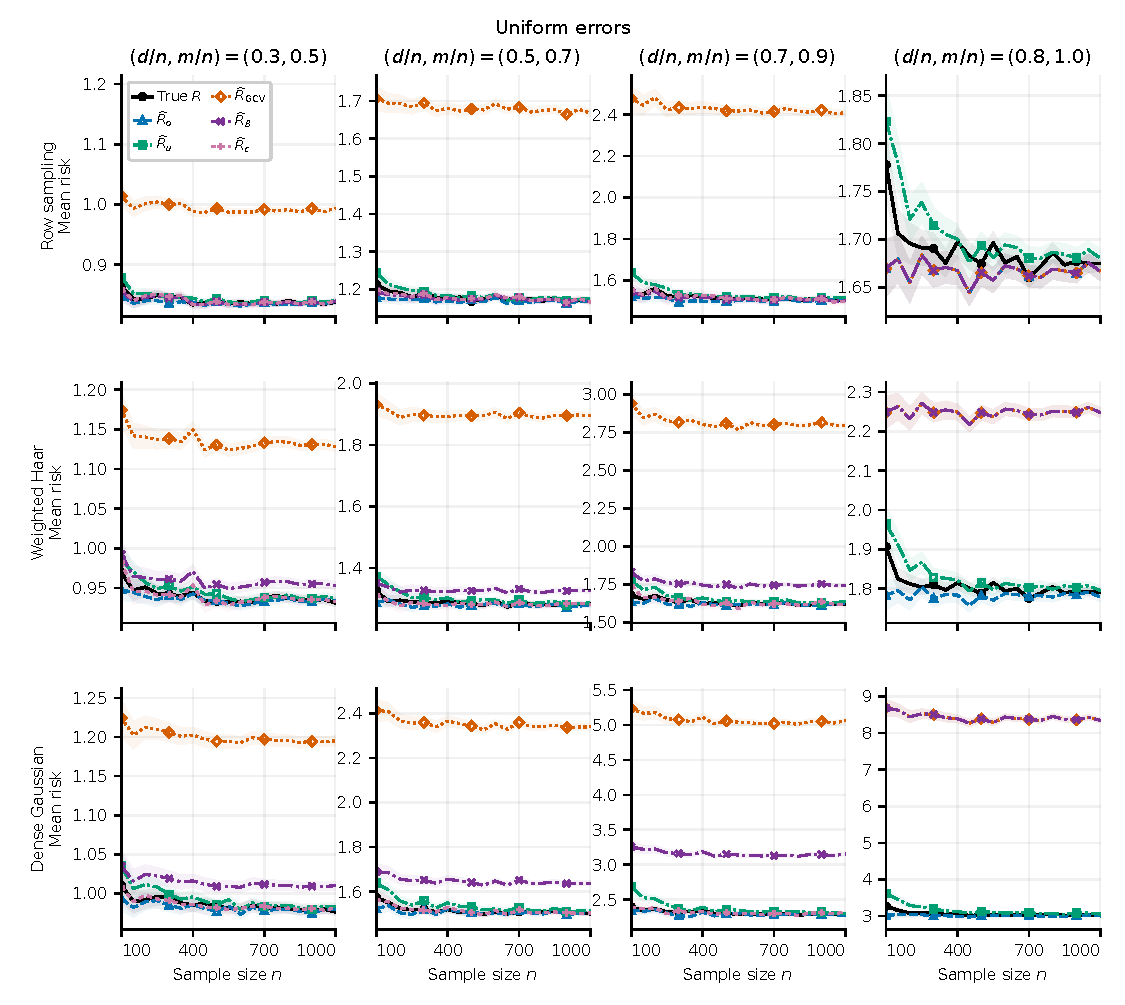
\includegraphics[width=\linewidth]{reports/expanded-risk-20261009/figures/risk_curves_uniform.pdf}
    \caption{Mean prediction risks and risk estimates under independent
    uniform errors on $[-1,1]$, with variance $1/3$. Layout, sample
    sizes, pairing, and Monte Carlo intervals match
    Figure~\ref{fig:simulation-noninterpolating-accuracy}.
    Because the errors are uniform, the complementary-risk curves provide
    empirical calibration rather than an application of the Gaussian
    chi-square law.
    The $\widehat R_B$ curve uses Bellec's formula for all three sketch
    families. The complementary estimate is undefined when $m=n$.}
    \label{fig:simulation-noninterpolating-risk-uniform}
\end{figure}

\begin{table}[p]
    \centering
    \fontsize{7.5}{9.5}\selectfont
    \setlength{\tabcolsep}{2pt}
    \caption{Mean prediction risks and risk estimates at $n=1000$,
    based on 1,000 independent repetitions per setting. Parentheses
    contain Monte Carlo standard errors. The Bellec column uses the same
    formula, denoted $\widehat R_B$, for all three sketch families.
    WH and DG denote weighted Haar and dense Gaussian sketches;
    G and U denote Gaussian and uniform errors.
    A dash denotes the undefined complementary estimate when $m=n$.}
    \label{tab:simulation-noninterpolating}
    \begin{tabular}{@{}lllrrrrrr@{}}
\toprule
Sketch & Errors & $(d/n,m/n)$ & $R$ & $\widehat R_o$ & $\widehat R_u$ & $\widehat R_{\rm GCV}$ & $\widehat R_B$ & $\widehat R_c$ \\
\midrule
Row & G & $(0.3,0.5)$ & 2.507 (0.006) & 2.516 (0.006) & 2.523 (0.006) & 2.972 (0.008) & 2.510 (0.007) & 2.509 (0.008) \\
Row & U & $(0.3,0.5)$ & 0.838 (0.002) & 0.838 (0.002) & 0.841 (0.002) & 0.994 (0.003) & 0.840 (0.002) & 0.841 (0.003) \\
WH & G & $(0.3,0.5)$ & 2.798 (0.008) & 2.798 (0.007) & 2.807 (0.007) & 3.388 (0.010) & 2.862 (0.008) & 2.802 (0.010) \\
WH & U & $(0.3,0.5)$ & 0.931 (0.002) & 0.934 (0.002) & 0.937 (0.002) & 1.128 (0.003) & 0.953 (0.003) & 0.933 (0.003) \\
DG & G & $(0.3,0.5)$ & 2.951 (0.008) & 2.948 (0.008) & 2.959 (0.008) & 3.601 (0.011) & 3.042 (0.009) & 2.956 (0.010) \\
DG & U & $(0.3,0.5)$ & 0.976 (0.003) & 0.979 (0.002) & 0.983 (0.002) & 1.195 (0.003) & 1.010 (0.003) & 0.981 (0.003) \\
\midrule
Row & G & $(0.5,0.7)$ & 3.515 (0.010) & 3.503 (0.009) & 3.520 (0.009) & 5.010 (0.016) & 3.507 (0.011) & 3.508 (0.013) \\
Row & U & $(0.5,0.7)$ & 1.168 (0.003) & 1.171 (0.003) & 1.176 (0.003) & 1.668 (0.005) & 1.168 (0.004) & 1.167 (0.004) \\
WH & G & $(0.5,0.7)$ & 3.855 (0.011) & 3.828 (0.011) & 3.849 (0.011) & 5.671 (0.018) & 3.970 (0.013) & 3.842 (0.015) \\
WH & U & $(0.5,0.7)$ & 1.283 (0.003) & 1.281 (0.004) & 1.288 (0.004) & 1.895 (0.006) & 1.326 (0.004) & 1.282 (0.005) \\
DG & G & $(0.5,0.7)$ & 4.519 (0.014) & 4.495 (0.015) & 4.528 (0.015) & 7.010 (0.023) & 4.907 (0.016) & 4.514 (0.018) \\
DG & U & $(0.5,0.7)$ & 1.501 (0.004) & 1.505 (0.005) & 1.516 (0.005) & 2.339 (0.007) & 1.638 (0.005) & 1.504 (0.006) \\
\midrule
Row & G & $(0.7,0.9)$ & 4.514 (0.013) & 4.512 (0.013) & 4.545 (0.013) & 7.246 (0.027) & 4.515 (0.017) & 4.516 (0.023) \\
Row & U & $(0.7,0.9)$ & 1.504 (0.004) & 1.506 (0.004) & 1.517 (0.004) & 2.409 (0.009) & 1.501 (0.006) & 1.499 (0.008) \\
WH & G & $(0.7,0.9)$ & 4.863 (0.014) & 4.867 (0.015) & 4.907 (0.016) & 8.381 (0.032) & 5.222 (0.020) & 4.838 (0.027) \\
WH & U & $(0.7,0.9)$ & 1.617 (0.005) & 1.624 (0.005) & 1.637 (0.005) & 2.795 (0.010) & 1.741 (0.006) & 1.614 (0.008) \\
DG & G & $(0.7,0.9)$ & 6.863 (0.023) & 6.849 (0.029) & 6.929 (0.030) & 15.063 (0.056) & 9.385 (0.035) & 6.892 (0.038) \\
DG & U & $(0.7,0.9)$ & 2.295 (0.007) & 2.280 (0.010) & 2.306 (0.010) & 5.061 (0.019) & 3.153 (0.012) & 2.325 (0.013) \\
\midrule
Row & G & $(0.8,1.0)$ & 4.997 (0.014) & 4.991 (0.016) & 5.032 (0.016) & 4.991 (0.016) & 4.991 (0.016) & -- \\
Row & U & $(0.8,1.0)$ & 1.675 (0.004) & 1.667 (0.005) & 1.680 (0.005) & 1.667 (0.005) & 1.667 (0.005) & -- \\
WH & G & $(0.8,1.0)$ & 5.349 (0.015) & 5.352 (0.020) & 5.401 (0.020) & 6.740 (0.022) & 6.740 (0.022) & -- \\
WH & U & $(0.8,1.0)$ & 1.793 (0.005) & 1.779 (0.006) & 1.796 (0.006) & 2.248 (0.007) & 2.248 (0.007) & -- \\
DG & G & $(0.8,1.0)$ & 9.029 (0.034) & 9.012 (0.048) & 9.165 (0.050) & 25.079 (0.106) & 25.079 (0.106) & -- \\
DG & U & $(0.8,1.0)$ & 3.021 (0.011) & 3.002 (0.015) & 3.052 (0.015) & 8.345 (0.035) & 8.345 (0.035) & -- \\
\bottomrule
\end{tabular}
% Metric: mean (Monte Carlo SE), n=1000.
% Row/WH/DG: row sampling/weighted Haar/dense Gaussian; G/U: Gaussian/Uniform[-1,1].
% R_B uses Bellec's formula for all sketch families; --: m=n, no complementary directions.

\end{table}

\begin{table}[!htbp]
    \centering
    \footnotesize
    \setlength{\tabcolsep}{2.5pt}
    \caption{Paired empirical bias at $n=1000$ in the expanded
    risk-curve study, with 1,000 repetitions per setting. Parentheses
    contain Monte Carlo standard errors of the empirical mean biases. Dashes have the same meaning as in
    Table~\ref{tab:simulation-noninterpolating}, as do WH, DG, G, and U.}
    \label{tab:appendix-accuracy-bias}
    \begin{tabular}{@{}lllrrrrr@{}}
\toprule
Sketch & Errors & $(d/n,m/n)$ & $\widehat R_o$ & $\widehat R_u$ & $\widehat R_{\rm GCV}$ & $\widehat R_B$ & $\widehat R_c$ \\
\midrule
Row & G & $(0.3,0.5)$ & 0.009 (0.006) & 0.017 (0.006) & 0.465 (0.005) & 0.004 (0.004) & 0.002 (0.005) \\
Row & U & $(0.3,0.5)$ & -0.000 (0.002) & 0.003 (0.002) & 0.156 (0.002) & 0.002 (0.001) & 0.003 (0.002) \\
WH & G & $(0.3,0.5)$ & 0.000 (0.007) & 0.009 (0.007) & 0.590 (0.006) & 0.064 (0.005) & 0.004 (0.006) \\
WH & U & $(0.3,0.5)$ & 0.003 (0.002) & 0.006 (0.002) & 0.197 (0.002) & 0.022 (0.002) & 0.002 (0.002) \\
DG & G & $(0.3,0.5)$ & -0.004 (0.007) & 0.007 (0.007) & 0.650 (0.007) & 0.091 (0.006) & 0.004 (0.006) \\
DG & U & $(0.3,0.5)$ & 0.003 (0.002) & 0.006 (0.002) & 0.219 (0.002) & 0.033 (0.002) & 0.005 (0.002) \\
\midrule
Row & G & $(0.5,0.7)$ & -0.012 (0.011) & 0.005 (0.011) & 1.495 (0.011) & -0.008 (0.008) & -0.007 (0.009) \\
Row & U & $(0.5,0.7)$ & 0.002 (0.003) & 0.008 (0.003) & 0.500 (0.004) & -0.001 (0.003) & -0.001 (0.003) \\
WH & G & $(0.5,0.7)$ & -0.027 (0.012) & -0.006 (0.012) & 1.816 (0.013) & 0.114 (0.009) & -0.013 (0.010) \\
WH & U & $(0.5,0.7)$ & -0.002 (0.004) & 0.005 (0.004) & 0.611 (0.004) & 0.043 (0.003) & -0.001 (0.003) \\
DG & G & $(0.5,0.7)$ & -0.024 (0.015) & 0.009 (0.015) & 2.491 (0.016) & 0.388 (0.011) & -0.005 (0.012) \\
DG & U & $(0.5,0.7)$ & 0.004 (0.005) & 0.015 (0.005) & 0.839 (0.005) & 0.137 (0.004) & 0.003 (0.004) \\
\midrule
Row & G & $(0.7,0.9)$ & -0.002 (0.017) & 0.031 (0.017) & 2.732 (0.024) & 0.001 (0.015) & 0.002 (0.020) \\
Row & U & $(0.7,0.9)$ & 0.002 (0.006) & 0.013 (0.006) & 0.905 (0.008) & -0.003 (0.005) & -0.005 (0.007) \\
WH & G & $(0.7,0.9)$ & 0.004 (0.019) & 0.043 (0.019) & 3.517 (0.026) & 0.358 (0.017) & -0.025 (0.022) \\
WH & U & $(0.7,0.9)$ & 0.007 (0.007) & 0.020 (0.007) & 1.177 (0.008) & 0.124 (0.005) & -0.003 (0.007) \\
DG & G & $(0.7,0.9)$ & -0.013 (0.031) & 0.067 (0.031) & 8.200 (0.044) & 2.523 (0.026) & 0.029 (0.030) \\
DG & U & $(0.7,0.9)$ & -0.015 (0.011) & 0.011 (0.011) & 2.766 (0.015) & 0.858 (0.009) & 0.030 (0.010) \\
\midrule
Row & G & $(0.8,1.0)$ & -0.005 (0.022) & 0.036 (0.022) & -0.005 (0.022) & -0.005 (0.022) & -- \\
Row & U & $(0.8,1.0)$ & -0.008 (0.007) & 0.005 (0.007) & -0.008 (0.007) & -0.008 (0.007) & -- \\
WH & G & $(0.8,1.0)$ & 0.003 (0.025) & 0.052 (0.025) & 1.391 (0.026) & 1.391 (0.026) & -- \\
WH & U & $(0.8,1.0)$ & -0.013 (0.008) & 0.003 (0.008) & 0.455 (0.009) & 0.455 (0.009) & -- \\
DG & G & $(0.8,1.0)$ & -0.018 (0.051) & 0.136 (0.053) & 16.049 (0.092) & 16.049 (0.092) & -- \\
DG & U & $(0.8,1.0)$ & -0.019 (0.016) & 0.031 (0.017) & 5.324 (0.031) & 5.324 (0.031) & -- \\
\bottomrule
\end{tabular}
% Metric: paired_bias (Monte Carlo SE), n=1000.
% Row/WH/DG: row sampling/weighted Haar/dense Gaussian; G/U: Gaussian/Uniform[-1,1].
% R_B uses Bellec's formula for all sketch families; --: m=n, no complementary directions.

\end{table}

\begin{table}[tb]
    \centering
    \footnotesize
    \setlength{\tabcolsep}{2.5pt}
    \caption{Empirical RMSE at $n=1000$ in the expanded risk-curve
    study, with 1,000 repetitions per setting. Parentheses contain
    delta-method Monte Carlo standard errors. Dashes have the same
    meaning as in Table~\ref{tab:simulation-noninterpolating}, as do
    WH, DG, G, and U.}
    \label{tab:appendix-accuracy-rmse}
    \begin{tabular}{@{}lllrrrrr@{}}
\toprule
Sketch & Errors & $(d/n,m/n)$ & $\widehat R_o$ & $\widehat R_u$ & $\widehat R_{\rm GCV}$ & $\widehat R_B$ & $\widehat R_c$ \\
\midrule
Row & G & $(0.3,0.5)$ & 0.174 (0.004) & 0.175 (0.004) & 0.493 (0.005) & 0.142 (0.003) & 0.156 (0.003) \\
Row & U & $(0.3,0.5)$ & 0.060 (0.001) & 0.060 (0.001) & 0.165 (0.002) & 0.046 (0.001) & 0.051 (0.001) \\
WH & G & $(0.3,0.5)$ & 0.213 (0.005) & 0.214 (0.005) & 0.622 (0.006) & 0.181 (0.005) & 0.185 (0.005) \\
WH & U & $(0.3,0.5)$ & 0.068 (0.002) & 0.069 (0.002) & 0.206 (0.002) & 0.057 (0.001) & 0.059 (0.001) \\
DG & G & $(0.3,0.5)$ & 0.216 (0.005) & 0.218 (0.005) & 0.683 (0.007) & 0.200 (0.005) & 0.197 (0.005) \\
DG & U & $(0.3,0.5)$ & 0.069 (0.002) & 0.070 (0.002) & 0.228 (0.002) & 0.065 (0.001) & 0.061 (0.001) \\
\midrule
Row & G & $(0.5,0.7)$ & 0.340 (0.008) & 0.340 (0.008) & 1.535 (0.011) & 0.247 (0.006) & 0.282 (0.006) \\
Row & U & $(0.5,0.7)$ & 0.110 (0.003) & 0.110 (0.003) & 0.513 (0.004) & 0.079 (0.002) & 0.091 (0.002) \\
WH & G & $(0.5,0.7)$ & 0.377 (0.009) & 0.377 (0.009) & 1.859 (0.013) & 0.301 (0.006) & 0.311 (0.007) \\
WH & U & $(0.5,0.7)$ & 0.125 (0.003) & 0.125 (0.003) & 0.625 (0.004) & 0.101 (0.002) & 0.103 (0.002) \\
DG & G & $(0.5,0.7)$ & 0.487 (0.012) & 0.488 (0.012) & 2.539 (0.016) & 0.519 (0.010) & 0.386 (0.009) \\
DG & U & $(0.5,0.7)$ & 0.157 (0.004) & 0.159 (0.004) & 0.854 (0.005) & 0.177 (0.003) & 0.127 (0.003) \\
\midrule
Row & G & $(0.7,0.9)$ & 0.524 (0.012) & 0.529 (0.012) & 2.831 (0.024) & 0.487 (0.011) & 0.641 (0.014) \\
Row & U & $(0.7,0.9)$ & 0.184 (0.004) & 0.185 (0.004) & 0.941 (0.008) & 0.164 (0.004) & 0.216 (0.005) \\
WH & G & $(0.7,0.9)$ & 0.594 (0.014) & 0.598 (0.014) & 3.615 (0.027) & 0.637 (0.014) & 0.699 (0.016) \\
WH & U & $(0.7,0.9)$ & 0.209 (0.005) & 0.211 (0.005) & 1.207 (0.008) & 0.210 (0.005) & 0.218 (0.005) \\
DG & G & $(0.7,0.9)$ & 0.979 (0.023) & 0.991 (0.023) & 8.319 (0.045) & 2.653 (0.026) & 0.943 (0.022) \\
DG & U & $(0.7,0.9)$ & 0.335 (0.008) & 0.339 (0.008) & 2.806 (0.015) & 0.904 (0.009) & 0.327 (0.007) \\
\midrule
Row & G & $(0.8,1.0)$ & 0.681 (0.015) & 0.686 (0.015) & 0.681 (0.015) & 0.681 (0.015) & -- \\
Row & U & $(0.8,1.0)$ & 0.227 (0.005) & 0.228 (0.005) & 0.227 (0.005) & 0.227 (0.005) & -- \\
WH & G & $(0.8,1.0)$ & 0.777 (0.018) & 0.784 (0.018) & 1.623 (0.025) & 1.623 (0.025) & -- \\
WH & U & $(0.8,1.0)$ & 0.251 (0.006) & 0.252 (0.006) & 0.531 (0.008) & 0.531 (0.008) & -- \\
DG & G & $(0.8,1.0)$ & 1.622 (0.038) & 1.671 (0.041) & 16.311 (0.093) & 16.311 (0.093) & -- \\
DG & U & $(0.8,1.0)$ & 0.516 (0.012) & 0.526 (0.013) & 5.413 (0.031) & 5.413 (0.031) & -- \\
\bottomrule
\end{tabular}
% Metric: rmse (Monte Carlo SE), n=1000.
% Row/WH/DG: row sampling/weighted Haar/dense Gaussian; G/U: Gaussian/Uniform[-1,1].
% R_B uses Bellec's formula for all sketch families; --: m=n, no complementary directions.

\end{table}

\FloatBarrier

\subsection{Additional MSE comparisons}
\label{sec:simulation-complementary-corrected}
\label{sec:simulation-mse-threshold}
\label{app:simulation-mse-sketch-families}
Figures~\ref{fig:simulation-mse-weighted-haar} and
\ref{fig:simulation-mse-dense-gaussian} extend the MSE comparison to
weighted Haar and dense Gaussian sketches. We use the datasets,
sketch-size grid, repetitions and paired MSE intervals of
Section~\ref{sec:cpal-mse-study}, with $\rho_*(d/n)$ as a common grid
reference for these empirical comparisons.

For weighted Haar sketches, generate the orthonormal Haar rows at the
largest tested size and take the first $m$ rows for each $m$.
Apply alternating weights one and two, and normalize separately at each
$m$ so that $\trace(\bS^\top\bS)=n$.
For dense Gaussian sketches, generate one standard Gaussian matrix
with as many rows as the largest tested size, take its first $m$ rows,
and divide by $\sqrt m$. Each family uses its own random construction,
and the compressed model is refitted at every $m$.

For both families, all eighteen intervals with $\delta<0$ lie above one.
At the nominal central settings, $\delta=0$, the weighted Haar ratios
range from $0.952$ to $1.166$; seven intervals contain one and two lie
above it. The dense Gaussian ratios range from $1.021$ to $1.386$;
seven intervals lie above one and two contain it. All nine dense Gaussian
central point estimates exceed one.
At $\delta=0.04$, six weighted Haar intervals and four dense Gaussian
intervals lie below one; the remaining intervals contain one.
At $\delta=0.08$, all nine weighted Haar intervals and eight dense
Gaussian intervals lie below one; the remaining dense Gaussian interval
contains one. The empirical ratios decrease across the five tested
sketch sizes in every panel. For comparison, under row sampling,
seventeen of the eighteen intervals with $\delta<0$
lie above one and seventeen of the eighteen with $\delta>0$ lie below
one; the remaining interval on each side contains one.
The central ratios at $\delta=0$ range from $0.875$ to $1.125$.
Across the row-sampling dimension settings, the exact crossover lies below
$\rho_*(d/n)$ by less than $1/n$.

\begin{figure}[htbp]
    \centering
    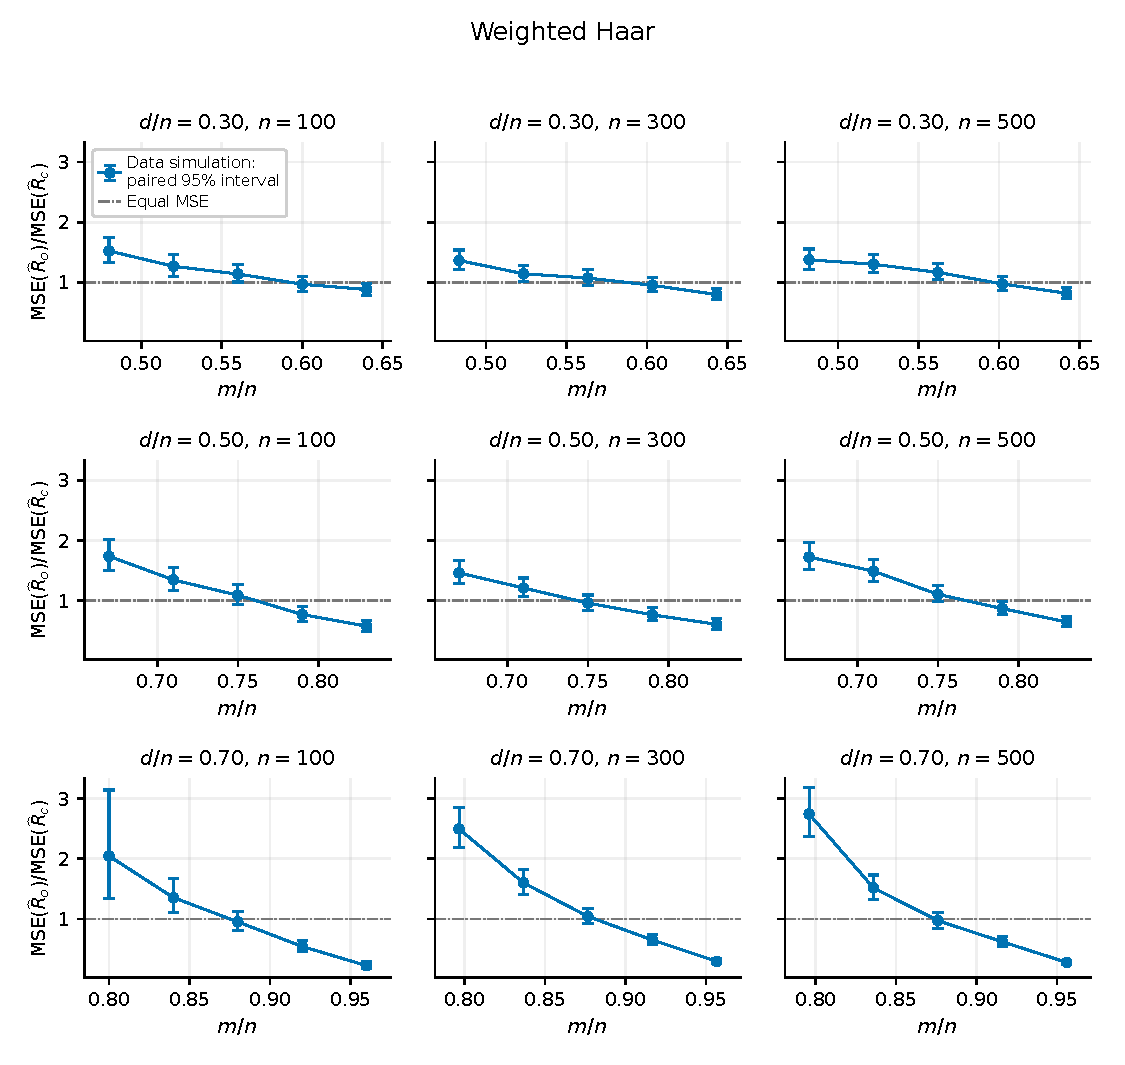
\includegraphics[width=\linewidth]{figures/threshold_weighted_haar.pdf}
    \caption{Empirical MSE ratio of the corrected to the complementary
    risk estimator for weighted Haar sketches under Gaussian data.
    Rows give $d/n\in\{0.30,0.50,0.70\}$ and columns give
    $n\in\{100,300,500\}$; the horizontal axis is the actual $m/n$.
    Points and error bars show ratios and pointwise $95\%$ paired
    Monte Carlo intervals based on 1,000 repetitions per setting.
    Ratios above one favor the complementary estimate; ratios below
    one favor the corrected estimate. The horizontal line marks equal
    MSE, and connecting segments only guide the eye. Only empirical
    ratios are shown because the scaled orthogonal formula does not apply to
    the alternating weights.}
    \label{fig:simulation-mse-weighted-haar}
\end{figure}

\begin{figure}[p]
    \centering
    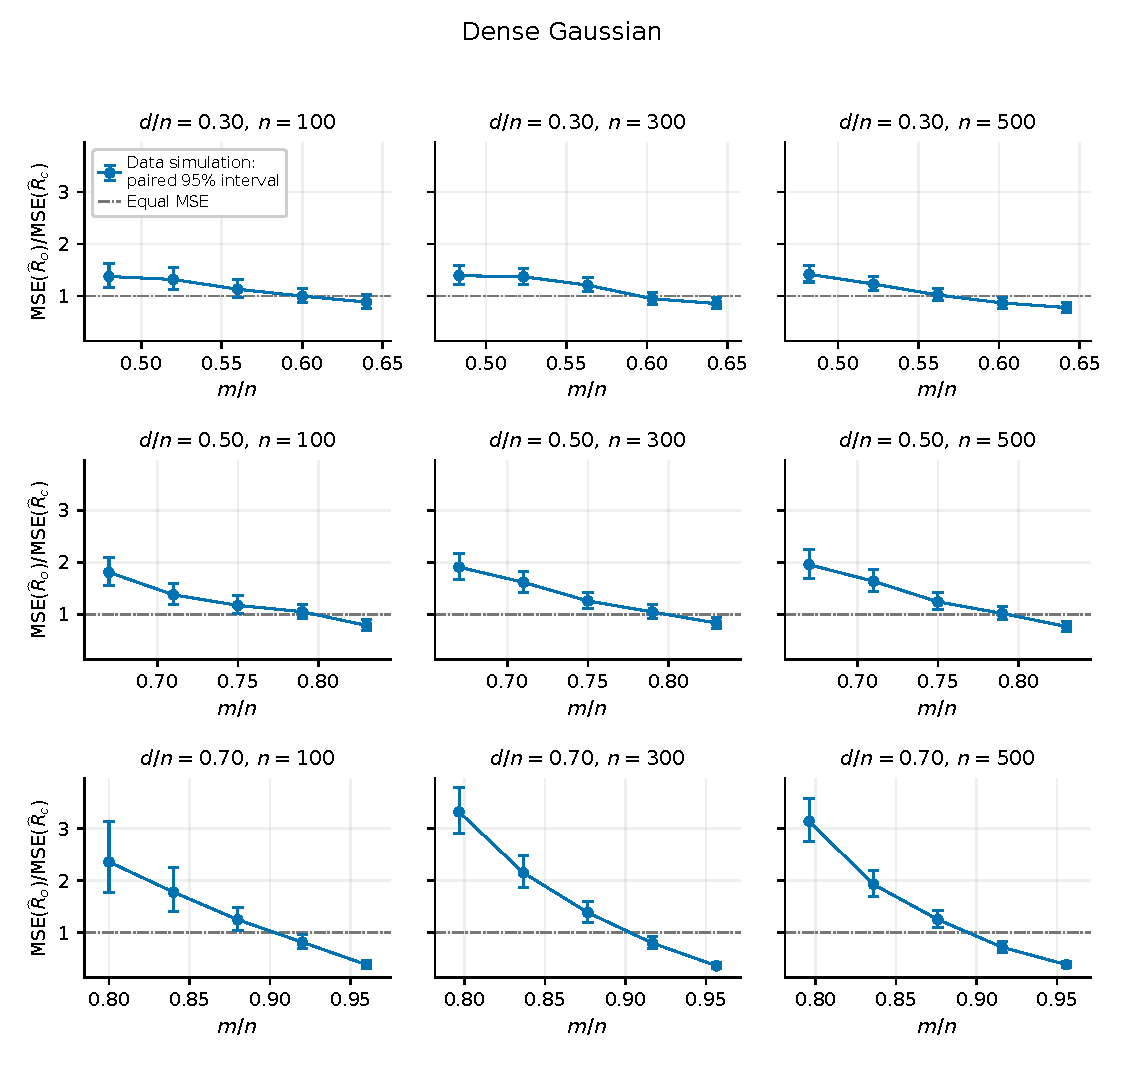
\includegraphics[width=\linewidth]{figures/threshold_dense_gaussian.pdf}
    \caption{Empirical MSE ratio of the corrected to the complementary
    risk estimator for raw dense Gaussian sketches under Gaussian data.
    Layout, dimensions, pairing, repetitions, and intervals match
    Figure~\ref{fig:simulation-mse-weighted-haar}.
    Ratios above one favor the complementary estimate; ratios below
    one favor the corrected estimate. The horizontal line marks equal
    MSE, and connecting segments only guide the eye. Only empirical
    ratios are shown because a dense Gaussian sketch is not a scaled orthogonal sketch.}
    \label{fig:simulation-mse-dense-gaussian}
\end{figure}

\FloatBarrier

\clearpage
% Relocated from the approved pre-revision source; mathematical bodies and original labels are retained.
\section{Notation and supporting results}
\label{app:extended-results}

This appendix supplies the notation and auxiliary results used in the
proofs. After a compact setup, we develop the moment and trace bounds
needed for the corrected estimator. Appendices~\ref{app:overparameterized-proofs}
and~\ref{app:underparameterized-proofs} give the proofs in the order of
the main text.
For matrices, $\preceq$ denotes the positive-semidefinite order,
$\|\cdot\|_{\mathrm{op}}$ the operator norm, and
$\|\cdot\|_{\mathrm F}$ the Frobenius norm.
The table below locates each main proof.
\begin{center}
\begin{tabular}{@{}ll@{}}
\toprule
Main result & Proof sections \\
\midrule
Theorem~\ref{thm:cpal-complementary-law} & \ref{app:proof-complementary-validation} \\
Theorem~\ref{thm:cpal-corrected-accuracy} & \ref{app:proof-R-sens-general} and \ref{app:proof-R-obs-general} \\
Theorem~\ref{thm:cpal-risk-benchmarks} & \ref{app:proof-tight-frame-risk} and \ref{app:dense-Gaussian-proof} \\
Theorem~\ref{thm:tight-frame-mse-comparison} & \ref{app:proof-tight-frame-mse-comparison} \\
Theorem~\ref{thm:cpal-mse-comparison} & \ref{app:proof-tight-frame-asymptotic-mse-threshold} \\
\bottomrule
\end{tabular}
\end{center}

\subsection{Proof setup and assumptions}
\label{app:proof-setup}

\begin{assumption}
\label{assu:model-sketch}
The observations, covariance bounds, errors, sketch and independent test
pair satisfy the model conditions of Section~\ref{sec:meth}. Write
$0<c_{\bSigma}\leq C_{\bSigma}<\infty$ for the fixed constants,
independent of $n$, satisfying
$c_{\bSigma}\bI_d\preceq\bSigma\preceq C_{\bSigma}\bI_d$.
\end{assumption}\vsReadingSymbol{$c_{\bSigma}$}{$c_{\bSigma}$ is a fixed positive constant, independent of $n$, satisfying $c_{\bSigma}\bI_d\preceq\bSigma$ and $c_{\bSigma}\leq C_{\bSigma}$.}\vsReadingSymbol{$C_{\bSigma}$}{$C_{\bSigma}$ is a fixed finite positive constant, independent of $n$, satisfying $\bSigma\preceq C_{\bSigma}\bI_d$.}
We use the fit and residual notation of
Section~\ref{sec:underparameterized-transfer}, and write
\begin{align*}
    \bB&:=\bS\bX,
    &\bM&=\bB^\top\bB,
    &\bh&:=\hbbeta_{\bS}-\bbeta^*.
\end{align*}
\begin{assumption}
\label{assu:noninterpolating}
In addition to Assumption~\ref{assu:model-sketch}, suppose
$1\leq d<m\leq n$ and $\rank(\bS\bX)=d$ almost surely.
\end{assumption}
Let $\bP_{\bB}:=\bB(\bB^\top\bB)^{-1}\bB^\top$.
The residual sketch mass satisfies
\begin{align*}
    b_{\bA}
    =\trace\!\left\{(\bI_m-\bP_{\bB})\bS\bS^\top\right\}>0,
\end{align*}
because $\bS\bS^\top\succ0$ and $\bI_m-\bP_{\bB}$ is a projector
of rank $m-d>0$. If
$\lambda_1(\bA)\geq\cdots\geq\lambda_m(\bA)>0$ are the positive
eigenvalues of $\bA$, Ky Fan's inequality gives
\begin{align}
    b_{\bA}\geq\sum_{j=d+1}^{m}\lambda_j(\bA).
    \label{eq:bA-spectral-lower}
\end{align}

\vsReadingSymbol{$\bB$}{$\bB\in\R^{m\times d}$ denotes $\bS\bX$ except where explicitly rebound locally. In Lemma~\ref{lem:M-inverse-bound}: In the proof's bound for the sketched least-squares map, $\bB=\bLambda^{1/2}\bG_0$ locally, where $\bG_0\in\R^{m\times d}$ is the Gaussian matrix used in that proof.}

\vsReadingSymbol{$\bh$}{$\bh=\hbbeta_{\bS}-\bbeta^*$ is the coefficient error computed from the response used in the expectation under consideration. In Lemma~\ref{lem:balanced-trace-Stein-bounds}, Proposition~\ref{prop:trace-calibration-general}: Under $\E_{\rm aux}$, recompute $\bh$ using the auxiliary response and $\bbeta^*=\boldzero$; under the original response law use the original coefficient error.}

The fit and both corrected estimators are invariant to the overall
sketch scale. Replacing $\bS$ by $\sqrt c\,\bS$ for any $c>0$ multiplies
$\bA$, $b_{\bA}$, and $\br$ by $c$ and $t_{\bSigma}$ by $c^{-1}$,
leaving the corrected residuals unchanged. The discrepancy
$t_{\bSigma}-d/b_{\bA}$ scales by $c^{-1}$. We therefore use
\begin{align*}
    \overline{\bS}
    &:=\left\{\frac{n}{\trace(\bA)}\right\}^{1/2}\bS,
    &\overline{\bA}&:=\overline{\bS}^{\top}\overline{\bS}.
\end{align*}
In the balanced-sketch calculations from
Section~\ref{app:balanced-transfer-setup} through
Section~\ref{app:proof-trace-calibration-general}, we reuse
$(\bS,\bA,b_{\bA},\br,t_{\bSigma})$ for the normalized quantities,
so $\trace(\bA)=n$ almost surely. The sketch-specific calculations in
Appendix~\ref{app:underparameterized-proofs} retain the natural scalings
stated there.

\begin{assumption}
\label{assu:Gaussian-Stein-design}
In addition to Assumption~\ref{assu:noninterpolating}, suppose
$\bX=\bZ\bSigma^{1/2}$, where $\bZ$ has independent standard Gaussian
entries and is independent of $(\bS,\bep)$.
The errors are uniformly sub-Gaussian: there exists a constant
$K_\varepsilon<\infty$, independent of $n$, such that
$\sup_n\norm{\varepsilon_1}_{\psi_2}\leq K_\varepsilon$, where
\begin{align*}
    \norm{W}_{\psi_2}
    :=\inf\left\{t>0:\E\exp(W^2/t^2)\leq2\right\}.
\end{align*}
Use the normalization $\trace(\bA)=n$, and let
$\bA=\bU\bLambda\bU^\top$ be an $\bS$-measurable spectral
decomposition, where $\bU\in\R^{n\times m}$ satisfies
$\bU^\top\bU=\bI_m$ and $\bLambda$ contains the positive eigenvalues
of $\bA$. There exist deterministic constants $n_0\geq1$,
$0<c_-\leq c_+<\infty$, and $\kappa>0$, independent of $n$, such
that, for every $n\geq n_0$, almost surely,
\begin{align}
    c_-\bI_m\preceq\bLambda\preceq c_+\bI_m,
    \qquad
    m-d\geq\kappa n.
    \label{eq:balanced-sketch-conditions}
\end{align}
\end{assumption}\vsReading{In the balanced-sketch calculations, $(\bS,\bA)$ denote the normalized quantities $(\overline{\bS},\overline{\bA})$ defined in Section~\ref{app:proof-setup}, so $\trace(\bA)=n$ almost surely.}\vsReadingSymbol{$K_\varepsilon$}{$K_\varepsilon<\infty$ is a deterministic constant independent of $n$ controlling the error $\psi_2$ norm, using the absolute convention unless the relative convention is explicitly invoked. In Lemma~\ref{lem:opnorm-X-bound}: For the explicitly stated relative version of the noise-energy bound, $K_\varepsilon$ instead satisfies $\norm{\varepsilon_1}_{\psi_2}\leq K_\varepsilon\sigma$; this convention applies to that version only.}\vsReadingSymbol{$\bU$}{$\bU$ is an orthonormal-column matrix, with its column count and defining decomposition specified locally. In Theorem~\ref{thm:cpal-corrected-accuracy}, Lemma~\ref{lem:dot-beta}, Lemma~\ref{lem:dot-r}, Lemma~\ref{lem:dot-rh}, Lemma~\ref{lem:dot-hxh}, Lemma~\ref{lem:dot-rxr}, Lemma~\ref{lem:dot-rxxr}, Lemma~\ref{lem:dot-hxxh}, Lemma~\ref{lem:opnorm-X-bound}, Lemma~\ref{lem:M-inverse-bound}, Lemma~\ref{lem:balanced-Stein-sufficient-conditions}, Lemma~\ref{lem:balanced-moment-bounds}, Proposition~\ref{prop:Stein-risk-from-moments}, Proposition~\ref{eq:Q-identity-Sigma}, Lemma~\ref{lem:balanced-remainder-bounds}, Lemma~\ref{lem:balanced-trace-Stein-bounds}, Lemma~\ref{lem:balanced-exceptional-weight}, Proposition~\ref{prop:trace-calibration-general}: $\bU\in\R^{n\times m}$ is an $\bS$-measurable choice in $\bA=\bU\bLambda\bU^\top$, with $\bU^\top\bU=\bI_m$ and $\bLambda$ containing the positive eigenvalues; it is held fixed in derivatives with respect to $\bZ$. In Theorem~\ref{thm:cpal-risk-benchmarks}: In the dense Gaussian proof, $\bU=\bZ(\bZ^\top\bZ)^{-1/2}\in\R^{n\times d}$ is the thin polar factor of $\bZ$, with $\bU^\top\bU=\bI_d$; $[\bU,\bV]$ is a measurable orthogonal completion.}\vsReadingSymbol{$\bLambda$}{$\bLambda\in\R^{m\times m}$ is the diagonal matrix of positive eigenvalues in an $\bS$-measurable decomposition $\bA=\bU\bLambda\bU^\top$, where $\bU^\top\bU=\bI_m$ and $\trace(\bA)=n$; for all sufficiently large $n$, $c_-\bI_m\preceq\bLambda\preceq c_+\bI_m$ almost surely.}
Together with \eqref{eq:bA-spectral-lower}, these conditions imply
\begin{align*}
    b_{\bA}\geq c_-(m-d)\geq c_-\kappa n,
    \qquad \frac{n}{b_{\bA}}\leq\frac{1}{c_-\kappa}.
\end{align*}

\subsection{Coordinates and differential identities}
\label{app:balanced-transfer-setup}
The correction argument in this and the next three subsections uses the
trace-normalized representative and
Assumption~\ref{assu:Gaussian-Stein-design}. All fixed-order moment bounds
are uniform for sufficiently large $n$. The threshold may depend on the
fixed moment order, and the constants may depend only on the fixed model
and sketch parameters. Unless stated otherwise, derivatives are
pathwise with respect to $\bZ$, with $\bS$, $\bSigma$, $\bbeta^*$, and
the structural noise $\bep=\by-\bX\bbeta^*$ held fixed. Write
\begin{align*}
    b&:=b_{\bA},
    & \bq&:=\bSigma^{1/2}\bh,\\
    \widetilde{\bM}&:=\bZ^\top\bA\bZ,
    & \bL&:=\bA\bZ\widetilde{\bM}^{-1},
    & \bell&:=\bL\bq,\\
    \bv&:=\bZ\bq-t_{\bSigma}\br,
    & G_{\bSigma}&:=\norm{\bq}^2+\frac{1}{n}\norm{\br}^2
      =\norm{\bSigma^{1/2}\bh}^2+\frac{1}{n}\norm{\br}^2.
\end{align*}
In these supporting calculations, the trace coefficient is
\begin{align*}
    t_{\bSigma}=\trace(\bSigma\bM^{-1})
       =\trace(\widetilde{\bM}^{-1}).
\end{align*}
Here $\bq$ measures coefficient error on the prediction scale,
$\bq=\bL^\top\bep$ expresses it in terms of training noise, and
$\br=\bA(\bep-\bZ\bq)$ is the weighted residual. Moments of $\bL$
and $\br$ control the derivatives used below. Also write
$\bG_0:=\bU^\top\bZ\in\R^{m\times d}$, where $\bU$ comes
from the standing spectral decomposition of $\bA$. We use
$[d]:=\{1,\ldots,d\}$ and let $\be_j$ denote a standard basis vector,
with its ambient dimension determined by context.
For any weakly differentiable map
$\bff:\R^{n\times d}\to\R^p$, define its derivative energy by
\begin{equation*}
    \calE_{\bff}:=\sum_{i=1}^n\sum_{j=1}^d
    \norm{\pdv{\bff}{z_{ij}}}^2.
\end{equation*}
The value of $p$ will be clear from the map under consideration.

\vsReadingSymbol{$\bq$}{$\bq$ is an $\R^d$-valued field of the design coordinates. In Theorem~\ref{thm:cpal-corrected-accuracy}, Theorem~\ref{thm:cpal-risk-benchmarks}, Theorem~\ref{thm:tight-frame-mse-comparison}, Lemma~\ref{lem:dot-beta}, Lemma~\ref{lem:dot-r}, Lemma~\ref{lem:dot-rh}, Lemma~\ref{lem:dot-hxh}, Lemma~\ref{lem:dot-rxr}, Lemma~\ref{lem:dot-rxxr}, Lemma~\ref{lem:dot-hxxh}, Lemma~\ref{lem:M-inverse-bound}, Lemma~\ref{lem:balanced-Stein-sufficient-conditions}, Lemma~\ref{lem:balanced-moment-bounds}, Lemma~\ref{lem:influence-from-moments}, Proposition~\ref{prop:Stein-risk-from-moments}, Proposition~\ref{eq:Q-identity-Sigma}, Lemma~\ref{lem:balanced-remainder-bounds}, Lemma~\ref{lem:balanced-trace-Stein-bounds}, Lemma~\ref{lem:balanced-exceptional-weight}, Proposition~\ref{prop:trace-calibration-general}: $\bq=\bSigma^{1/2}(\hbbeta_{\bS}-\bbeta^*)=\widetilde{\bM}^{-1}\bZ^\top\bA\bep=\bL^\top\bep$ is the prediction-scale coefficient error; its design derivatives hold $\bS$, $\bSigma$, $\bbeta^*$ and $\bep$ fixed. In Lemma~\ref{lem:derivative-energy-from-inverse-moments}: $\bq\in\R^d$ is a general random vector field satisfying the displayed derivative identities and moment assumptions; it need not be a least-squares coefficient error. In Lemma~\ref{lem:Stein-remainders-from-moments}: Conditional on $(\bS,\bep)$, $\bq=\bq(\bZ,\bS,\bep)$ is a general $C^\infty$ field in $\bZ$; its meaning is not restricted to the coefficient-error specialization. In Lemma~\ref{lem:balanced-trace-Stein-bounds}, Proposition~\ref{prop:trace-calibration-general}: In expressions under $\E_{\rm aux}$, recompute $\bq$ from the auxiliary response with $\bbeta^*=\boldzero$; expressions under the original response law retain its original coefficient-error field. In another result of the paper: Conditional on $(\bS,\bep)$, $\bq=\bq(\bZ,\bS,\bep)$ is a general $C^\infty$ field in $\bZ$ under the second-order moment premises; it need not be the prediction-scale coefficient error.}

\vsReadingSymbol{$\bL$}{$\bL$ is an $n\times d$ real matrix with the specialization specified in its scoped uses. In Lemma~\ref{lem:derivative-energy-from-inverse-moments}: $\bL$ is a generic random matrix in $\R^{n\times d}$ satisfying $\partial\bq/\partial z_{ij}=\bK\be_jr_i-\bL^\top\be_iq_j$ almost everywhere; it need not equal $\bA\bZ\widetilde{\bM}^{-1}$. In Theorem~\ref{thm:cpal-corrected-accuracy}, Theorem~\ref{thm:cpal-risk-benchmarks}, Lemma~\ref{lem:dot-beta}, Lemma~\ref{lem:dot-r}, Lemma~\ref{lem:dot-rh}, Lemma~\ref{lem:dot-hxh}, Lemma~\ref{lem:dot-rxr}, Lemma~\ref{lem:dot-rxxr}, Lemma~\ref{lem:dot-hxxh}, Lemma~\ref{lem:M-inverse-bound}, Lemma~\ref{lem:balanced-Stein-sufficient-conditions}, Lemma~\ref{lem:balanced-moment-bounds}, Lemma~\ref{lem:influence-from-moments}, Proposition~\ref{prop:Stein-risk-from-moments}, Proposition~\ref{eq:Q-identity-Sigma}, Lemma~\ref{lem:balanced-remainder-bounds}, Lemma~\ref{lem:balanced-trace-Stein-bounds}, Lemma~\ref{lem:balanced-exceptional-weight}, Proposition~\ref{prop:trace-calibration-general}: $\bL=\bA\bZ\widetilde{\bM}^{-1}$ on the domain where $\widetilde{\bM}$ is invertible.}

\vsReadingSymbol{$G_{\bSigma}$}{$G_{\bSigma}:=\norm{\bq}^2+\norm{\br}^2/n=\norm{\bSigma^{1/2}\bh}^2+\norm{\br}^2/n$ is the response energy computed from the current response quantities, and the response-normalized ratios involving this energy are defined to be zero on $\{G_{\bSigma}=0\}$. In Lemma~\ref{lem:balanced-trace-Stein-bounds}, Proposition~\ref{prop:trace-calibration-general}: When the auxiliary response construction is used, $G_{\bSigma}$ is recomputed from its response quantities and is strictly positive almost surely.}

\vsReadingSymbol{$\bG_0$}{$\bG_0=\bU^\top\bZ\in\R^{m\times d}$ uses the $\bS$-measurable eigenvector matrix from the standing decomposition $\bA=\bU\bLambda\bU^\top$, so $\bU$ is held fixed in differentiation with respect to $\bZ$.}

\vsReadingSymbol{$\bff$}{$\bff$ denotes a field on the design-coordinate matrix space, with output dimension determined by the application and derivatives taken in its input coordinates. In Lemma~\ref{lem:normalized-Gaussian-Stein}: Conditional on $\mathcal F$, $\bff:\R^{n\times d}\to\R^d$ is $C^\infty$ and may depend on the fixed value of $\mathcal F$. In Lemma~\ref{lem:balanced-trace-Stein-bounds}: For the transposed-design argument, $\bW=\bZ^\top\in\R^{d\times n}$ and $\bff(\bW)=\br/\sqrt n\in\R^n$; derivatives are with respect to $w_{ji}=z_{ij}$. In the normalized contraction application, the first field is instead $\bq_\eta$, followed by its weak-derivative limit $\bq$.}

\vsReadingSymbol{$\calE_{\bff}$}{For a weakly differentiable map $\bff:\R^{n\times d}\to\R^p$, $\calE_{\bff}=\sum_{i=1}^n\sum_{j=1}^d\norm{\pdv{\bff}{z_{ij}}}^2$ is its pointwise derivative energy, with all other arguments held fixed and $p$ determined by the map.}

\subsubsection{Pathwise identities}
\label{app:differential-proofs}

\label{app:intermediate-result-proofs}

The identities below convert derivatives of the fitted coefficients into
residual and coefficient quantities used in the later Stein bounds. We
use the notation and derivative convention of
Section~\ref{app:balanced-transfer-setup} on the domain where
$\widetilde{\bM}$ is invertible; the original covariance $\bSigma$
remains arbitrary under the model assumptions.

\begin{lemma}\label{lem:dot-beta}
Recall $\br=\bA(\bep-\bZ\bq)$.  Then $\bZ^\top\br=0$, and
\begin{align*}
    \pdv{\bq}{z_{ij}}
    &=\widetilde{\bM}^{-1}\be_jr_i-\bL^\top\be_iq_j,\\
    \sum_{j=1}^d\pdv{q_j}{z_{ij}}
    &=t_{\bSigma}r_i-\be_i^\top\bL\bq.
\end{align*}
\end{lemma}

\begin{proof}[Proof of Lemma~\ref{lem:dot-beta}]
The model and normal equations give
$\widetilde{\bM}\bq=\bZ^\top\bA\bep$ and $\bZ^\top\br=0$.
Since $\bA$ and $\bep$ are fixed under differentiation,
\begin{align*}
    \pdv{\widetilde{\bM}}{z_{ij}}
    =\be_j\be_i^\top\bA\bZ+\bZ^\top\bA\be_i\be_j^\top.
\end{align*}
Differentiating $\bq=\widetilde{\bM}^{-1}\bZ^\top\bA\bep$ yields
\begin{align*}
    \pdv{\bq}{z_{ij}}
    &=-\widetilde{\bM}^{-1}
       \pdv{\widetilde{\bM}}{z_{ij}}\bq
       +\widetilde{\bM}^{-1}\be_j\be_i^\top\bA\bep\\
    &=\widetilde{\bM}^{-1}\be_j
       \be_i^\top\bA(\bep-\bZ\bq)
       -\widetilde{\bM}^{-1}\bZ^\top\bA\be_iq_j\\
    &=\widetilde{\bM}^{-1}\be_jr_i-\bL^\top\be_iq_j.
\end{align*}
Taking the $j$th component and summing over $j$ gives
\begin{align*}
    \sum_{j=1}^d\pdv{q_j}{z_{ij}}
    &=\sum_{j=1}^d\be_j^\top\widetilde{\bM}^{-1}\be_jr_i
       -\sum_{j=1}^d\be_j^\top\bL^\top\be_iq_j\\
    &=t_{\bSigma}r_i-\be_i^\top\bL\bq.
\end{align*}
\end{proof}

\begin{lemma}\label{lem:dot-r}
For every $j\in[d]$,
\begin{align*}
    \sum_{i=1}^n\pdv{r_i}{z_{ij}}
    =-bq_j-\be_j^\top\bL^\top\br.
\end{align*}
\end{lemma}

\begin{proof}[Proof of Lemma~\ref{lem:dot-r}]
Differentiating $\br=\bA(\bep-\bZ\bq)$ and using
Lemma~\ref{lem:dot-beta} gives
\begin{align*}
    \pdv{\br}{z_{ij}}
    &=-\bA\be_iq_j-\bA\bZ\pdv{\bq}{z_{ij}}\\
    &=-\bA\be_iq_j
       -\bA\bZ\widetilde{\bM}^{-1}\be_jr_i
       +\bA\bZ\bL^\top\be_iq_j.
\end{align*}
Taking the $i$th component and summing over $i$ yields
\begin{align*}
    \sum_{i=1}^n\pdv{r_i}{z_{ij}}
    &=-\trace(\bA)q_j-\be_j^\top\bL^\top\br
       +\trace(\bA\bZ\bL^\top)q_j\\
    &=-bq_j-\be_j^\top\bL^\top\br.
\end{align*}
Here
$\bA\bZ\bL^\top=\bA\bX\bM^{-1}\bX^\top\bA$,
so the two trace terms combine to $-bq_j$.
\end{proof}

\begin{lemma}\label{lem:dot-rh}
The first product divergence satisfies
\begin{align*}
    \sum_{i=1}^n\sum_{j=1}^d\pdv{r_iq_j}{z_{ij}}
    =-b\norm{\bq}^2+t_{\bSigma}\norm{\br}^2
      -2\br^\top\bL\bq.
\end{align*}
\end{lemma}

\begin{proof}[Proof of Lemma~\ref{lem:dot-rh}]
The product rule and Lemmas~\ref{lem:dot-beta}--\ref{lem:dot-r} give
\begin{align*}
    \sum_{i=1}^n\sum_{j=1}^d\pdv{r_iq_j}{z_{ij}}
    &=\sum_{i=1}^n r_i\sum_{j=1}^d\pdv{q_j}{z_{ij}}
       +\sum_{j=1}^d q_j\sum_{i=1}^n\pdv{r_i}{z_{ij}}\\
    &=\sum_{i=1}^n r_i(t_{\bSigma}r_i-\be_i^\top\bL\bq)
       +\sum_{j=1}^d q_j(-bq_j-\be_j^\top\bL^\top\br)\\
    &=-b\norm{\bq}^2+t_{\bSigma}\norm{\br}^2
       -2\br^\top\bL\bq.
\end{align*}
\end{proof}

\begin{lemma}\label{lem:dot-hxh}
The second product divergence satisfies
\begin{align*}
    \sum_{i=1}^n\sum_{j=1}^d
       \pdv{q_j\be_i^\top\bZ\bq}{z_{ij}}
    =t_{\bSigma}\br^\top\bZ\bq+(n-d-1)\norm{\bq}^2.
\end{align*}
\end{lemma}

\begin{proof}[Proof of Lemma~\ref{lem:dot-hxh}]
First, the product rule and Lemma~\ref{lem:dot-beta} imply
\begin{align*}
    \sum_{i=1}^n\pdv{\be_i^\top\bZ\bq}{z_{ij}}
    &=nq_j+\sum_{i=1}^n\be_i^\top\bZ\pdv{\bq}{z_{ij}}\\
    &=nq_j+\be_j^\top\widetilde{\bM}^{-1}\bZ^\top\br
       -q_j\trace(\bZ\bL^\top)\\
    &=(n-d)q_j,
\end{align*}
because $\bZ^\top\br=0$ and $\bZ^\top\bL=\bI_d$.
Applying the product rule once more gives
\begin{align*}
    \sum_{i=1}^n\sum_{j=1}^d
       \pdv{q_j\be_i^\top\bZ\bq}{z_{ij}}
    &=\sum_{i=1}^n\be_i^\top\bZ\bq
       \sum_{j=1}^d\pdv{q_j}{z_{ij}}
       +\sum_{j=1}^d q_j
          \sum_{i=1}^n\pdv{\be_i^\top\bZ\bq}{z_{ij}}\\
    &=t_{\bSigma}\br^\top\bZ\bq
       -\bq^\top\bZ^\top\bL\bq+(n-d)\norm{\bq}^2\\
    &=t_{\bSigma}\br^\top\bZ\bq+(n-d-1)\norm{\bq}^2.
\end{align*}
\end{proof}

\begin{lemma}\label{lem:dot-rxr}
The normal equations imply
\begin{align*}
    \sum_{i=1}^n\sum_{j=1}^d
       \pdv{r_i\be_j^\top\bZ^\top\br}{z_{ij}}=0.
\end{align*}
\end{lemma}

\begin{proof}[Proof of Lemma~\ref{lem:dot-rxr}]
The normal equations imply $\bZ^\top\br=0$ identically on the full-rank
domain.  Hence every function $r_i\be_j^\top\bZ^\top\br$ is identically
zero, as is the sum of its derivatives.
\end{proof}

\begin{lemma}\label{lem:dot-rxxr}
The residual squared-divergence identity is
\begin{align*}
    \sum_{j=1}^d\left(
       \br^\top\bZ\be_j-\sum_{i=1}^n\pdv{r_i}{z_{ij}}
    \right)^2
    =\norm{b\bq+\bL^\top\br}^2.
\end{align*}
\end{lemma}

\begin{proof}[Proof of Lemma~\ref{lem:dot-rxxr}]
Lemma~\ref{lem:dot-r} and $\bZ^\top\br=0$ give
\begin{align*}
    \br^\top\bZ\be_j-\sum_{i=1}^n\pdv{r_i}{z_{ij}}
    =bq_j+\be_j^\top\bL^\top\br.
\end{align*}
Squaring and summing over $j$ gives $\norm{b\bq+\bL^\top\br}^2$.
\end{proof}

\begin{lemma}\label{lem:dot-hxxh}
The coefficient squared-divergence identity is
\begin{align*}
    \sum_{i=1}^n\left(
       \bq^\top\bZ^\top\be_i-\sum_{j=1}^d\pdv{q_j}{z_{ij}}
    \right)^2
    =\norm{\bZ\bq-t_{\bSigma}\br+\bL\bq}^2.
\end{align*}
\end{lemma}

\begin{proof}[Proof of Lemma~\ref{lem:dot-hxxh}]
Lemma~\ref{lem:dot-beta} gives
\begin{align*}
    \bq^\top\bZ^\top\be_i-\sum_{j=1}^d\pdv{q_j}{z_{ij}}
    =\be_i^\top(\bZ\bq-t_{\bSigma}\br+\bL\bq).
\end{align*}
Squaring and summing over $i$ proves the identity.
\end{proof}

\subsection{Bounds from the sketch spectrum}
\label{app:auxiliary-lemmas-and-proofs}

The correction proof needs moments of the design and noise, the inverse
sketched Gram matrix, the residual, and the fitted coefficient derivatives.
The next three subsections establish these bounds in that order.

\subsubsection{Design and noise moments}

We begin with moments that do not involve matrix inversion.

\begin{lemma}
\label{lem:opnorm-X-bound}
Suppose Assumption~\ref{assu:Gaussian-Stein-design} holds.
For every fixed integer $k\geq1$, there is a constant $C_k<\infty$,
independent of $n$, such that
\begin{align}
    \E\left(\frac{\norm{\bZ}_{\rm op}}{\sqrt n}\right)^k
    +\E\left(\frac{\norm{\bX}_{\rm op}}{\sqrt n}\right)^k
    \leq C_k.
    \label{eq:opnorm-XZ-moments}
\end{align}
More precisely, for every $s\geq0$,
\begin{align}
    \P\left\{
       \frac{\norm{\bX}_{\rm op}}{\sqrt n}
       >\sqrt{C_{\bSigma}}(16+s)
    \right\}
    \leq e^{-ns^2/16}.
    \label{eq:opnorm-X-tail}
\end{align}
For every fixed integer $k\geq1$, the error-energy bounds are
\begin{align}
    \E\left(\frac{\norm{\bep}^2}{n}\right)^k
       &\leq C_k,
    &
    \E\left|\norm{\bep}^2-n\sigma^2\right|^k
       &\leq C_kn^{k/2}.
    \label{eq:noise-energy-moments}
\end{align}
If the sub-Gaussian condition is expressed in the relative form
$\norm{\varepsilon_1}_{\psi_2}\leq K_\varepsilon\sigma$, the first bound in
\eqref{eq:noise-energy-moments} becomes
$\E(\norm{\bep}^2/n)^k\leq C(k,K_\varepsilon)(\sigma^2)^k$.
Moreover, there are constants $c,C>0$,
independent of $n$, such that
\begin{align}
    \P\left(
       \norm{\bZ}_{\rm op}>C\sqrt n
       \ \text{or}\
       \norm{\bX}_{\rm op}>C\sqrt n
       \ \text{or}\
       \norm{\bep}>C\sqrt n
    \right)
    \leq Ce^{-cn}.
    \label{eq:design-noise-tail}
\end{align}
The constants in the design bounds depend only on the fixed moment order and
$C_{\bSigma}$; the noise bounds may additionally depend on
$K_\varepsilon$ and $\sigma^2$.
All these bounds also hold conditionally on the independent sketch $\bS$.
\end{lemma}

\begin{proof}
The spectral bounds in Assumption~\ref{assu:model-sketch} and the
factorization $\bX=\bZ\bSigma^{1/2}$ give
\begin{align}
    \sqrt{c_{\bSigma}}\norm{\bZ}_{\rm op}
    \leq \norm{\bX}_{\rm op}
    \leq \sqrt{C_{\bSigma}}\norm{\bZ}_{\rm op}.
    \label{eq:XZ-opnorm-comparison}
\end{align}
A finite-net argument gives the Gaussian
operator-norm tail. There is a $1/4$-net $\mathcal N$ of the unit ball in
$\R^d$ with $|\mathcal N|\leq9^d$, and
$\norm{\bZ}_{\rm op}\leq2\max_{v\in\mathcal N}\norm{\bZ v}$.
For each fixed $\norm v\leq1$, the squared norm $\norm{\bZ v}^2$ has law
$\norm v^2\chi_n^2$. Its exponential moment at $1/4$ is at most $2^{n/2}$.
Chernoff's inequality and a union bound therefore give, for $u\geq0$,
\begin{align*}
    \P\{\norm{\bZ}_{\rm op}\geq u\}
       \leq9^d2^{n/2}e^{-u^2/16}.
\end{align*}
Since $d\leq n$, setting $u=16\sqrt n+a$ yields
\begin{align*}
    \P\{\norm{\bZ}_{\rm op}\geq16\sqrt n+a\}
       \leq e^{-a^2/16},\qquad a\geq0.
\end{align*}
Combining this inequality with \eqref{eq:XZ-opnorm-comparison} and taking
$a=s\sqrt n$ proves \eqref{eq:opnorm-X-tail}. Integrating the tail of
$\norm{\bZ}_{\rm op}/\sqrt n$ above $16$, and using $n\geq1$, proves
\eqref{eq:opnorm-XZ-moments}. Only the covariance upper bound is needed
for this step; the lower bound gives the reverse comparison in
\eqref{eq:XZ-opnorm-comparison}.

For the noise bounds, put $Y_i=\varepsilon_i^2-\sigma^2$ and define
$\norm{W}_{\psi_1}:=\inf\{t>0:\E\exp(|W|/t)\leq2\}$.
A centered sub-Gaussian square is
sub-exponential, so $\norm{Y_i}_{\psi_1}\leq C K_\varepsilon^2$.
Bernstein's inequality therefore gives
\begin{align}
    \P\left(
       \left|\norm{\bep}^2-n\sigma^2\right|>a
    \right)
    \leq
    2\exp\left[
       -c\min\left\{
          \frac{a^2}{nK_\varepsilon^4},
          \frac{a}{K_\varepsilon^2}
       \right\}
    \right].
    \label{eq:noise-energy-Bernstein}
\end{align}
Integrating \eqref{eq:noise-energy-Bernstein} yields
\begin{align*}
    \left(
       \E\left|\norm{\bep}^2-n\sigma^2\right|^k
    \right)^{1/k}
    \leq C_k\sqrt n.
\end{align*}
The triangle inequality in $L^k$ proves the first bound in
\eqref{eq:noise-energy-moments}.  Taking a sufficiently large fixed threshold
in \eqref{eq:opnorm-X-tail} and \eqref{eq:noise-energy-Bernstein}, and using
\eqref{eq:XZ-opnorm-comparison}, proves \eqref{eq:design-noise-tail}.
Finally, independence of $\bS$ shows that conditioning on the sketch does not
change any of the bounds.
\end{proof}

\subsubsection{Inverse moments}

The proportional gap between $m$ and $d$ controls the smallest singular
value of the Gaussian design restricted to the sketch row space.  Together
with the lower bound on the positive sketch spectrum, it supplies the
inverse moments needed for both the coefficient error and its derivatives.
Invertibility itself follows from $\rank(\bS\bX)=d$.

\begin{lemma}
\label{lem:M-inverse-bound}
Suppose Assumption~\ref{assu:Gaussian-Stein-design} holds, and use the
trace-normalized
representative and spectral decomposition from
Assumption~\ref{assu:Gaussian-Stein-design}, together with the standing
notation above.
For every fixed integer $k\geq1$, there are $n_0(k,\kappa)\geq1$ and
$C_k<\infty$, independent of $n$ and uniform over all sketch matrices
satisfying \eqref{eq:balanced-sketch-conditions}, such that, for
$n\geq n_0(k,\kappa)$,
\begin{align}
    \E\left[\norm{\bM^{-1}}_{\rm op}^k\mid\bS\right]
    &\leq \frac{C_k}{n^k},
    &
    \E\left[\norm{\bM^{-1}\bX^\top\bA}_{\rm op}^k\mid\bS\right]
    &\leq \frac{C_k}{n^{k/2}}.
    \label{eq:M-inverse-moments}
\end{align}
Moreover,
\begin{align}
    \norm{\bM^{-1}\bX^\top\bA\bX}_{\rm op}
    =\norm{\bI_d}_{\rm op}=1
    \qquad\text{almost surely},
    \label{eq:M-inverse-normal-equation}
\end{align}
and the corresponding whitened envelope is
\begin{align}
    \E\left[
       \left(n\norm{\widetilde{\bM}^{-1}}_{\rm op}\right)^k
       +\left(\sqrt n\norm{\bL}_{\rm op}\right)^k
       +t_{\bSigma}^k
       +\left\{\trace(\bM^{-1})\right\}^k
       \mathrel{\Big|}\bS
    \right]
    \leq C_k.
    \label{eq:M-inverse-whitened-envelope}
\end{align}
The same inequalities hold for unconditional expectations.  Their constants
depend only on $k$, the fixed constants in
\eqref{eq:balanced-sketch-conditions}, and the covariance bounds; in
particular, they do not depend on the value of $\bS$.
\end{lemma}

\begin{proof}
Condition on the sketch and put $\bW=\bG_0^\top\bG_0$.
Then $\bG_0\in\R^{m\times d}$ has independent standard Gaussian entries and
\begin{align}
    \widetilde{\bM}=\bG_0^\top\bLambda\bG_0
    \succeq c_-\bW.
    \label{eq:M-inverse-PSD-lower}
\end{align}
We first prove the required negative moments of $\bW$ directly.
Put $\nu=m-d+1$. The Schur complement and Gaussian orthogonal invariance
show that, for every unit vector $v\in\R^d$,
$v^\top\bW^{-1}v\stackrel{\rm d}{=}1/\chi^2_\nu$.
For example, for a coordinate vector, the reciprocal quadratic form is
$\bg_j^\top(\bI_m-\bP_{-j})\bg_j$, where $\bP_{-j}$ projects onto
the other $d-1$ Gaussian columns; this quadratic form has $\nu$ Gaussian degrees of freedom.
Thus, for every integer $r\geq1$ with $2r<\nu$,
\begin{align*}
    \E[(v^\top\bW^{-1}v)^r\mid\bS]
       =\prod_{j=1}^r\frac1{\nu-2j}.
\end{align*}
For $\norm v\leq1$, the same expression is an upper bound.

Choose a $1/4$-net $\mathcal N$ of the unit ball with
$|\mathcal N|\leq9^d$. Positivity of $\bW^{-1}$ gives
$\norm{\bW^{-1}}_{\rm op}\leq2\max_{v\in\mathcal N}v^\top\bW^{-1}v$.
If $4r\leq\nu$, summing the directional moment bounds therefore yields
\begin{align*}
    \E[(n\norm{\bW^{-1}}_{\rm op})^r\mid\bS]
       \leq9^d\left(\frac{4n}{\nu}\right)^r.
\end{align*}
Take $r=\lfloor\nu/4\rfloor$. For all sufficiently large $n$,
$r\geq\nu/8$ and $r\geq k$. Since $\nu\geq\kappa n$ and $d\leq n$,
the right side is at most $D_\kappa^r$, where
$D_\kappa=(4/\kappa)9^{8/\kappa}$ is independent of $n$ and the sketch.
The elementary inequality $x^k\leq1+x^r$ for $x\geq0$ and $r\geq k$,
applied to $x=n\norm{\bW^{-1}}_{\rm op}/D_\kappa$, gives
\begin{align}
    \E[\norm{\bW^{-1}}_{\rm op}^k\mid\bS]
       \leq\frac{2D_\kappa^k}{n^k}.
    \label{eq:Wishart-inverse-op-moment}
\end{align}
This argument also proves integrability, and uses no lower-tail
singular-value estimate.

By \eqref{eq:M-inverse-PSD-lower} and order reversal under inversion,
\begin{align*}
    \norm{\widetilde{\bM}^{-1}}_{\rm op}
    \leq c_-^{-1}\norm{\bW^{-1}}_{\rm op},
\end{align*}
which proves the first term of
\eqref{eq:M-inverse-whitened-envelope}.  For the sketched least-squares map,
let $\bB=\bLambda^{1/2}\bG_0$ locally in this proof. Since
\begin{align*}
    \bL
    &=\bU\bLambda^{1/2}\bB(\bB^\top\bB)^{-1},
    &
    s_{\min}(\bB)&\geq\sqrt{c_-}\,s_{\min}(\bG_0),
\end{align*}
we have
\begin{align*}
    \norm{\bL}_{\rm op}
    \leq\sqrt{\frac{c_+}{c_-}}\,
       s_{\min}(\bG_0)^{-1}
    =\sqrt{\frac{c_+}{c_-}}
       \norm{\bW^{-1}}_{\rm op}^{1/2}.
\end{align*}
Lyapunov's inequality and \eqref{eq:Wishart-inverse-op-moment} therefore give
$\E[\norm{\bL}_{\rm op}^k\mid\bS]\leq C_kn^{-k/2}$.

Finally,
\begin{align*}
    \bM
    &=\bSigma^{1/2}\widetilde{\bM}\bSigma^{1/2},
    &
    \bM^{-1}\bX^\top\bA
    &=\bSigma^{-1/2}\bL^\top,
\end{align*}
so the covariance lower bound proves \eqref{eq:M-inverse-moments}.
The normal equations prove \eqref{eq:M-inverse-normal-equation}, while
\begin{align*}
    t_{\bSigma}
    &\leq d\norm{\widetilde{\bM}^{-1}}_{\rm op},
    &
    \trace(\bM^{-1})
    &\leq c_{\bSigma}^{-1}
       t_{\bSigma}
\end{align*}
proves the remaining terms in
\eqref{eq:M-inverse-whitened-envelope}.  Taking expectations over $\bS$
gives the unconditional claims.
\end{proof}

\subsubsection{Residual contraction and derivative moments}

Combining the inverse bounds with the normal equations gives the needed
residual and derivative moments. The first lemma isolates a reusable
derivative-energy estimate, and the second verifies it for balanced sketches.

\begin{lemma}
\label{lem:derivative-energy-from-inverse-moments}
Suppose that random matrices $\bK\in\R^{d\times d}$ and
$\bL\in\R^{n\times d}$ and random vectors $\bq\in\R^d$ and
$\br\in\R^n$ satisfy, almost everywhere,
\begin{align*}
    \pdv{\bq}{z_{ij}}
       =\bK\be_jr_i-\bL^\top\be_iq_j.
\end{align*}
Then
\begin{align*}
    \calE_{\bq}
    &\leq2\norm{\bK}_{\rm F}^2\norm{\br}^2
       +2\norm{\bL}_{\rm F}^2\norm{\bq}^2,\\
    \E\calE_{\bq}^2
    &\leq8\E\left[\norm{\bK}_{\rm F}^4\norm{\br}^4\right]
       +8\E\left[\norm{\bL}_{\rm F}^4\norm{\bq}^4\right].
\end{align*}
Consequently, boundedness of the two mixed moments on the right is sufficient
for $\E\calE_{\bq}^2=O(1)$.
\end{lemma}\vsReading{The identity $\pdv{\bq}{z_{ij}}=\bK\be_jr_i-\bL^\top\be_iq_j$ holds almost surely under the joint law of the random fields, for every $i=1,\ldots,n$ and $j=1,\ldots,d$. (the reading of one of its hypotheses)}\vsReading{For the derivative versions defining $\calE_{\bq}$, the identity $\pdv{\bq}{z_{ij}}=\bK\be_jr_i-\bL^\top\be_iq_j$ holds almost surely under the law used by $\E$, simultaneously for $1\leq i\leq n$ and $1\leq j\leq d$. (the reading of one of its hypotheses)}\vsReadingSymbol{$\calE_{\bq}$}{$\calE_{\bq}$ is the pointwise derivative energy of the field $\bq$ with respect to the coordinates $z_{ij}$, for $1\leq i\leq n$ and $1\leq j\leq d$, with its other arguments held fixed.}\vsReadingSymbol{$\bK$}{$\bK$ is a real matrix with dimensions and definition specified in its scoped uses. In Lemma~\ref{lem:derivative-energy-from-inverse-moments}: $\bK\in\R^{d\times d}$ is a generic random matrix satisfying $\partial\bq/\partial z_{ij}=\bK\be_jr_i-\bL^\top\be_iq_j$ almost everywhere. In Lemma~\ref{lem:balanced-Stein-sufficient-conditions}, Lemma~\ref{lem:balanced-moment-bounds}, Lemma~\ref{lem:balanced-remainder-bounds}, Lemma~\ref{lem:balanced-trace-Stein-bounds}: $\bK=\widetilde{\bM}^{-1}$ on the full-rank domain. In Theorem~\ref{thm:cpal-risk-benchmarks}: In the dense Gaussian proof, $\bK=(\bG^\top\bG)^{-1}\bG^\top\bH\in\R^{d\times(n-d)}$, where $\sqrt m\,\bS[\bU,\bV]=[\bG,\bH]$ and $\bZ=\bU\bR$ is the thin polar decomposition.}

\begin{proof}
Sum the squared derivative identity over $(i,j)$ and use
$\norm{\ba-\bb}^2\leq2\norm{\ba}^2+2\norm{\bb}^2$ to obtain the pointwise
bound.  Squaring it proves the mixed-moment bound.  Cauchy--Schwarz gives the
generic mixed-moment conclusion.
\end{proof}

\vsReadingSymbol{$\bb$}{$\bb$ is locally bound vector notation, with its dimension and dependence determined by the surrounding inequality. In Lemma~\ref{lem:derivative-energy-from-inverse-moments}, Lemma~\ref{lem:influence-from-moments}: $\ba$ and $\bb$ are arbitrary vectors in the same Euclidean space in $\norm{\ba-\bb}^2\leq2\norm{\ba}^2+2\norm{\bb}^2$. In Lemma~\ref{lem:normalized-Gaussian-Stein}, a result cited in the proof of Lemma~\ref{lem:normalized-Gaussian-Stein}: In the matrix Gaussian divergence inequality, $\bb:\R^{n\times d}\to\R^n$ is a smooth field, interpreted conditionally on $\mathcal F$ with derivatives taken in $\bZ$. In Lemma~\ref{lem:normalized-Gaussian-Stein}: In the later elementary comparison beginning with $c\geq1$ and $\norm{\bu}\leq1$, $\ba$ and $\bb$ are arbitrary vectors of the same dimension as $\bu$.}

The balanced-sketch moments needed by the Gaussian--Stein tools follow
from the design and inverse
envelopes in Lemmas~\ref{lem:opnorm-X-bound} and
\ref{lem:M-inverse-bound}, together with the derivative-energy inequality in
Lemma~\ref{lem:derivative-energy-from-inverse-moments}; it does not use a
Gaussian--Stein inequality.

\begin{lemma}
\label{lem:balanced-Stein-sufficient-conditions}
Suppose Assumption~\ref{assu:Gaussian-Stein-design} holds, using the
trace-normalized
representative.  Then there are $n_0\geq1$ and $C<\infty$,
independent of $n$, such that, for $n\geq n_0$, the map $\bq$ is weakly
differentiable and
\begin{align}
    \E\norm{\bq}^{8}
       +n^{-4}\E\norm{\br}^{8}
       +\E\calE_{\bq}^{2}
    &\leq C,\notag\\
    \E\left[
       \norm{\bep}^{2}
       \bigl(\norm{\bq}^{2}+\calE_{\bq}\bigr)
    \right]
    &\leq Cn,\notag\\
    \E\left[
       \norm{\bL}_{\rm op}^{2}\norm{\bq}^{2}
    \right]
    &\leq \frac{C}{n},\notag\\
    \E\left[
       \norm{\bZ}_{\rm op}^{2}\norm{\bq}^{2}
       +t_{\bSigma}^{2}\norm{\br}^{2}
    \right]
    &\leq Cn.
    \label{eq:balanced-Stein-sufficient-conditions}
\end{align}
In particular, Lyapunov's inequality also gives
$\E\norm{\bq}^{4}\leq C$ and
$\E\norm{\br}^{4}\leq Cn^2$.  Thus the direct hypotheses of the remainder
and influence lemmas below hold as well.
\end{lemma}\vsReading{For the inverse-defined field $\bq$, the direct remainder hypotheses mean the displayed moment hypotheses, with the smooth-field inequalities applied to $\bq_\eta$ before taking $\eta\downarrow0$.}

\begin{proof}
The design and inverse-moment lemmas apply under
Assumption~\ref{assu:Gaussian-Stein-design}.  In the whitened notation above,
$\widetilde{\bM}=\bG_0^\top\bLambda\bG_0$.
Lemmas~\ref{lem:opnorm-X-bound} and \ref{lem:M-inverse-bound} imply that,
for every fixed integer $k\geq1$ and all sufficiently large $n$,
\begin{align}
    \E\left(\frac{\norm{\bZ}_{\rm op}}{\sqrt n}\right)^k
    +\E\left(n\norm{\widetilde{\bM}^{-1}}_{\rm op}\right)^k
    +\E\left(\sqrt n\norm{\bL}_{\rm op}\right)^k
    +\E t_{\bSigma}^k
    &\leq C_k.
    \label{eq:balanced-inverse-envelope}
\end{align}
The model and the normal equations give
\begin{align}
    \bq&=\widetilde{\bM}^{-1}\bZ^\top\bA\bep
        =\bL^\top\bep,
    & \bu&=\bep-\bZ\bq,
    & \br&=\bA\bu.
    \label{eq:balanced-qur}
\end{align}
The orthogonal projector onto $\operatorname{col}(\bA^{1/2}\bZ)$ gives
\begin{align}
    \br&=(\bA-\bA\bZ\widetilde{\bM}^{-1}\bZ^\top\bA)\bep,
    \notag\\
    \boldzero&\preceq\bA-\bA\bZ\widetilde{\bM}^{-1}\bZ^\top\bA
       \preceq\bA\preceq c_+\bI_n.
    \label{eq:balanced-residual-contraction}
\end{align}
Consequently,
\begin{align*}
    \norm{\bq}&\leq\norm{\bL}_{\rm op}\norm{\bep},
    & \norm{\br}&\leq c_+\norm{\bep}.
\end{align*}
Because $\bL$ is measurable with respect to $(\bZ,\bS)$ and $\bep$ is
independent of $(\bZ,\bS)$, the eighth-order cases of
\eqref{eq:balanced-inverse-envelope} and
Lemma~\ref{lem:opnorm-X-bound} yield
\begin{align}
    \E\norm{\bq}^{8}&\leq C,
    & \E\norm{\br}^{8}&\leq Cn^4.
    \label{eq:balanced-response-sufficient-conditions}
\end{align}

Off the Gaussian-null rank-deficient set, differentiation of
\eqref{eq:balanced-qur}, with $\bK:=\widetilde{\bM}^{-1}$, gives
\begin{align}
    \pdv{\bq}{z_{ij}}
    &=\bK\be_jr_i-\bL^\top\be_iq_j,
    \label{eq:balanced-dot-q}
\end{align}
and hence
\begin{align}
    \calE_{\bq}
    \leq
      2\norm{\bK}_{\rm F}^2\norm{\br}^2
      +2\norm{\bL}_{\rm F}^2\norm{\bq}^2.
    \label{eq:balanced-Dq-energy}
\end{align}
This is the pointwise conclusion of
Lemma~\ref{lem:derivative-energy-from-inverse-moments}, applied with
$\bK=\widetilde{\bM}^{-1}$ and the present $\bL$.
Since $d\leq n$, \eqref{eq:balanced-inverse-envelope} implies
\begin{align*}
    \E\norm{\bK}_{\rm F}^{8}
    &\leq d^4\E\norm{\bK}_{\rm op}^{8}\leq Cn^{-4},
    &
    \E\norm{\bL}_{\rm F}^{8}
    &\leq d^4\E\norm{\bL}_{\rm op}^{8}\leq C.
\end{align*}
The mixed-moment conclusion of
Lemma~\ref{lem:derivative-energy-from-inverse-moments}, followed by
Cauchy--Schwarz and \eqref{eq:balanced-response-sufficient-conditions},
therefore proves
\begin{align*}
    \E\calE_{\bq}^2
    &\leq
      8\left(\E\norm{\bK}_{\rm F}^{8}\right)^{1/2}
        \left(\E\norm{\br}^{8}\right)^{1/2}
      +8\left(\E\norm{\bL}_{\rm F}^{8}\right)^{1/2}
        \left(\E\norm{\bq}^{8}\right)^{1/2}
      \leq C.
\end{align*}

Lemma~\ref{lem:opnorm-X-bound} gives
$\E\norm{\bep}^{4}\leq Cn^2$.  Thus Cauchy--Schwarz and Lyapunov's
inequality give
\begin{align*}
    \E\left[
       \norm{\bep}^{2}
       \bigl(\norm{\bq}^{2}+\calE_{\bq}\bigr)
    \right]
    &\leq
    \left(\E\norm{\bep}^{4}\right)^{1/2}
    \left\{2\E\norm{\bq}^{4}+2\E\calE_{\bq}^{2}\right\}^{1/2}
    \leq Cn.
\end{align*}
Finally, the fourth-order cases of the two envelope lemmas give
\begin{align*}
    \E\norm{\bZ}_{\rm op}^{4}&\leq Cn^2,
    & \E\norm{\bL}_{\rm op}^{4}&\leq Cn^{-2},
    & \E t_{\bSigma}^{4}&\leq C.
\end{align*}
Cauchy--Schwarz, together with the fourth moments implied by
\eqref{eq:balanced-response-sufficient-conditions}, now proves the last two
lines of \eqref{eq:balanced-Stein-sufficient-conditions}.

We use weak derivatives through Gaussian integration by parts: for each
scalar component $f$ and every smooth, compactly supported test function
$\varphi$, conditional on $(\bA,\bep)$,
\begin{align*}
    \E_{\bZ}\left[\pdv{f}{z_{ij}}\varphi\right]
    =\E_{\bZ}\left[f\left(z_{ij}\varphi-\pdv{\varphi}{z_{ij}}\right)\right].
\end{align*}
The required identity is obtained explicitly by ridge approximation.
For $\eta>0$, put
\begin{align*}
    \bK_\eta&=(\widetilde{\bM}+\eta\bI_d)^{-1},
    & \bq_\eta&=\bK_\eta\bZ^\top\bA\bep,\\
    \bL_\eta&=\bA\bZ\bK_\eta,
    & \br_\eta&=\bA(\bep-\bZ\bq_\eta).
\end{align*}
These maps are smooth and satisfy
\begin{align*}
    \pdv{\bq_\eta}{z_{ij}}
    =\bK_\eta\be_j(\br_\eta)_i
      -\bL_\eta^\top\be_i(\bq_\eta)_j.
\end{align*}
The order relations $\bK_\eta\preceq\widetilde{\bM}^{-1}$ and
$\bK_\eta\widetilde{\bM}\bK_\eta\preceq\bK_\eta$, together with
$\bA^2\preceq c_+\bA$, give
\begin{align*}
    \norm{\bK_\eta}_{\rm op}
    &\leq\norm{\widetilde{\bM}^{-1}}_{\rm op},
    &
    \norm{\bL_\eta}_{\rm op}^2
    &\leq c_+\norm{\widetilde{\bM}^{-1}}_{\rm op}.
\end{align*}
Also $\bq_\eta=\bL_\eta^\top\bep$ and
$\boldzero\preceq\bA-\bA\bZ\bK_\eta\bZ^\top\bA\preceq\bA$,
so $\norm{\br_\eta}\leq c_+\norm{\bep}$.
In particular, uniformly over $\eta>0$,
\begin{align*}
    \norm{\bq_\eta}^2
    &\leq c_+\norm{\widetilde{\bM}^{-1}}_{\rm op}\norm{\bep}^2,
    &
    \calE_{\bq_\eta}
    &\leq4dc_+^2\norm{\widetilde{\bM}^{-1}}_{\rm op}^2\norm{\bep}^2.
\end{align*}
For each fixed $(\bS,\bep)$, the first two inverse moments make these
integrable dominators under the Gaussian design law. On the full-rank
event, the fields and their displayed derivatives converge pointwise as
$\eta\downarrow0$. Dominated convergence therefore gives convergence in
Gaussian $W^{1,2}$ and passes the integration-by-parts identity to the limit.
Thus $\bq$ has weak derivative \eqref{eq:balanced-dot-q}.
\end{proof}

\vsReadingSymbol{$\bq_\eta$}{For each $\eta>0$, $\bq_\eta=(\widetilde{\bM}+\eta\bI_d)^{-1}\bZ^\top\bA\bep$ is a smooth field on all of $\R^{n\times d}$ in the design coordinates $\bZ$, with $(\bA,\bep)$ held fixed.}

\vsReadingSymbol{$\br_\eta$}{For each $\eta>0$, $\br_\eta=\bA(\bep-\bZ\bq_\eta)$ is a smooth field on all of $\R^{n\times d}$ in the design coordinates $\bZ$, with $(\bA,\bep)$ held fixed.}

The representation $\bq=\bL^\top\bep$ and the residual contraction give
moments of the coefficient error and weighted residual. Combined with
inverse moments, these control the derivative energies and Gaussian
fluctuations used in risk calibration.

\begin{lemma}
\label{lem:balanced-moment-bounds}
Under Assumption~\ref{assu:Gaussian-Stein-design}, the maps $\bq$ and $\br$
are weakly differentiable with respect to $\bZ$ for all sufficiently
large $n$.
For every fixed integer $k\geq1$, there are $n_0(k)\geq1$ and
$C_k<\infty$, independent of $n$, such that, for $n\geq n_0(k)$,
\begin{align}
    \E\norm{\bq}^{2k}&\leq C_k,
    & \E\norm{\br}^{2k}&\leq C_kn^k,\notag\\
    \E\calE_{\bq}^{k}&\leq C_k,
    & \E\calE_{\br}^{k}&\leq C_kn^k.
    \label{eq:balanced-explicit-moment-bounds}
\end{align}
If also $\norm{\bSigma^{1/2}\bbeta^*}\leq B$, then
\begin{align*}
    \E\norm{\bSigma^{1/2}\hbbeta}^{2k}
    +\E\norm{\hbbeta}^{2k}
    \leq C_k(B).
\end{align*}
Moreover, the uniform lower spectral bound in
Assumption~\ref{assu:model-sketch} implies
\begin{align*}
    \E\norm{\bh}^{2k}\leq C_k.
\end{align*}
\end{lemma}\vsReadingSymbol{$B$}{$B$ is a nonnegative real scalar whose meaning is local to its scoped use. In Lemma~\ref{lem:balanced-moment-bounds}, Lemma~\ref{lem:balanced-remainder-bounds}, Lemma~\ref{lem:balanced-trace-Stein-bounds}: $B<\infty$ is a fixed bound, independent of $n$, in the optional assumption $\norm{\bSigma^{1/2}\bbeta^*}\leq B$; the resulting coefficient moment constants may depend on $B$. In Theorem~\ref{thm:cpal-risk-benchmarks}: In the dense Gaussian proof, $B\sim\chi^2_{n-d-1}$ is an auxiliary variable independent of $T,J,V,U$, where $T\sim\chi^2_{n-d}$, $J\sim\chi^2_d$, $V\sim\chi^2_{m-d+1}$, and $U\sim\chi^2_{m-d}$; these variables give marginal distributional representations, without asserting joint equality of the represented statistics.}

\begin{proof}[Proof of Lemma~\ref{lem:balanced-moment-bounds}]
The inverse envelope and the exact representations of $(\bq,\br)$ are given
in \eqref{eq:balanced-inverse-envelope}--\eqref{eq:balanced-qur}.  The
$\bq$-derivative bound is \eqref{eq:balanced-Dq-energy}.
Differentiating $\br=\bA(\bep-\bZ\bq)$ additionally gives
\begin{align}
    \pdv{\br}{z_{ij}}
    &=-\bA\be_i q_j-\bA\bZ\pdv{\bq}{z_{ij}},\notag\\
    \calE_{\br}
    &\leq
      2\norm{\bA}_{\rm F}^2\norm{\bq}^2
      +2\norm{\bA\bZ}_{\rm op}^2\calE_{\bq}.
    \label{eq:balanced-Dr-energy}
\end{align}

Equations~\eqref{eq:balanced-qur} and
\eqref{eq:balanced-residual-contraction} give
\begin{align*}
    \norm{\bq}
    &\leq\norm{\bL}_{\rm op}\norm{\bep},
    &
    \norm{\br}
    &\leq c_+\norm{\bep}.
\end{align*}
Since $\bL$ is measurable with respect to $(\bZ,\bS)$ and $\bep$ is
independent of $(\bZ,\bS)$, the inverse envelope
\eqref{eq:balanced-inverse-envelope} and the noise-energy moments in
Lemma~\ref{lem:opnorm-X-bound} imply, for every fixed integer $k\geq1$,
\begin{align}
    \E\norm{\bq}^{2k}
    &\leq \E\norm{\bL}_{\rm op}^{2k}\,
       \E\norm{\bep}^{2k}
     \leq C_kn^{-k}\,C_kn^k
     \leq C_k,\notag\\
    \E\norm{\br}^{2k}
    &\leq c_+^{2k}\E\norm{\bep}^{2k}
     \leq C_kn^k.
    \label{eq:balanced-response-moment-proof}
\end{align}
Thus the response moments are established before, and independently of, any
derivative bound.

Put $\bK=\widetilde{\bM}^{-1}$.  Since $d\leq n$, the inverse envelope gives
\begin{align}
    \left(\E\norm{\bK}_{\rm F}^{4k}\right)^{1/2}
    &\leq d^k
       \left(\E\norm{\bK}_{\rm op}^{4k}\right)^{1/2}
      \leq C_kn^{-k},\notag\\
    \left(\E\norm{\bL}_{\rm F}^{4k}\right)^{1/2}
    &\leq d^k
       \left(\E\norm{\bL}_{\rm op}^{4k}\right)^{1/2}
      \leq C_k.
    \label{eq:balanced-Frobenius-moment-proof}
\end{align}
Raising \eqref{eq:balanced-Dq-energy} to the $k$th power and applying
Cauchy--Schwarz, \eqref{eq:balanced-response-moment-proof}, and
\eqref{eq:balanced-Frobenius-moment-proof}, we obtain
\begin{align}
    \E\calE_{\bq}^{k}
    &\leq C_k
       \left(\E\norm{\bK}_{\rm F}^{4k}\right)^{1/2}
       \left(\E\norm{\br}^{4k}\right)^{1/2}\notag\\
    &\quad+C_k
       \left(\E\norm{\bL}_{\rm F}^{4k}\right)^{1/2}
       \left(\E\norm{\bq}^{4k}\right)^{1/2}
     \leq C_k.
    \label{eq:balanced-Dq-all-moments}
\end{align}

Because $\trace(\bA)=n$ and
$\boldzero\preceq\bA\preceq c_+\bI_n$,
\begin{align*}
    \norm{\bA}_{\rm F}^2
    =\trace(\bA^2)\leq c_+n,
    \qquad
    \norm{\bA\bZ}_{\rm op}\leq c_+\norm{\bZ}_{\rm op}.
\end{align*}
Consequently, \eqref{eq:balanced-Dr-energy} implies
\begin{align*}
    \frac{\calE_{\br}}{n}
    \leq 2c_+\norm{\bq}^2
       +2c_+^2\frac{\norm{\bZ}_{\rm op}^2}{n}\calE_{\bq}.
\end{align*}
Another application of Cauchy--Schwarz, using
Lemma~\ref{lem:opnorm-X-bound} and
\eqref{eq:balanced-Dq-all-moments} at order $2k$, yields
\begin{align}
    \E\left(\frac{\calE_{\br}}{n}\right)^k
    &\leq C_k\E\norm{\bq}^{2k}
       +C_k
        \left\{\E\left(
           \frac{\norm{\bZ}_{\rm op}}{\sqrt n}
        \right)^{4k}\right\}^{1/2}
        \left(\E\calE_{\bq}^{2k}\right)^{1/2}
     \leq C_k.
    \label{eq:balanced-Dr-all-moments}
\end{align}
Equations~\eqref{eq:balanced-response-moment-proof},
\eqref{eq:balanced-Dq-all-moments}, and
\eqref{eq:balanced-Dr-all-moments} prove
\eqref{eq:balanced-explicit-moment-bounds}.

Finally,
$\bSigma^{1/2}\hbbeta=\bSigma^{1/2}\bbeta^*+\bq$.  Hence, when
$\norm{\bSigma^{1/2}\bbeta^*}\leq B$,
\begin{align*}
    \E\norm{\bSigma^{1/2}\hbbeta}^{2k}
    \leq 2^{2k-1}\left(B^{2k}+\E\norm{\bq}^{2k}\right)
    \leq C_k(B).
\end{align*}
The covariance lower bound also gives
\begin{align*}
    \E\norm{\bh}^{2k}
    &\leq c_{\bSigma}^{-k}\E\norm{\bq}^{2k}\leq C_k,\\
    \E\norm{\hbbeta}^{2k}
    &\leq c_{\bSigma}^{-k}
       \E\norm{\bSigma^{1/2}\hbbeta}^{2k}
      \leq C_k(B),
\end{align*}
which proves the asserted Euclidean moment bounds.

The ridge approximation constructed in the proof of
Lemma~\ref{lem:balanced-Stein-sufficient-conditions}, now combined with the
all-order bounds just proved, also converges for $\br$ and its derivative.
Indeed,
\begin{align*}
    \pdv{\br_\eta}{z_{ij}}
    =-\bA\be_i(q_\eta)_j
      -\bA\bZ\pdv{\bq_\eta}{z_{ij}}.
\end{align*}
The same bound as \eqref{eq:balanced-Dr-energy}, with ridge quantities
in place of $(\bq,\br)$, has uniformly bounded second moments after
division by $n$: use $\norm{\bA}_{\rm F}^2\leq c_+n$,
$\norm{\bA\bZ}_{\rm op}\leq c_+\norm{\bZ}_{\rm op}$, and the fixed-order
moments already established.  Pointwise convergence and uniform
integrability of the squared derivatives therefore give convergence in
Gaussian $W^{1,2}$.  This proves the asserted weak differentiability
of both $\bq$ and $\br$.
\end{proof}

\subsection{Stein bounds and influence controls}

With the moment bounds in place, we can control the Stein remainders and
influence vectors that enter the risk identity.

\subsubsection{Direct Stein and influence bounds}
\label{app:stein-auxiliary-results}

Write $\bz_i^\top$ for the $i$th row of $\bZ$. Since
$\bu=\bep-\bZ\bq$, Lemma~\ref{lem:dot-beta} expresses the divergence
of the coefficient error through the weighted residual:
\begin{align}
    \left(\sum_{j=1}^d\pdv{q_j}{z_{ij}}\right)_{i=1}^n
    =t_{\bSigma}\br-\bell.
    \label{eq:whitened-divergence}
\end{align}
The first- and second-order Stein fluctuations are
\begin{align*}
    \Xi_1
    &:=\bep^\top\bZ\bq
       -\sum_{i=1}^n\sum_{j=1}^d
          \pdv{(\varepsilon_i q_j)}{z_{ij}},\\
    \Xi_2
    &:=n\norm{\bq}^2
       -\sum_{i=1}^n\left(
          \bz_i^\top\bq-\sum_{j=1}^d\pdv{q_j}{z_{ij}}
       \right)^2.
\end{align*}

\vsReadingSymbol{$\Xi_2$}{$\Xi_2$ is the displayed scalar functional of the field $\bq$ and design $\bZ$, with derivatives taken in the design coordinates while $\bS$ and the structural noise $\bep$ are held fixed. In Lemma~\ref{lem:Stein-remainders-from-moments}: The definition is applied to a general field $\bq(\bZ,\bS,\bep)$ that is $C^\infty$ in $\bZ$ conditional on $(\bS,\bep)$.}

\vsReadingSymbol{$\bz_i$}{For $i\in\{1,\ldots,n\}$, $\bz_i=(z_{i1},\ldots,z_{id})^\top\in\R^d$ is the column vector whose transpose is row $i$ of $\bZ$. In Lemma~\ref{lem:Stein-remainders-from-moments}: In the rowwise proof, $\E_i$ integrates $\bz_i$ conditional on $(\bZ_{-i},\bS,\bep)$; consequently $\ba_i=\E_i[\bq]$ does not depend on the integrated row.}

The preceding moment bounds verify the hypotheses of the next two lemmas
for balanced sketches.

\begin{lemma}
\label{lem:Stein-remainders-from-moments}
Suppose that $\bZ$ has i.i.d. standard Gaussian entries and is independent of
$(\bS,\bep)$. Conditional on $(\bS,\bep)$, let
$\bq=\bq(\bZ,\bS,\bep)$ be $C^\infty$ in $\bZ$.  If, for a constant $C_1<\infty$ independent of $n$,
\begin{align*}
    \E\left[\norm{\bep}^2
       \bigl(\norm{\bq}^2+\calE_{\bq}\bigr)\right]
       \leq C_1n,
\end{align*}
then
\begin{align*}
    \E\Xi_1^2\leq C_1n.
\end{align*}
Independently, if for constants $C_q,C_D<\infty$ independent of $n$,
\begin{align*}
    \E\norm{\bq}^4\leq C_q,
    \qquad
    \E\calE_{\bq}^2\leq C_D,
\end{align*}
then $\E|\Xi_2|\leq C(C_q,C_D)\sqrt n$.
\end{lemma}\vsReading{The expectation in $\E[\norm{\bep}^2(\norm{\bq}^2+\calE_{\bq})]\leq C_1n$ is unconditional over the joint law of $(\bZ,\bS,\bep)$. (the reading of one of its hypotheses)}

\begin{proof}
Condition on $(\bS,\bep)$ and vectorize $\bZ$.  The first-order Gaussian
divergence inequality applied to the vector field
$F_{ij}=\varepsilon_iq_j$ gives
\begin{align*}
    \E\Xi_1^2
    \leq \E\left[\norm{\bep}^2
       \bigl(\norm{\bq}^2+\calE_{\bq}\bigr)\right].
\end{align*}
The first displayed assumption proves the claim for $\Xi_1$.

For the second claim, let $\E_i$ denote expectation over the row $\bz_i$,
conditional on $(\bZ_{-i},\bS,\bep)$, and set
\begin{align*}
    \ba_i&:=\E_i[\bq],
    & \eta_i&:=\bz_i^\top(\bq-\ba_i)
       -\sum_{j=1}^d\pdv{q_j}{z_{ij}},\\
    \chi_i&:=(\bz_i^\top\ba_i)^2-\norm{\ba_i}^2.
\end{align*}
The vector $\ba_i$ depends only on the other design rows and is
therefore independent of $\bz_i$ under $\E_i$. Gaussian integration by
parts gives $\E_i\eta_i=0$, while the Gaussian second moment gives
$\E_i\chi_i=0$. The terms below isolate the effect of row $i$ from
the dependence of $\bq$ on that row.
Writing $Q=\norm{\bq}^2$, direct expansion gives
\begin{align*}
    &\sum_{i=1}^n\left(
       \bz_i^\top\bq-\sum_{j=1}^d\pdv{q_j}{z_{ij}}
    \right)^2-nQ\\
    &\qquad=\sum_i\eta_i^2
       +2\sum_i\eta_i\bz_i^\top\ba_i
       +\sum_i\chi_i
       +\sum_i(\norm{\ba_i}^2-Q).
\end{align*}
The Gaussian Poincar\'e inequality with constant at most $2$, together with the
first-order divergence inequality, applied conditionally row by row, gives
\begin{align*}
    \E\sum_i\eta_i^2
       &\leq3\E\calE_{\bq},
    &
    \E\left|2\sum_i\eta_i\bz_i^\top\ba_i\right|
       &\leq2\sqrt{3n\E Q\,\E\calE_{\bq}},
    \\
    \E\left|\sum_i(\norm{\ba_i}^2-Q)\right|
       &\leq2\sqrt{2n\E Q\,\E\calE_{\bq}}.
\end{align*}
To verify the derivative term, let $D_k\ba_i$ be the Jacobian of $\ba_i$ with respect
to the row $\bz_k$ and put
$b_{ik}=\E[\norm{D_k\ba_i}_{\rm F}^2\norm{\ba_i}^2]$.
The rowwise Gaussian covariance inequality for centered quadratic forms gives
\begin{align*}
    |\E[\chi_i\chi_k]|
       \leq4\sqrt{b_{ik}b_{ki}},\qquad i\ne k.
\end{align*}
For this step, condition first on
$(\bZ_{-\{i,k\}},\bS,\bep)$ so that only the two Gaussian rows remain
random. The displayed covariance inequality is Lemma~7.1, the covariance step in the second-order Gaussian
inequalities of \citet{bellec2023out}.  Differentiation under conditional
expectation gives
$D_i\ba_i=0$ and $D_k\ba_i=\E_i[D_k\bq]$ for $k\ne i$.  Jensen's inequality
gives $\norm{\ba_i}^2\leq\E_i Q$ and
$\sum_k\norm{D_k\ba_i}_{\rm F}^2\leq\E_i\calE_{\bq}$.
Apply Cauchy--Schwarz after summing over $i,k$.
Also $\E_i\chi_i^2=2\norm{\ba_i}^4$ by the Gaussian fourth moment.
These observations give
\begin{align*}
    \sum_{i,k}b_{ik}
       \leq n\{\E Q^2\,\E\calE_{\bq}^2\}^{1/2},
    \qquad
    \sum_i\E\chi_i^2\leq2n\E Q^2.
\end{align*}
Consequently,
\begin{align*}
    \E\left|\sum_i\chi_i\right|
    \leq
    \left\{2n\E Q^2
       +4n(\E Q^2\,\E\calE_{\bq}^2)^{1/2}\right\}^{1/2}.
\end{align*}
Combining the preceding displays gives
\begin{align*}
    \E|\Xi_2|
    \leq{}&3\E\calE_{\bq}
       +(2\sqrt3+2\sqrt2)\sqrt{n\E Q\,\E\calE_{\bq}}\\
       &+\left\{2n\E Q^2
       +4n(\E Q^2\,\E\calE_{\bq}^2)^{1/2}\right\}^{1/2}.
\end{align*}
Cauchy--Schwarz and the two moment assumptions now give the asserted
$O(\sqrt n)$ rate. The calculations can first be made with smooth compact
cutoffs; dominated convergence for the moment bounds and Fatou's lemma
remove the cutoffs.
\end{proof}

\vsReadingSymbol{$\ba$}{$\ba$ is locally bound vector notation, with its dimension and dependence determined by the surrounding definition or inequality. In Lemma~\ref{lem:derivative-energy-from-inverse-moments}, Lemma~\ref{lem:influence-from-moments}: $\ba$ and $\bb$ are arbitrary vectors in the same Euclidean space in $\norm{\ba-\bb}^2\leq2\norm{\ba}^2+2\norm{\bb}^2$. In Lemma~\ref{lem:normalized-Gaussian-Stein}, a result cited in the proof of Lemma~\ref{lem:normalized-Gaussian-Stein}: In the matrix Gaussian divergence inequality, $\ba:\R^{n\times d}\to\R^d$ is a smooth field, interpreted conditionally on $\mathcal F$ with derivatives taken in $\bZ$. In Lemma~\ref{lem:normalized-Gaussian-Stein}: In the later elementary comparison beginning with $c\geq1$ and $\norm{\bu}\leq1$, $\ba$ and $\bb$ are arbitrary vectors of the same dimension as $\bu$. In Theorem~\ref{thm:cpal-risk-benchmarks}: In the dense Gaussian proof, $\ba=\bU^\top\bep\in\R^d$, where $\bU=\bZ(\bZ^\top\bZ)^{-1/2}$. Conditional on $\bZ$, $\ba$ is centered Gaussian with covariance $\sigma^2\bI_d$ and is independent of $\bG,\bH,\bc$; the joint conditional law of these blocks does not depend on $\bZ$.}

\vsReadingSymbol{$\ba_i$}{For $i\in\{1,\ldots,n\}$, $\ba_i=\E[\bq\mid\bZ_{-i},\bS,\bep]$ is measurable with respect to $(\bZ_{-i},\bS,\bep)$ and is held fixed when integrating over $\bz_i$ under $\E_i$.}

\vsReadingSymbol{$\eta_i$}{For $i\in\{1,\ldots,n\}$, $\eta_i=\bz_i^\top(\bq-\ba_i)-\sum_{j=1}^d\pdv{q_j}{z_{ij}}$, where $\ba_i=\E_i[\bq]$ and $\E_i$ integrates row $\bz_i$ conditional on $(\bZ_{-i},\bS,\bep)$, so $\E_i\eta_i=0$.}

\vsReadingSymbol{$\chi_i$}{For $i\in\{1,\ldots,n\}$, $\chi_i=(\bz_i^\top\ba_i)^2-\norm{\ba_i}^2$, where $\ba_i=\E_i[\bq]$ and $\E_i$ integrates row $\bz_i$ conditional on $(\bZ_{-i},\bS,\bep)$, so $\E_i\chi_i=0$.}

\vsReadingSymbol{$D_k\ba_i$}{For $i,k\in\{1,\ldots,n\}$, $D_k\ba_i$ differentiates $\ba_i$ with respect to $\bz_k$, holding the other design rows, $\bS$ and $\bep$ fixed, with $D_i\ba_i=0$ and $D_k\ba_i=\E_i[D_k\bq]$ for $k\ne i$.}

\vsReadingSymbol{$b_{ik}$}{For $i,k\in\{1,\ldots,n\}$, $b_{ik}=\E[\norm{D_k\ba_i}_{\rm F}^2\norm{\ba_i}^2]$ is an unconditional expectation under the original law, rather than an expectation conditional on $(\bZ_{-\{i,k\}},\bS,\bep)$; in particular, $b_{ii}=0$.}

For the inverse-defined coefficient error used here, apply these inequalities
to the smooth ridge fits and let the ridge parameter tend to zero. The
uniform moment bounds and almost-sure convergence of the fits and their
first derivatives justify Fatou's lemma. Weak differentiability of the limit
is established separately in
Lemma~\ref{lem:balanced-Stein-sufficient-conditions}.

\begin{lemma}
\label{lem:influence-from-moments}
For the influence vectors $\bell$ and $\bv$ in the standing notation, the
direct bounds are
\begin{align*}
    \E\norm{\bell}^2
    &\leq\E\left[\norm{\bL}_{\rm op}^2\norm{\bq}^2\right],\\
    \E\norm{\bv}^2
    &\leq2\E\left[\norm{\bZ}_{\rm op}^2\norm{\bq}^2\right]
       +2\E\left[t_{\bSigma}^2\norm{\br}^2\right].
\end{align*}
If $\bZ^\top\br=0$, the second inequality sharpens to
\begin{align*}
    \E\norm{\bv}^2
    =\E\norm{\bZ\bq}^2+\E[t_{\bSigma}^2\norm{\br}^2].
\end{align*}
Thus each influence vector inherits the rate of its corresponding mixed
moment.  In particular, $O(1)$ and $O(n)$ mixed-moment bounds give the same
respective rates for $(\bell,\bv)$; balanced sketches satisfy the stronger
rate $\E\norm{\bell}^2=O(n^{-1})$.
\end{lemma}

\begin{proof}
The first two inequalities follow from
$\norm{\bL\bq}\leq\norm{\bL}_{\rm op}\norm{\bq}$ and
$\norm{\ba-\bb}^2\leq2\norm{\ba}^2+2\norm{\bb}^2$.
If $\bZ^\top\br=0$, the cross term is zero.  Cauchy--Schwarz gives the
claims under the corresponding mixed-moment conditions.
\end{proof}

\subsubsection{Balanced-sketch risk controls}
\label{app:proof-Stein-risk-from-moments}

\begin{proposition}
\label{prop:Stein-risk-from-moments}
Under Assumption~\ref{assu:Gaussian-Stein-design}, for all sufficiently large
$n$, the map $\bq=\bq(\bZ,\bS,\bep)$ is weakly differentiable with respect to $\bZ$.
There are constants $C_\Xi,C_\ell,C_v<\infty$, independent of $n$, such that,
for all sufficiently large $n$,
\begin{align}
    \E[\Xi_1^2]&\leq C_\Xi n,
    &
    \E|\Xi_2|&\leq C_\Xi\sqrt n,
    \label{eq:Xi-control}\\
    \E\norm{\bell}^2&\leq \frac{C_\ell}{n},
    &
    \E\norm{\bv}^2&\leq C_v n.
    \label{eq:influence-control}
\end{align}
\end{proposition}

\begin{proof}
Conditional on the full-row-rank sketch, the columns of $\bS\bZ$ are
independent Gaussian vectors with positive-definite covariance
$\bS\bS^\top$.  Since $d<m$ and $\bSigma$ is invertible,
$\rank(\bS\bX)=d$ almost surely, so all displayed quantities are well defined.
Lemma~\ref{lem:balanced-Stein-sufficient-conditions} gives weak
differentiability and all direct moment bounds required below.
Apply Lemma~\ref{lem:Stein-remainders-from-moments} first to the smooth
positive-ridge coefficient fields. The uniform inverse and derivative
moment bounds from Lemma~\ref{lem:balanced-Stein-sufficient-conditions}
hold along this approximation. The fields and their coordinate derivatives
converge almost surely as the ridge parameter decreases to zero, so Fatou's
lemma gives \eqref{eq:Xi-control}. Lemma~\ref{lem:influence-from-moments}
gives the bound for $\bv$, while the direct estimate
\begin{align*}
    \E\norm{\bell}^2
    \leq \E[\norm{\bL}_{\rm op}^2\norm{\bq}^2]
    \leq Cn^{-1}
\end{align*}
gives the stronger balanced-sketch rate in \eqref{eq:influence-control}.
\end{proof}

\subsection{Trace identities for residual sketch mass}

The observable correction replaces $t_{\bSigma}$ by $d/b$. To control
this substitution, we express $d-bt_{\bSigma}$ through five quantities
that admit Stein bounds.

\subsubsection{Trace identity and response weighting}

Define the five trace-calibration quantities
\begin{align*}
    Q_{1,\bSigma}
    &:= \br^\top\bX\bh
    +b\norm{\bSigma^{1/2}\bh}^2
    -t_{\bSigma}\norm{\br}^2,\\
    Q_{2,\bSigma}
    &:= \bh^\top\bX^\top\bX\bh
    -t_{\bSigma}\br^\top\bX\bh
    -(n-d)\norm{\bSigma^{1/2}\bh}^2,\\
    Q_{3,\bSigma}
    &:= \frac{1}{n}\br^\top\bX\bSigma^{-1}\bX^\top\br
    +\frac{b}{n}\bh^\top\bX^\top\br,\\
    Q_{4,\bSigma}
    &:= \frac{d}{n}\norm{\br}^2
    -\frac{1}{n}\norm{
        \bSigma^{-1/2}\bX^\top\br+b\bSigma^{1/2}\bh
    }^2,\\
    Q_{5,\bSigma}
    &:= n\norm{\bSigma^{1/2}\bh}^2
    -\norm{\bX\bh-t_{\bSigma}\br}^2.
\end{align*}
A direct whitening and expansion give
\begin{align}
    \left(\frac{b}{n}-t_{\bSigma}\right)Q_{1,\bSigma}
    +Q_{2,\bSigma}+Q_{3,\bSigma}
    +Q_{4,\bSigma}+Q_{5,\bSigma}
    =
    (d-bt_{\bSigma})
    \left(
        \norm{\bSigma^{1/2}\bh}^2
        +\frac{\norm{\br}^2}{n}
    \right).
    \label{eq:Q-identity-Sigma}
\end{align}

Since $\bZ\bq=\bX\bh$ and
$\bZ^\top\br=\bSigma^{-1/2}\bX^\top\br$, the trace-calibration quantities
$Q_{k,\bSigma}$ have the same values in both coordinate systems.  Thus
\eqref{eq:Q-identity-Sigma} becomes
\begin{align}
    \left(\frac bn-t_{\bSigma}\right)Q_{1,\bSigma}
    +\sum_{k=2}^5Q_{k,\bSigma}
    =(d-bt_{\bSigma})G_{\bSigma}.
    \label{eq:Q-identity-isotropic}
\end{align}
The normal equations give $\bZ^\top\br=\boldzero$; after whitening,
$Q_{3,\bSigma}
=\{\norm{\bZ^\top\br}^2+b\bq^\top\bZ^\top\br\}/n=0$.

\begin{proof}[Proof of the trace identity~\eqref{eq:Q-identity-Sigma}]
Using $\bZ\bq=\bX\bh$,
$\bZ^\top\br=\bSigma^{-1/2}\bX^\top\br$, and
$\norm{\bq}^2=\norm{\bSigma^{1/2}\bh}^2$, direct expansion gives
\begin{align*}
    \sum_{k=2}^5Q_{k,\bSigma}
    &=
    \left(t_{\bSigma}-\frac bn\right)\br^\top\bZ\bq
    +\left(d-\frac{b^2}{n}\right)\norm{\bq}^2
    +\left(\frac dn-t_{\bSigma}^2\right)\norm{\br}^2.
\end{align*}
Adding $(b/n-t_{\bSigma})Q_{1,\bSigma}$ cancels the mixed term and yields
\eqref{eq:Q-identity-isotropic}, which is
\eqref{eq:Q-identity-Sigma} in whitened coordinates.
\end{proof}

For trace calibration, introduce an auxiliary probability law under which
$\bbeta^*=\boldzero$ and
$\bep\sim\calN(\boldzero,\bI_n)$ independently of $(\bX,\bS)$, while leaving
the joint law of $(\bX,\bS)$ unchanged. Write $\E_{\rm aux}$ for expectation
under this law. Recompute all response-dependent quantities
$(\hbbeta,\bh,\bu,\br,\bq,Q_{1,\bSigma},\ldots,Q_{5,\bSigma})$
under the auxiliary law, whereas $b$ and $t_{\bSigma}$ are unchanged.  Set
\begin{align*}
    B_{\bA}
    &:=\frac{2|\bu^\top\br|}{n}
      +\left(|t_{\bSigma}|+\frac{d}{b}\right)
       \frac{\norm{\br}^2}{n},\\
    \mathcal T_{\bA}
    &:=\frac{n}{b}\left\{
       \left|\frac{b}{n}-t_{\bSigma}\right|
       \frac{|Q_{1,\bSigma}|}{G_{\bSigma}}
       +\sum_{k=2}^5\frac{|Q_{k,\bSigma}|}{G_{\bSigma}}
      \right\}.
\end{align*}
Under the auxiliary law $G_{\bSigma}>0$ almost surely: conditional on
the rank-$m$ sketch, a nondegenerate Gaussian $\bep$ lies in
$\ker(\bA)$ with probability zero. Under the original
law, every ratio in $\mathcal T_{\bA}$ is defined to be zero on
$\{G_{\bSigma}=0\}$; on that event $\bq=\br=\boldzero$ and hence
$B_{\bA}=0$ as well.

\vsReadingSymbol{$\mathcal T_{\bA}$}{$\mathcal T_{\bA}:=\frac{n}{b}\left\{\left|\frac{b}{n}-t_{\bSigma}\right|\frac{|Q_{1,\bSigma}|}{G_{\bSigma}}+\sum_{k=2}^5\frac{|Q_{k,\bSigma}|}{G_{\bSigma}}\right\}$ is evaluated using the response quantities of the law under consideration, with every displayed ratio defined to be zero on $\{G_{\bSigma}=0\}$.}

\subsubsection{Normalized Gaussian--Stein inequalities}

Because trace calibration divides by response energy, we need normalized
inequalities. We condition on the sketch and noise and integrate over the
Gaussian design.

For maps $\bff:\R^{n\times d}\to\R^d$ and
$\boldsymbol\psi:\R^{n\times d}\to\R^n$, write
\begin{align*}
    G_{\bff,\boldsymbol\psi}
    &:=\norm{\bff}^2+\frac{\norm{\boldsymbol\psi}^2}{n},
    &
    \calE_{\bff,\boldsymbol\psi}
    &:=\calE_{\bff}+\frac1n\calE_{\boldsymbol\psi},
\end{align*}
and define the five Gaussian contractions below. The first three are
integration-by-parts errors controlled in $L^2$; the last two compare
Gaussian quadratic forms and are controlled in $L^1$:
\begin{align*}
    \Gamma_1
    &:={}
       \boldsymbol\psi^\top\bZ\bff
       -\sum_{i=1}^n\sum_{j=1}^d
          \pdv{(\psi_i f_j)}{z_{ij}},\\
    \Gamma_2
    &:={}
       \norm{\bZ\bff}^2
       -\sum_{i=1}^n\sum_{j=1}^d
          \pdv{\{f_j\be_i^\top\bZ\bff\}}{z_{ij}},\\
    \Gamma_3
    &:={}
       \frac1n\norm{\bZ^\top\boldsymbol\psi}^2
       -\frac1n\sum_{i=1}^n\sum_{j=1}^d
          \pdv{\{\psi_i\be_j^\top\bZ^\top\boldsymbol\psi\}}{z_{ij}},\\
    \Gamma_4
    &:={}
       \frac dn\norm{\boldsymbol\psi}^2
       -\frac1n\sum_{j=1}^d\left(
          \boldsymbol\psi^\top\bZ\be_j
          -\sum_{i=1}^n\pdv{\psi_i}{z_{ij}}
       \right)^2,\\
    \Gamma_5
    &:={}
       n\norm{\bff}^2
       -\sum_{i=1}^n\left(
          \bff^\top\bZ^\top\be_i
          -\sum_{j=1}^d\pdv{f_j}{z_{ij}}
       \right)^2.
\end{align*}
Thus $\calE_{\bff,\boldsymbol\psi}$ is the raw derivative energy for the
normalized stacked map $(\bff,\boldsymbol\psi/\sqrt n)$.
For a sigma-field $\mathcal F$, also write
\begin{align*}
    \Theta_{\mathcal F}
    :=\E\left[
       \frac{\calE_{\bff,\boldsymbol\psi}}
            {G_{\bff,\boldsymbol\psi}}
       \mathrel{\Big|}\mathcal F
    \right],
\end{align*}
where the ratio is interpreted as zero when
$G_{\bff,\boldsymbol\psi}=0$.

\vsReadingSymbol{$\boldsymbol\psi$}{$\boldsymbol\psi:\R^{n\times d}\to\R^n$ is the second design-coordinate field in the normalized energies and Gaussian contractions. In Lemma~\ref{lem:normalized-Gaussian-Stein}: Conditional on $\mathcal F$, $\boldsymbol\psi=\boldsymbol\psi(\bZ)$ is $C^\infty$ and may depend on the fixed value of $\mathcal F$. In Theorem~\ref{thm:cpal-corrected-accuracy}, Lemma~\ref{lem:balanced-trace-Stein-bounds}, Lemma~\ref{lem:balanced-exceptional-weight}, Proposition~\ref{prop:trace-calibration-general}: In the specialization defining $\zeta_s$, $\boldsymbol\psi=\br$; the smooth approximation uses $\br_\eta$ before passing to the weak-derivative limit.}

\vsReadingSymbol{$\mathcal F$}{$\mathcal F$ is the conditioning sigma-field independent of $\bZ$, and expectations conditional on it integrate the Gaussian design while holding the conditioning information fixed. In Lemma~\ref{lem:balanced-trace-Stein-bounds}: $\mathcal F=\sigma(\bA,\bep)$.}

\vsReadingSymbol{$G_{\bff,\boldsymbol\psi}$}{$G_{\bff,\boldsymbol\psi}$ is the pointwise squared norm of the stacked field $(\bff,\boldsymbol\psi/\sqrt n)$, and ratios with this energy as denominator are assigned zero on $\{G_{\bff,\boldsymbol\psi}=0\}$. In Lemma~\ref{lem:balanced-trace-Stein-bounds}: The fields are $(\bq_\eta,\br_\eta)$ during ridge approximation and $(\bq,\br)$ in the limit; $G_{\bq,\br}=G_{\bSigma}$.}

\vsReadingSymbol{$\calE_{\bff,\boldsymbol\psi}$}{$\calE_{\bff,\boldsymbol\psi}$ is the pointwise raw derivative energy of $(\bff,\boldsymbol\psi/\sqrt n)$ with respect to the design coordinates $z_{ij}$, holding any conditioning information fixed. In Lemma~\ref{lem:balanced-trace-Stein-bounds}: The fields are $(\bq_\eta,\br_\eta)$ during ridge approximation and $(\bq,\br)$ in the limit, and differentiation holds $(\bA,\bep)$ fixed.}

\vsReadingSymbol{$\Theta_{\mathcal F}$}{$\Theta_{\mathcal F}$ is the $\mathcal F$-measurable conditional expectation of the normalized derivative energy, with the zero-denominator convention in its definition. In Lemma~\ref{lem:balanced-trace-Stein-bounds}: Here $\mathcal F=\sigma(\bA,\bep)$; the fields are $(\bq_\eta,\br_\eta)$ for $\eta>0$ during the ridge approximation and $(\bq,\br)$ in the limit, where the conditional energy is written $\Theta_{\bA,\bep}=\E_{\bZ}[\calE_{\bq,\br}/G_{\bSigma}]$.}

\begin{lemma}
\label{lem:normalized-Gaussian-Stein}
Let $\mathcal F$ be a sigma-field independent of
$\bZ\in\R^{n\times d}$, whose entries are i.i.d. standard Gaussian.  Conditional
on $\mathcal F$, let $\bff=\bff(\bZ)\in\R^d$ and
$\boldsymbol\psi=\boldsymbol\psi(\bZ)\in\R^n$ be $C^\infty$.
All ratios below are defined to be zero on
$\{G_{\bff,\boldsymbol\psi}=0\}$. Assume, almost surely,
\begin{align*}
    \E\left[
       \left(1+\frac{\norm{\bZ}_{\rm op}^2}{n}\right)
       \frac{\calE_{\bff,\boldsymbol\psi}}
            {G_{\bff,\boldsymbol\psi}}
       \mathrel{\Big|}\mathcal F
    \right]<\infty.
\end{align*}
Then, for an absolute constant $C<\infty$,
\begin{align}
    &\E\left[
       \frac{\Gamma_1^2+\Gamma_2^2+\Gamma_3^2}
            {G_{\bff,\boldsymbol\psi}^2}
       \mathrel{\Big|}\mathcal F
    \right]\notag\\
    &\qquad\leq
    C\E\left[
       n+d+\norm{\bZ}_{\rm op}^2
       +(n+d)\left(1+\frac{\norm{\bZ}_{\rm op}^2}{n}\right)
       \frac{\calE_{\bff,\boldsymbol\psi}}
            {G_{\bff,\boldsymbol\psi}}
       \mathrel{\Big|}\mathcal F
    \right].
    \label{eq:conditional-normalized-first-order}
\end{align}
Moreover,
\begin{align}
    \E\left[
       \frac{|\Gamma_4|+|\Gamma_5|}
            {G_{\bff,\boldsymbol\psi}}
       \mathrel{\Big|}\mathcal F
    \right]
    \leq C\left\{
       \sqrt{n+d}\left(1+\Theta_{\mathcal F}^{1/2}\right)
       +\Theta_{\mathcal F}
    \right\}.
    \label{eq:conditional-normalized-second-order}
\end{align}
\end{lemma}

\begin{proof}
Work conditionally on $\mathcal F$ wherever the conditional expectations are
finite. For a smooth scalar function, a zero at which a specified coordinate
derivative is nonzero is isolated along that coordinate line. Such zeros are
countable on each line. Since Gaussian coordinates have no atoms, Fubini's
theorem implies that each coordinate derivative vanishes almost everywhere
on the function's zero set. Apply this fact to the finitely many components
of both fields. Their first derivatives therefore vanish almost everywhere
on $\{G_{\bff,\boldsymbol\psi}=0\}$, and so do all five contractions.

For $\delta>0$, write
\begin{align*}
    a_\delta&:=\left(G_{\bff,\boldsymbol\psi}+\delta^2\right)^{1/2},
    & \boldsymbol\eta_\delta&:=\frac{\bff}{a_\delta},
    & \boldsymbol\upsilon_\delta
       &:=\frac{\boldsymbol\psi}{\sqrt n\,a_\delta},
    & \boldsymbol\omega&:=
       (\boldsymbol\eta_\delta^\top,
        \boldsymbol\upsilon_\delta^\top)^\top.
\end{align*}
The positive $\delta$ makes these normalized fields smooth on the whole
matrix space.  Differentiation of their stacked vector gives
\begin{align*}
    \sum_{i=1}^n\sum_{j=1}^d\left\{
       \norm{\pdv{\boldsymbol\eta_\delta}{z_{ij}}}^2
       +\norm{\pdv{\boldsymbol\upsilon_\delta}{z_{ij}}}^2
    \right\}
    \leq
    \frac{\calE_{\bff,\boldsymbol\psi}}
         {G_{\bff,\boldsymbol\psi}+\delta^2}.
\end{align*}
Indeed, the derivative of a normalized vector is its original derivative
multiplied by the symmetric contraction
$a_\delta^{-1}(\bI_{d+n}-\boldsymbol\omega\boldsymbol\omega^\top)$.

We use the first-order matrix Gaussian divergence inequality appearing in the
proof of Proposition~14 of \citet{bellec2022derivatives}: for smooth
fields $\ba:\R^{n\times d}\to\R^d$ and
$\bb:\R^{n\times d}\to\R^n$,
\begin{align}
    &\E\left[
       \left\{
          \bb^\top\bZ\ba
          -\sum_{i,j}\pdv{(b_i a_j)}{z_{ij}}
       \right\}^2
       \mathrel{\Big|}\mathcal F
    \right]\notag\\
    &\qquad\leq
    \E\left[
       \norm{\bb}^2\norm{\ba}^2
       +2\sum_{i,j}\left\{
          \norm{\ba}^2\norm{\pdv{\bb}{z_{ij}}}^2
          +\norm{\bb}^2\norm{\pdv{\ba}{z_{ij}}}^2
       \right\}
       \mathrel{\Big|}\mathcal F
    \right].
    \label{eq:matrix-product-divergence}
\end{align}
This inequality follows directly from Gaussian integration by parts.  We
derive the required scale-invariant form from
\eqref{eq:matrix-product-divergence}, rather than relying on the displayed
normalization in Proposition~14.  Apply it successively to the normalized
pairs
\begin{align*}
    (\ba,\bb)
    =(\boldsymbol\eta_\delta,\boldsymbol\upsilon_\delta),
    \qquad
    (\boldsymbol\eta_\delta,\bZ\boldsymbol\eta_\delta),
    \qquad
    (\bZ^\top\boldsymbol\upsilon_\delta,
      \boldsymbol\upsilon_\delta).
\end{align*}
The first divergence is multiplied by $\sqrt n$, so its
second-moment bound is multiplied by $n$. The product rule separates the
three resulting divergences as follows:
\begin{align*}
    \sqrt n\left\{
       \boldsymbol\upsilon_\delta^\top\bZ\boldsymbol\eta_\delta
       -\sum_{i,j}\pdv{(\upsilon_{\delta,i}\eta_{\delta,j})}{z_{ij}}
    \right\}
    &=\frac{\Gamma_1}{G_{\bff,\boldsymbol\psi}+\delta^2}
      +\mathcal R_{1,\delta},\\
    \norm{\bZ\boldsymbol\eta_\delta}^2
       -\sum_{i,j}\pdv{\{\eta_{\delta,j}\be_i^\top
          \bZ\boldsymbol\eta_\delta\}}{z_{ij}}
    &=\frac{\Gamma_2}{G_{\bff,\boldsymbol\psi}+\delta^2}
      +\mathcal R_{2,\delta},\\
    \norm{\bZ^\top\boldsymbol\upsilon_\delta}^2
       -\sum_{i,j}\pdv{\{\upsilon_{\delta,i}\be_j^\top
          \bZ^\top\boldsymbol\upsilon_\delta\}}{z_{ij}}
    &=\frac{\Gamma_3}{G_{\bff,\boldsymbol\psi}+\delta^2}
      +\mathcal R_{3,\delta}.
\end{align*}
For the second and third lines, the extra direct derivative terms
come from
$\partial(\bZ\boldsymbol\eta_\delta)/\partial z_{ij}
=\be_i\eta_{\delta,j}
  +\bZ\,\partial\boldsymbol\eta_\delta/\partial z_{ij}$
and the analogous identity for
$\bZ^\top\boldsymbol\upsilon_\delta$. This is where the
$n+d+\norm{\bZ}_{\rm op}^2$ term in the bound below originates.
The normalizer remainders are explicitly
\begin{align*}
    \mathcal R_{1,\delta}
    &:=-\sum_{i,j}\psi_i f_j\,
       \pdv{a_\delta^{-2}}{z_{ij}},\\
    \mathcal R_{2,\delta}
    &:=-\sum_{i,j}f_j(\be_i^\top\bZ\bff)\,
       \pdv{a_\delta^{-2}}{z_{ij}},\\
    \mathcal R_{3,\delta}
    &:=-\frac1n\sum_{i,j}\psi_i(\be_j^\top\bZ^\top\boldsymbol\psi)\,
       \pdv{a_\delta^{-2}}{z_{ij}}.
\end{align*}
In particular,
\begin{align*}
    \sum_{i,j}\left(
       \pdv{G_{\bff,\boldsymbol\psi}}{z_{ij}}
    \right)^2
    \leq4G_{\bff,\boldsymbol\psi}
       \calE_{\bff,\boldsymbol\psi}.
\end{align*}
Using also
$\norm{\bff}^2\leq G_{\bff,\boldsymbol\psi}+\delta^2$,
$\norm{\boldsymbol\psi}^2
 \leq n(G_{\bff,\boldsymbol\psi}+\delta^2)$, and
the operator-norm bounds for their images under $\bZ$, Cauchy--Schwarz gives
\begin{align*}
    |\mathcal R_{1,\delta}|^2
    &\leq 4n\frac{\calE_{\bff,\boldsymbol\psi}}
                       {G_{\bff,\boldsymbol\psi}+\delta^2},\\
    |\mathcal R_{2,\delta}|^2+|\mathcal R_{3,\delta}|^2
    &\leq C(n+d)\left(1+\frac{\norm{\bZ}_{\rm op}^2}{n}\right)
       \frac{\calE_{\bff,\boldsymbol\psi}}
            {G_{\bff,\boldsymbol\psi}+\delta^2}.
\end{align*}
Combining these estimates with
\eqref{eq:matrix-product-divergence} proves
\eqref{eq:conditional-normalized-first-order} with
$G_{\bff,\boldsymbol\psi}+\delta^2$ in the intermediate denominators.  Let
$\delta\downarrow0$.  The derivative ratios are dominated by
$\calE_{\bff,\boldsymbol\psi}/G_{\bff,\boldsymbol\psi}$ under the zero
convention.
Dominated convergence on the right and Fatou's lemma on the left prove
\eqref{eq:conditional-normalized-first-order}.  This is the scale-invariant
normalization obtained by the argument in the proof of the cited proposition.

For the second-order terms, we use a conditional corollary of
Proposition~16 of \citet{bellec2022derivatives}. The one-vector inequality
used here states that, for a smooth
$\bu:\R^{n\times d}\to\R^n$ with $\norm{\bu}\leq1$,
\begin{align}
    &\E\left[
       \left|d\norm{\bu}^2-
       \sum_{j=1}^d\left(
          \bu^\top\bZ\be_j-
          \sum_{i=1}^n\pdv{u_i}{z_{ij}}
       \right)^2\right|
       \mathrel{\Big|}\mathcal F
    \right]\notag\\
    &\qquad\leq
       C\sqrt d\left\{1+
       \E\left[
          \sum_{i,j}\norm{\pdv{\bu}{z_{ij}}}^2
          \mathrel{\Big|}\mathcal F
       \right]^{1/2}\right\}
       +C\E\left[
          \sum_{i,j}\norm{\pdv{\bu}{z_{ij}}}^2
          \mathrel{\Big|}\mathcal F
       \right].
    \label{eq:one-vector-second-order}
\end{align}
The transposed version holds with $n$ and $d$ interchanged.  Conditional on
$\mathcal F$, \eqref{eq:one-vector-second-order} is the deterministic-field inequality in the proof of the
cited proposition.

Apply \eqref{eq:one-vector-second-order} to
$\boldsymbol\upsilon_\delta$ and its transposed version to
$\boldsymbol\eta_\delta$.  To identify the target contractions, define
\begin{align*}
    a_{4,\delta,j}
    &:=\frac{\boldsymbol\psi^\top\bZ\be_j
          -\sum_i\partial\psi_i/\partial z_{ij}
        }{\sqrt n\,a_\delta},
    &
    b_{4,\delta,j}
    &:={}
       \boldsymbol\upsilon_\delta^\top\bZ\be_j
       -\sum_i\pdv{\upsilon_{\delta,i}}{z_{ij}},\\
    a_{5,\delta,i}
    &:=\frac{\bff^\top\bZ^\top\be_i
          -\sum_j\partial f_j/\partial z_{ij}
        }{a_\delta},
    &
    b_{5,\delta,i}
    &:={}
       \boldsymbol\eta_\delta^\top\bZ^\top\be_i
       -\sum_j\pdv{\eta_{\delta,j}}{z_{ij}}.
\end{align*}
Writing $\ba_{s,\delta}$ and $\bb_{s,\delta}$ for the corresponding vectors,
the definitions give the exact identities
\begin{align*}
    \frac{\Gamma_4}{G_{\bff,\boldsymbol\psi}+\delta^2}
       &=d\norm{\boldsymbol\upsilon_\delta}^2
          -\norm{\ba_{4,\delta}}^2,\\
    \frac{\Gamma_5}{G_{\bff,\boldsymbol\psi}+\delta^2}
       &=n\norm{\boldsymbol\eta_\delta}^2
          -\norm{\ba_{5,\delta}}^2.
\end{align*}
The product rule and Cauchy--Schwarz yield
\begin{align*}
    &\norm{\ba_{4,\delta}-\bb_{4,\delta}}^2
     +\norm{\ba_{5,\delta}-\bb_{5,\delta}}^2\\
    &\qquad\leq
       G_{\bff,\boldsymbol\psi}
       \sum_{i,j}\left(\pdv{a_\delta^{-1}}{z_{ij}}\right)^2
       \leq
       \frac{\calE_{\bff,\boldsymbol\psi}}
            {G_{\bff,\boldsymbol\psi}+\delta^2}.
\end{align*}
     For $c\geq1$, $\norm{\bu}\leq1$, and vectors $\ba,\bb$, the following
elementary comparison holds: 
\begin{align*}
    \left|c\norm{\bu}^2-\norm{\ba}^2\right|
    \leq{}&2\left|c\norm{\bu}^2-\norm{\bb}^2\right|
       +3\norm{\ba-\bb}^2
       +2\sqrt c\norm{\ba-\bb}.
\end{align*}
This comparison follows by writing
$|\norm{\ba}^2-\norm{\bb}^2|
\leq\norm{\ba-\bb}^2+2\norm{\bb}\norm{\ba-\bb}$
and then bounding $\norm{\bb}$ using
$|c\norm{\bu}^2-\norm{\bb}^2|$.
It therefore converts the two applications of
\eqref{eq:one-vector-second-order} into
\begin{align*}
    \E\left[
       \frac{|\Gamma_4|+|\Gamma_5|}
            {G_{\bff,\boldsymbol\psi}+\delta^2}
       \mathrel{\Big|}\mathcal F
    \right]
    \leq C\left\{
       \sqrt{n+d}\left(1+\Theta_{\delta,\mathcal F}^{1/2}\right)
       +\Theta_{\delta,\mathcal F}
    \right\},
\end{align*}
where
\begin{align*}
    \Theta_{\delta,\mathcal F}
    :=\E\left[
       \frac{\calE_{\bff,\boldsymbol\psi}}
            {G_{\bff,\boldsymbol\psi}+\delta^2}
       \mathrel{\Big|}\mathcal F
    \right]
    \leq\Theta_{\mathcal F}.
\end{align*}
Fatou's lemma as $\delta\downarrow0$ proves
\eqref{eq:conditional-normalized-second-order}.  This also shows directly
that Proposition~16 is applied to the two normalized fields separately; no
result for an undifferentiated stacked map is being assumed.
\end{proof}

\subsubsection{Remainders and response-weighted fluctuations}
\label{app:balanced-proof}

Define
\begin{align*}
    \Delta_1&:=-2\br^\top\bL\bq,
    & \Delta_2&:=-\norm{\bq}^2,\\
    \Delta_4&:=\norm{\bL^\top\br}^2
       +2b\bq^\top\bL^\top\br,
    &
    \Delta_5&:=\norm{\bL\bq}^2+2\norm{\bq}^2
       -2t_{\bSigma}\br^\top\bL\bq.
\end{align*}

\begin{lemma}
\label{lem:balanced-remainder-bounds}
Under Assumption~\ref{assu:Gaussian-Stein-design},
for every fixed integer $k\geq1$, there are $n_0(k)\geq1$ and
$C_k<\infty$ such that, for $n\geq n_0(k)$,
\begin{align}
    \E\left(
       |\Delta_1|^k+|\Delta_2|^k+|\Delta_5|^k
       +n^{-k}|\Delta_4|^k
    \right)\leq C_k.
    \label{eq:balanced-unnormalized-remainders}
\end{align}
Define every normalized ratio below to be zero on $\{G_{\bSigma}=0\}$.
Then the stronger response-normalized bounds
\begin{align}
    \E\left[
       \sum_{s\in\{1,2,5\}}
          \left|\frac{\Delta_s}{G_{\bSigma}}\right|^k
       +\left|\frac{\Delta_4}{nG_{\bSigma}}\right|^k
    \right]
    \leq C_k
    \label{eq:balanced-normalized-remainders}
\end{align}
hold.  In particular, at $k=2$,
\begin{align*}
    \E\left[
       \sum_{s\in\{1,2,5\}}
          \frac{\Delta_s^2}{nG_{\bSigma}^2}
       +\frac{\Delta_4^2}{n^3G_{\bSigma}^2}
    \right]\leq\frac{C_2}{n}.
\end{align*}
Thus the normalized estimate also yields the displayed $O(n^{-1})$ scaled
$L^2$ bound. No third remainder is needed because $Q_{3,\bSigma}=0$
by the sketched normal equations.
\end{lemma}

Specialize the Gaussian contractions from
Lemma~\ref{lem:normalized-Gaussian-Stein} to the coefficient error and residual:
\begin{equation}
    \zeta_s:=\left.\Gamma_s\right|_{(\bff,\boldsymbol\psi)=(\bq,\br)},
    \qquad s=1,\ldots,5.
    \label{eq:zeta-definitions}
\end{equation}

\vsReadingSymbol{$\zeta_s$}{The contractions $\zeta_s$, $s\in\{1,\ldots,5\}$, use the trace-normalized residual field $\br$ and derivatives with respect to $\bZ$, holding $\bS$, $\bSigma$, $\bbeta^*$ and the structural noise $\bep$ fixed, with weak derivatives on the full-rank domain.}

\begin{lemma}
\label{lem:balanced-trace-Stein-bounds}
Under Assumption~\ref{assu:Gaussian-Stein-design},
there are $n_0\geq1$ and $C<\infty$, independent of $n$, such that, for
$n\geq n_0$,
\begin{align}
    \E\zeta_1^2&\leq Cn,
    & \E\zeta_2^2&\leq Cn,
    & \zeta_3&=0,\notag\\
    \E|\zeta_4|&\leq C\sqrt n,
    & \E|\zeta_5|&\leq C\sqrt n.
    \label{eq:balanced-unnormalized-zeta-bounds}
\end{align}
Every ratio below is defined to be zero on $\{G_{\bSigma}=0\}$.
Moreover, if $\E_\star$ denotes either expectation under the auxiliary
response law defined above
or expectation under
the original response law, then
\begin{align}
    \E_\star\left[
       \frac{\zeta_1^2+\zeta_2^2}
            {nG_{\bSigma}^2}
       +\frac{|\zeta_4|+|\zeta_5|}
            {\sqrt n\,G_{\bSigma}}
    \right]\leq C.
    \label{eq:balanced-normalized-zeta-bounds}
\end{align}
The exact decompositions are
\begin{align}
    Q_{1,\bSigma}&=\zeta_1+\Delta_1,
    & Q_{2,\bSigma}&=\zeta_2+\Delta_2,\notag\\
    Q_{3,\bSigma}&=\zeta_3=0,
    & Q_{4,\bSigma}&=\zeta_4+\frac{\Delta_4}{n},
    & Q_{5,\bSigma}&=\zeta_5+\Delta_5.
    \label{eq:balanced-Q-zeta-Delta}
\end{align}
Together with Lemma~\ref{lem:balanced-remainder-bounds}, these estimates imply
the trace bounds \eqref{eq:normalized-Q-bounds}--
\eqref{eq:weighted-Q-bounds}.
\end{lemma}

The $O(\sqrt n)$ rate for $\zeta_4$ in
\eqref{eq:balanced-unnormalized-zeta-bounds} reflects fluctuations present
even for a scaled orthogonal sketch. Indeed, with $\bA=\bI_n$, nondegenerate
Gaussian errors, and $d/n\to\gamma\in(0,1)$, the normal equations and
Lemma~\ref{lem:dot-r} give
\begin{align*}
    \zeta_4
    =\frac dn\norm{\br}^2-\frac{(n-d)^2}{n}\norm{\bq}^2,
\end{align*}
whose Gaussian projection fluctuations are of order $\sqrt n$.  Hence a
uniform $O(1)$ fourth-fluctuation bound is not valid for general random
sketches.  The normalized bound
\eqref{eq:balanced-normalized-zeta-bounds} is the quantity needed for trace
calibration.

For a constant $C_0>0$, define
\begin{align*}
    \Omega_n:=\left\{
       n\norm{(\bG_0^\top\bG_0)^{-1}}_{\rm op}\leq C_0,\quad
       \norm{\bZ}_{\rm op}\leq C_0\sqrt n,\quad
       \norm{\bep}\leq C_0\sqrt n
    \right\}.
\end{align*}

\vsReadingSymbol{$C_0$}{$C_0>0$ is a deterministic threshold independent of $n$ and of the realized sketch, chosen using only the fixed model and balanced-sketch parameters. In Lemma~\ref{lem:balanced-remainder-bounds}, Lemma~\ref{lem:balanced-trace-Stein-bounds}, Lemma~\ref{lem:balanced-exceptional-weight}: The threshold is chosen sufficiently large to control all three constraints defining $\Omega_n$, including $C_0\geq eD_J$ in the inverse-norm argument.}

We defer the proofs of the preceding two lemmas until after the following
auxiliary result, which is needed for the response-weighted trace bound.

\begin{lemma}
\label{lem:balanced-exceptional-weight}
Suppose Assumption~\ref{assu:Gaussian-Stein-design} holds.  The constant
$C_0$ can be chosen
sufficiently large so that there are constants $c,C>0$, uniform over all
balanced sketch matrices,
such that, for all sufficiently large $n$,
\begin{align}
    \P(\Omega_n^c\mid\bS)\leq Ce^{-cn}\quad\text{almost surely},
    \qquad
    \P(\Omega_n^c)\leq Ce^{-cn}.
    \label{eq:balanced-exceptional-tail}
\end{align}
On the whole sample space, using the zero convention for the ratios in
$\mathcal T_{\bA}$,
\begin{align}
    \frac{B_{\bA}\mathcal T_{\bA}}{n}
    \leq{}&8\frac nb
       \left(1+\frac{\norm{\bZ}_{\rm op}^2}{n}\right)
       (1+t_{\bSigma})^2\notag\\
       &\quad\times\left\{
       \frac{2(\norm{\bep}+\norm{\bZ}_{\rm op}\norm{\bq})\norm{\br}}{n}
       +\left(t_{\bSigma}+\frac nb\right)\frac{\norm{\br}^2}{n}
       \right\}.
    \label{eq:balanced-explicit-BT-polynomial}
\end{align}
Consequently, for every fixed $N>0$, there is $C_N<\infty$ such that, for all
sufficiently large $n$,
\begin{align}
    \E\left[
       B_{\bA}\mathcal T_{\bA}\boldsymbol{1}_{\Omega_n^c}
    \right]
    \leq C_Nn^{-N}.
    \label{eq:balanced-exceptional-BT}
\end{align}
\end{lemma}

\begin{proof}
Conditional on the sketch, $\bG_0$ is an $m\times d$ standard Gaussian
matrix. Put $\nu=m-d+1$ and choose an integer $J\geq1$ with $J\kappa\geq1$.
Then $n\leq J\nu$. The growing-moment argument in the proof of
Lemma~\ref{lem:M-inverse-bound}, with
$r=\lfloor\nu/4\rfloor$ and
$D_J=4J\,9^{8J}$, gives, for all sufficiently large $n$,
\begin{align*}
    \E\left[
       \left\{n\norm{(\bG_0^\top\bG_0)^{-1}}_{\rm op}\right\}^{r}
       \mathrel{\Big|}\bS\right]
       \leq 2D_J^r,
    \qquad r\geq\frac{n}{8J}.
\end{align*}
Markov's inequality therefore implies
\begin{align*}
    \P\left\{
       n\norm{(\bG_0^\top\bG_0)^{-1}}_{\rm op}\geq eD_J
       \mathrel{\Big|}\bS\right\}
       \leq2e^{-r}\leq2e^{-n/(8J)}.
\end{align*}
Choose $C_0\geq eD_J$ and enlarge it as needed for the Gaussian operator-norm
and sub-Gaussian noise-norm bounds in \eqref{eq:design-noise-tail}.
A union bound proves \eqref{eq:balanced-exceptional-tail}, uniformly in
the sketch.

The definition of $\mathcal T_{\bA}$, Cauchy--Schwarz, and
$0<b\leq n$, $d\leq n$, $t_{\bSigma}\geq0$ give
\begin{align}
    \mathcal T_{\bA}
    &\leq 8n\frac nb
       \left(1+\frac{\norm{\bZ}_{\rm op}^2}{n}\right)
       (1+t_{\bSigma})^2.
    \label{eq:balanced-explicit-T-polynomial}
\end{align}
For example, $\norm{\bq}^2\leq G_{\bSigma}$,
$\norm{\br}^2\leq nG_{\bSigma}$, and
$|\br^\top\bZ\bq|\leq(n+\norm{\bZ}_{\rm op}^2)G_{\bSigma}$
bound each term in the definition. Expanding their coefficients gives
\eqref{eq:balanced-explicit-T-polynomial}; the same bound holds at zero
response energy by the zero convention.
Since $\bu=\bep-\bZ\bq$, the definition of $B_{\bA}$ gives
\begin{align*}
    B_{\bA}
    &\leq
       \frac{2(\norm{\bep}+\norm{\bZ}_{\rm op}\norm{\bq})\norm{\br}}{n}
       +\left(t_{\bSigma}+\frac nb\right)\frac{\norm{\br}^2}{n}.
\end{align*}
Multiplication proves \eqref{eq:balanced-explicit-BT-polynomial}.

Every fixed moment of $n/b$, $t_{\bSigma}$,
$\norm{\bZ}_{\rm op}/\sqrt n$, $\norm{\bq}$,
$\norm{\br}/\sqrt n$, and $\norm{\bep}/\sqrt n$ is uniformly bounded,
by the preceding inverse, response, and noise moment bounds.
Repeated H\"older inequalities applied to the polynomial in
\eqref{eq:balanced-explicit-BT-polynomial} therefore give
$\E(B_{\bA}\mathcal T_{\bA})^2\leq Cn^2$.
Cauchy--Schwarz and \eqref{eq:balanced-exceptional-tail} now yield
\begin{align*}
    \E\left[B_{\bA}\mathcal T_{\bA}
       \boldsymbol{1}_{\Omega_n^c}\right]
    &\leq \{\E(B_{\bA}\mathcal T_{\bA})^2\}^{1/2}
       \P(\Omega_n^c)^{1/2}\\
    &\leq Cn e^{-cn/2}\leq C_Nn^{-N}.
\end{align*}
This proves \eqref{eq:balanced-exceptional-BT}.
\end{proof}

We prove Lemmas~\ref{lem:balanced-remainder-bounds} and
\ref{lem:balanced-trace-Stein-bounds} in three stages. We first obtain
unnormalized fluctuation bounds, then apply
Lemma~\ref{lem:normalized-Gaussian-Stein} through a ridge approximation,
and finally combine its contractions with the algebraic remainder bounds.

\begin{proof}[Proofs of Lemmas~\ref{lem:balanced-remainder-bounds}
and~\ref{lem:balanced-trace-Stein-bounds}]
Retain the notation and bounds from the proof of
Lemmas~\ref{lem:balanced-Stein-sufficient-conditions} and
\ref{lem:balanced-moment-bounds}.
Conditional on the sketch, $\bG_0$ is an $m\times d$ standard Gaussian
matrix.  The Ky Fan lower bound \eqref{eq:bA-spectral-lower} gives
\begin{align}
    b\geq c_-(m-d)\geq c_-\kappa n,
    \qquad \frac{n}{b}\leq\frac{1}{c_-\kappa}.
    \label{eq:balanced-b-lower}
\end{align}

For the response-normalized bounds, no negative response moment is needed.
With
$G_{\bSigma}=\norm{\bq}^2+\norm{\br}^2/n$, define every ratio as zero when
$G_{\bSigma}=0$.  Equations
\eqref{eq:balanced-Dq-energy}--\eqref{eq:balanced-Dr-energy} give pointwise
\begin{align}
    \frac{1}{G_{\bSigma}}
    \sum_{i,j}\left\{
       \norm{\pdv{\bq}{z_{ij}}}^2
       +\frac1n\norm{\pdv{\br}{z_{ij}}}^2
    \right\}
    \leq P(H_n),
    \label{eq:balanced-normalized-energy}
\end{align}
where $P$ is a fixed polynomial with nonnegative coefficients and
all fixed moments of
\begin{align*}
    H_n:=1+\frac{\norm{\bZ}_{\rm op}}{\sqrt n}
       +n\norm{\widetilde{\bM}^{-1}}_{\rm op}
       +\sqrt n\norm{\bL}_{\rm op}
\end{align*}
are uniformly bounded.

For the first stage, we establish the unnormalized fluctuation bounds.
In the raw Stein bounds below, apply the smooth-field inequalities first to
the positive-ridge fields $\bq_\eta$ and $\br_\eta$. The uniform moment
bounds established above control their fourth moments and derivative
energies. Almost-sure convergence of the fields and their derivatives,
followed by Fatou's lemma, gives the displayed bounds at $\eta=0$.
Conditional on $(\bA,\bep)$, the first-order Gaussian divergence
inequality applied to the matrix field $\br\bq^\top$ gives
\begin{align*}
    \E\zeta_1^2
    &\leq C\E\left[
       \norm{\br}^2\norm{\bq}^2
       +\sum_{i,j}
          \norm{\pdv{(\br\bq^\top)}{z_{ij}}}_{\rm F}^2
    \right]\\
    &\leq C\E\left[
       \norm{\br}^2\norm{\bq}^2
       +\norm{\bq}^2\calE_{\br}
       +\norm{\br}^2\calE_{\bq}
    \right]
    \leq Cn,
\end{align*}
where the last step uses \eqref{eq:balanced-explicit-moment-bounds} and
Cauchy--Schwarz.  Applying the same inequality to
$(\bZ\bq)\bq^\top$ and using the product rule yields
\begin{align*}
    \sum_{i,j}
       \norm{\pdv{\{(\bZ\bq)\bq^\top\}}{z_{ij}}}_{\rm F}^2
    \leq C\left\{
       n\norm{\bq}^4
       +\norm{\bZ}_{\rm op}^2\norm{\bq}^2\calE_{\bq}
    \right\}.
\end{align*}
Together with
$\norm{(\bZ\bq)\bq^\top}_{\rm F}^2
 \leq\norm{\bZ}_{\rm op}^2\norm{\bq}^4$,
H\"older's inequality, \eqref{eq:balanced-inverse-envelope}, and
\eqref{eq:balanced-explicit-moment-bounds} prove
$\E\zeta_2^2\leq Cn$.  The normal equations give
$\bZ^\top\br=0$, and Lemma~\ref{lem:dot-rxr} makes the
divergence in the definition of $\zeta_3$ zero.  Hence $\zeta_3=0$ pathwise.

Apply the second claim of
Lemma~\ref{lem:Stein-remainders-from-moments} to $\bq(\bZ)$.  Its proof uses
only the fourth-moment and derivative-energy assumptions and gives
$\E|\zeta_5|\leq C\sqrt n$.  Apply the same argument
after transposing the design: with $\bW=\bZ^\top\in\R^{d\times n}$ and
$\bff(\bW)=\br/\sqrt n$, its second-order fluctuation is exactly
\begin{align*}
    d\norm{\bff}^2
    -\sum_{j=1}^d\left(
       \be_j^\top\bW\bff
       -\sum_{i=1}^n\pdv{f_i}{w_{ji}}
    \right)^2
    =\zeta_4.
\end{align*}
Here $w_{ji}=z_{ij}$ and
$\partial f_i/\partial w_{ji}
=n^{-1/2}\partial r_i/\partial z_{ij}$, so transposition
changes only the orientation of the design indices.
The required fourth moments of $\bff$ and its derivative energy are bounded
by \eqref{eq:balanced-explicit-moment-bounds}.  Hence
$\E|\zeta_4|\leq C\sqrt d\leq C\sqrt n$, proving the unnormalized
second-order bounds.

For the response-normalized statements, condition on
$(\bA,\bep)$, let $\E_{\bZ}$ denote expectation over $\bZ$, and set
\begin{align*}
    \Theta_{\bA,\bep}
    :=\E_{\bZ}\left[\frac{\calE_{\bq,\br}}{G_{\bSigma}}\right].
\end{align*}
Here we use the derivative energy from
Lemma~\ref{lem:normalized-Gaussian-Stein} and the same zero convention.

The ridge approximations verify the regularity requirements of
Lemma~\ref{lem:normalized-Gaussian-Stein}. For $\eta>0$, use the ridge
approximations from the proof of
Lemma~\ref{lem:balanced-Stein-sufficient-conditions}.
Conditional on $(\bA,\bep)$, these maps are smooth on all of
$\R^{n\times d}$. Their behavior at zero energy is particularly simple: if
$\bq_\eta=\br_\eta=\boldzero$ at one design, then
$\bA\bep=\br_\eta+\bA\bZ\bq_\eta=\boldzero$. The coefficient and residual
fields are consequently identically zero as functions of $\bZ$, and so are
their derivatives. Use the quantities
$G_{\bq_\eta,\br_\eta}$ and $\calE_{\bq_\eta,\br_\eta}$ from
Lemma~\ref{lem:normalized-Gaussian-Stein}, again using the zero convention.
The derivative formulas are
\begin{align*}
    \pdv{\bq_\eta}{z_{ij}}
    &=\bK_\eta\be_j(\br_\eta)_i
      -\bL_\eta^\top\be_i(\bq_\eta)_j,\\
    \pdv{\br_\eta}{z_{ij}}
    &=-\bA\be_i(\bq_\eta)_j
      -\bA\bZ\pdv{\bq_\eta}{z_{ij}}.
\end{align*}
Therefore, with $\calE_{\bq_\eta}$ and $\calE_{\br_\eta}$ denoting the two
derivative energies, use
$G_{\bq_\eta,\br_\eta}\geq\norm{\bq_\eta}^2$ and
$G_{\bq_\eta,\br_\eta}\geq\norm{\br_\eta}^2/n$ to obtain
\begin{align*}
    \frac{\calE_{\bq_\eta}}{G_{\bq_\eta,\br_\eta}}
    &\leq 2n\norm{\bK_\eta}_{\rm F}^2
       +2\norm{\bL_\eta}_{\rm F}^2,\\
    \frac{\calE_{\br_\eta}}{nG_{\bq_\eta,\br_\eta}}
    &\leq \frac{2\norm{\bA}_{\rm F}^2}{n}
       +\frac{2\norm{\bA\bZ}_{\rm op}^2}{n}
          \frac{\calE_{\bq_\eta}}{G_{\bq_\eta,\br_\eta}}.
\end{align*}
The singular-value comparison in
Lemma~\ref{lem:M-inverse-bound} gives, on the full-rank event,
\begin{align*}
    \norm{\bK_\eta}_{\rm op}
       &\leq\norm{\widetilde{\bM}^{-1}}_{\rm op},
    &
    \norm{\bL_\eta}_{\rm op}
       &\leq\norm{\bL}_{\rm op}.
\end{align*}
Indeed,
\begin{align*}
    \bL_\eta
    &=\bL\left\{\widetilde{\bM}
       (\widetilde{\bM}+\eta\bI_d)^{-1}\right\},
    &
    \norm{\widetilde{\bM}
       (\widetilde{\bM}+\eta\bI_d)^{-1}}_{\rm op}&\leq1.
\end{align*}
Thus both bounds hold uniformly in $\eta$, and in particular
$\sqrt n\norm{\bL_\eta}_{\rm op}\leq H_n$.  Together with $d\leq n$,
$\norm{\bA}_{\rm F}^2=\trace(\bA^2)\leq c_+\trace(\bA)=c_+n$, and
$\norm{\bA\bZ}_{\rm op}\leq c_+\norm{\bZ}_{\rm op}$, the preceding two
displays yield, after enlarging the fixed polynomial $P$ if necessary,
\begin{align}
    \frac{\calE_{\bq_\eta,\br_\eta}}{G_{\bq_\eta,\br_\eta}}
    \leq P(H_n)
    \qquad(\eta>0).
    \label{eq:balanced-ridge-normalized-energy}
\end{align}

The zero-denominator event is also explicit. Indeed,
$\bq=\widetilde{\bM}^{-1}\bZ^\top\bA\bep$ and
$\br=\bA(\bep-\bZ\bq)$ show that both $\bq$ and $\br$
vanish exactly when $\bA\bep=0$. The same reasoning applies to
the ridge versions. Thus
\begin{align*}
    G_{\bSigma}=0
    \quad\Longleftrightarrow\quad
    \bA\bep=\boldzero
    \quad\Longleftrightarrow\quad
    G_{\bq_\eta,\br_\eta}=0\ \text{for every }\eta>0.
\end{align*}
On this event, $\bq_\eta$, $\br_\eta$, their first derivatives, and all five
$\Gamma$-contractions in Lemma~\ref{lem:normalized-Gaussian-Stein} vanish.  On
its complement, all the denominators are positive.  On the Gaussian full-rank
event, as $\eta\downarrow0$,
$\bq_\eta$, $\br_\eta$, and their displayed derivatives converge pointwise to
$\bq$, $\br$, and their weak derivatives.  By \eqref{eq:zeta-definitions},
the five ridge-normalized contractions converge to their corresponding
$\zeta_s/G_{\bSigma}$ limits.

Apply that lemma to $(\bq_\eta,\br_\eta)$ with
$\mathcal F$ the sigma-field generated by $(\bA,\bep)$.  Conditional on this
sigma-field, $\bZ$ still has i.i.d. standard Gaussian entries.  The bound
\eqref{eq:balanced-ridge-normalized-energy},
the conditional inverse envelope
\eqref{eq:M-inverse-whitened-envelope}, and the conditional Gaussian
operator-norm bound in Lemma~\ref{lem:opnorm-X-bound} give an integrable
dominating variable for both right-hand sides, uniformly over balanced
sketch matrices. This bound is independent of the fixed value of
$\bep$. The same statement holds when
conditioning on $\bA$ rather than on $\bS$ by the tower property.
Dominated convergence therefore applies to those right-hand sides and to
$\E_{\bZ}[\calE_{\bq_\eta,\br_\eta}/G_{\bq_\eta,\br_\eta}]$;
Fatou's lemma applies to the nonnegative
left-hand sides. Passing to the limit in
Lemma~\ref{lem:normalized-Gaussian-Stein} gives
\begin{align}
    \E_{\bZ}\left[
       \frac{\zeta_1^2+\zeta_2^2+\zeta_3^2}{G_{\bSigma}^2}
    \right]
    &\leq C\E_{\bZ}\left[
       n+d+\norm{\bZ}_{\rm op}^2
       +(n+d)\left(1+\frac{\norm{\bZ}_{\rm op}^2}{n}\right)
          \frac{\calE_{\bq,\br}}{G_{\bSigma}}
    \right],
    \label{eq:balanced-normalized-first-order}\\
    \E_{\bZ}\left[
       \frac{|\zeta_4|+|\zeta_5|}{G_{\bSigma}}
    \right]
    &\leq C\left\{
       \sqrt{n+d}\left(1+\Theta_{\bA,\bep}^{1/2}\right)
       +\Theta_{\bA,\bep}
    \right\}.
    \label{eq:balanced-normalized-second-order}
\end{align}
The same domination proves uniform integrability of the normalized derivative
energies along the ridge approximation.  No negative moment of
$G_{\bSigma}$ is used.

By \eqref{eq:balanced-normalized-energy},
$\calE_{\bq,\br}/G_{\bSigma}\leq P(H_n)$ pointwise.
Since $d=O(n)$ and all fixed
moments of $H_n$ are uniformly bounded, integration over $(\bA,\bep)$ in
\eqref{eq:balanced-normalized-first-order} gives an $O(n)$ right-hand side.
Moreover,
\begin{align*}
    \E_\star\Theta_{\bA,\bep}\leq C,
    \qquad
    \E_\star\Theta_{\bA,\bep}^{1/2}\leq C,
\end{align*}
so \eqref{eq:balanced-normalized-second-order} is $O(\sqrt n)$ after
integration.  The pointwise envelope is independent of the response scale,
and therefore these conclusions hold under both response laws denoted by
$\E_\star$.  Dividing the two resulting estimates by $n$ and $\sqrt n$,
respectively, proves \eqref{eq:balanced-normalized-zeta-bounds}; together with
the preceding argument, this also completes
\eqref{eq:balanced-unnormalized-zeta-bounds}.

The algebraic remainders follow from elementary Cauchy--Schwarz bounds.
Since $0<b/n\leq1$, these bounds give pointwise
\begin{align*}
    \frac{|\Delta_1|}{G_{\bSigma}}
       &\leq \sqrt n\norm{\bL}_{\rm op},
    &
    \frac{|\Delta_2|}{G_{\bSigma}}
       &\leq1,\\
    \frac{|\Delta_4|}{nG_{\bSigma}}
       &\leq \norm{\bL}_{\rm op}^2
          +\frac bn\sqrt n\norm{\bL}_{\rm op},
    &
    \frac{|\Delta_5|}{G_{\bSigma}}
       &\leq \norm{\bL}_{\rm op}^2+2
          +t_{\bSigma}\sqrt n\norm{\bL}_{\rm op}.
\end{align*}
The inverse envelope \eqref{eq:balanced-inverse-envelope} proves
\eqref{eq:balanced-normalized-remainders} at every fixed order.  The same
envelope, \eqref{eq:balanced-explicit-moment-bounds}, and $b\leq n$ prove
\eqref{eq:balanced-unnormalized-remainders}.  This establishes
Lemma~\ref{lem:balanced-remainder-bounds}.

Finally, Lemmas~\ref{lem:dot-rh}--\ref{lem:dot-hxxh}, together with
the definitions in \eqref{eq:zeta-definitions}, give
the exact decompositions \eqref{eq:balanced-Q-zeta-Delta}.
To obtain the rate for $\mathcal T_{\bA}$, first note that
Equation~\eqref{eq:balanced-b-lower} gives $n/b=O(1)$.
By the normalized zeta and remainder bounds,
$Q_{1,\bSigma}/G_{\bSigma}$ and
$Q_{2,\bSigma}/G_{\bSigma}$ have $L^2$ size $O(\sqrt n)$,
whereas $Q_{4,\bSigma}/G_{\bSigma}$ and
$Q_{5,\bSigma}/G_{\bSigma}$ have $L^1$ size $O(\sqrt n)$;
$Q_{3,\bSigma}=0$.  The normalized remainders have bounded
fixed-order moments. H\"older's inequality combines the $L^2$
bound for $Q_1/G_{\bSigma}$ with the bounded second moment of
$b/n-t_{\bSigma}$ from \eqref{eq:balanced-inverse-envelope}.
Substitution in the definition of $\mathcal T_{\bA}$ gives
$\E_{\rm aux}\mathcal T_{\bA}\leq C\sqrt n$.
For the response-weighted version, positive spectral mass on the range of
$\bA$ gives
\begin{align*}
    0\leq\bu^\top\br=\bu^\top\bA\bu
    \leq c_-^{-1}\norm{\bA\bu}^2
    =c_-^{-1}\norm{\br}^2.
\end{align*}
Consequently,
\begin{align}
    \frac{B_{\bA}}{G_{\bSigma}}
    \leq \frac{2}{c_-}+t_{\bSigma}+\frac{d}{b}.
    \label{eq:balanced-B-over-G}
\end{align}
The right side has bounded fixed moments by
\eqref{eq:balanced-inverse-envelope}--\eqref{eq:balanced-b-lower}.  Applying
the normalized inequalities under the original response law gives the
unweighted bound $\E\mathcal T_{\bA}\leq C\sqrt n$ as well.  To justify the
response weight without invoking an unproved $L^2$ second-order inequality,
use the event $\Omega_n$ from
Lemma~\ref{lem:balanced-exceptional-weight}.  On $\Omega_n$, the inverse-norm bound in its definition and the
balanced spectrum imply
\begin{align*}
    n\norm{\widetilde{\bM}^{-1}}_{\rm op}
       +t_{\bSigma}+\sqrt n\norm{\bL}_{\rm op}\leq C.
\end{align*}
Together with $\norm{\bep}\leq C_0\sqrt n$, equations
\eqref{eq:balanced-qur} and \eqref{eq:balanced-residual-contraction} give
$\norm{\bq}\leq\norm{\bL}_{\rm op}\norm{\bep}=O(1)$ and
$\norm{\br}/\sqrt n\leq c_+\norm{\bep}/\sqrt n=O(1)$.
Thus $G_{\bSigma}\leq C$ on $\Omega_n$.
Hence \eqref{eq:balanced-B-over-G} gives
$B_{\bA}\leq C$, and therefore
$\E[B_{\bA}\mathcal T_{\bA}\boldsymbol{1}_{\Omega_n}]\leq C\sqrt n$.
Lemma~\ref{lem:balanced-exceptional-weight} controls the complementary event,
so, for example with $N=1$,
$\E[B_{\bA}\mathcal T_{\bA}]
\leq C\sqrt n+C_1n^{-1}\leq C'\sqrt n$.
Thus both trace bounds \eqref{eq:normalized-Q-bounds} and
\eqref{eq:weighted-Q-bounds} hold.
This completes the proofs of Lemmas~\ref{lem:balanced-remainder-bounds} and
\ref{lem:balanced-trace-Stein-bounds}.
\end{proof}

\subsubsection{Trace calibration and the observable risk criterion}
\label{app:proof-trace-calibration-general}

For the trace-normalized representative, the balanced-sketch lemmas in
Appendix~\ref{app:balanced-proof} give two bounds with distinct roles.
There are constants
$C_Q,C_{QB}<\infty$, independent of $n$, such that
\begin{align}
    \E_{\rm aux}[\mathcal T_{\bA}]&\leq C_Q\sqrt n,
    \label{eq:normalized-Q-bounds}\\
    \E[B_{\bA}\mathcal T_{\bA}]&\leq C_{QB}\sqrt n,
    \label{eq:weighted-Q-bounds}
\end{align}
where the second expectation is under the original response law. The first
bound controls trace calibration, and the second controls the data-driven
substitution. The four nonzero $Q$-terms are
Stein deviations plus the explicit influence remainders in
Lemmas~\ref{lem:dot-rh}--\ref{lem:dot-hxxh}. The normalized second-order inequality
controls $\zeta_4/G_{\bSigma}$ and $\zeta_5/G_{\bSigma}$ in $L^1$,
which is sufficient for the argument.

\begin{proposition}
\label{prop:trace-calibration-general}
Under Assumption~\ref{assu:Gaussian-Stein-design}, there is a constant
$C<\infty$, independent of $n$, such that, for all sufficiently large $n$,
$\E_{\bX,\bS}|t_{\bSigma}-d/b|\leq C/\sqrt n$.
Here $\E_{\bX,\bS}$ is expectation under the original marginal law of
$(\bX,\bS)$.  In particular,
$t_{\bSigma}-d/b=O_{\P}(n^{-1/2})$.
\end{proposition}

\begin{proof}
Divide the exact identity \eqref{eq:Q-identity-Sigma} by $bG_{\bSigma}$ and
use the triangle inequality.  Under the auxiliary law,
$|t_{\bSigma}-d/b|\leq \mathcal T_{\bA}/n$.
The required estimate
$\E_{\rm aux}\mathcal T_{\bA}\leq C\sqrt n$ is
\eqref{eq:normalized-Q-bounds}, proved under the standing balanced
assumptions by Lemmas~\ref{lem:balanced-remainder-bounds} and
\ref{lem:balanced-trace-Stein-bounds}.  Taking $\E_{\rm aux}$ now proves the
claim.  The left side is a function of $(\bX,\bS)$ alone, whose law is
unchanged by the auxiliary construction.
\end{proof}

When $b\asymp_{\P}n$, this rate corresponds only to
$d-bt_{\bSigma}=O_{\P}(\sqrt n)$; the unnormalized discrepancy need not
converge to zero.  The balance assumption is also substantive:
Lemmas~\ref{lem:M-inverse-bound} and
\ref{lem:balanced-Stein-sufficient-conditions} use both the proportional gap
and the bounded positive sketch spectrum.

% BEGIN disabled Appendix C and D; remove comment prefixes to restore.
% \clearpage
% % Full additional-literature paragraphs from the approved pre-revision introduction.
% \section{Additional related work}
% \label{app:related-work}
% 
% \paragraph{Additional computational and sampling references.}
% Random projections, leverage-score sampling, orthogonal transforms and
% sparse embeddings provide regression approximations or subspace embeddings
% \citep{sarlos2006improved,drineas2006sampling,drineas2011faster,clarkson2013lowrank}.
% \citet{epperly2026sharp} established numerical minimax optimality of random
% orthonormal embeddings for sketch-and-solve least squares.
% Statistical leveraging and influence-function sampling control coefficient
% or prediction variance through sampling probabilities
% \citep{ma2015statistical,ting2018optimal}. Volume sampling and minimax design
% address finite-pool criteria and may select observations before responses
% are collected \citep{derezinski2018reverse,derezinski2019minimax}.
% Related work also treats sketched ridge regression and model averaging
% \citep{wang2018sketched}.
% 
% \paragraph{Further prediction-risk and assessment results.}
% \citet{li2021asymptotic} derived minimum-norm prediction-risk normality and
% confidence intervals; \citet{han2026distribution} studied ridgeless
% distributions under general designs and cross-validation.
% For full subsample ridge ensembles, \citet{du2023subsample} established
% uniform GCV consistency. Other assessment extensions include CorrGCV
% for matched feature/noise correlations \citep{atanasov2025risk} and
% right-rotationally invariant designs \citep{luo2025roti}.
% Algorithmic uncertainty studies use distributional approximations
% \citep{ahfock2021statistical}, sketched-data pivots
% \citep{browne2024statistical}, data-conditional central limit theorems
% \citep{wang2024inference}, heteroskedastic coefficient inference
% \citep{lee2022least}, and bootstrap numerical-error estimates
% \citep{lopes2018error}. These targets differ from the realized predictor's
% generalization error studied here.
% 
% % Complete discussion body from the approved pre-revision source.
% \section{Boundary cases and other linear predictors}
% \label{app:extended-scope}
% Theorem~\ref{thm:cpal-complementary-law} also covers regularized or
% otherwise modified linear predictors whose coefficient vectors are
% $\calF_{\bS}$-measurable. Their residual corrections and explicit risk
% laws require separate analysis.
% At $d=m<n$, complementary assessment remains valid under the same
% Gaussian and measurability conditions, even when inverse moments and
% proportional risk formulas are singular.
% 
% END disabled Appendix C and D.

\clearpage
\section{Complementary assessment}
\label{app:overparameterized-proofs}

This appendix proves the conditional law for a general predictor fitted
from compressed data.

\subsection{Proof of Theorem~\ref{thm:cpal-complementary-law}}
\label{app:proof-complementary-validation}

For an $\calF_{\bS}$-measurable coefficient vector
$\widetilde{\bbeta}$, write
$\widetilde{\bu}=\by-\bX\widetilde{\bbeta}$ and let
$R(\widetilde{\bbeta})$ denote the prediction risk in
\eqref{eq:cpal-prediction-risk} evaluated at this predictor.
Similarly, $\widehat R_c(\widetilde{\bbeta})$ denotes the complementary
risk estimate evaluated at this predictor.
This risk is finite almost surely without unconditional moment
assumptions; its defining conditional expectation is understood in the
extended nonnegative sense.

\begin{proof}
Put $k=n-m>0$ and $\bQ=\bQ_{\bS}$. The full-row-rank
assumption makes $\bS\bS^\top$ invertible. Hence $\bQ$ is a Borel
function of $\bS$, and direct matrix multiplication gives
\begin{align*}
    \bQ^\top=\bQ,\qquad \bQ^2=\bQ,\qquad
    \bS\bQ=\boldzero,\qquad \operatorname{rank}(\bQ)=k.
\end{align*}
The last identity follows because $\operatorname{range}(\bQ)=\ker(\bS)$.
     Furthermore, $\calF_{\bS}=\sigma(\bS,\bS\bX,\bS\bep)$ because
$\bS\by=\bS\bX\bbeta^*+\bS\bep$. 

Condition on $\bS=\bs$. The blocks
$(\bs\bX,\bs\bep)$ and $(\bQ\bX,\bQ\bep)$ are jointly Gaussian.
Their cross-covariances vanish: for feature columns $j,\ell$,
\begin{align*}
    \operatorname{Cov}\!\left(
      (\bs\bX)_{aj},(\bQ\bX)_{i\ell}\mid\bS=\bs
    \right)
    =\bSigma_{j\ell}(\bs\bQ)_{ai}=0,
\end{align*}
and the error-block cross-covariance is
$\sigma^2\bs\bQ=\boldzero$; design--error cross-covariances vanish by
independence. Thus the two blocks are conditionally independent given
$\bS$. In particular, after conditioning on the larger field
$\calF_{\bS}$, the complementary block retains its Gaussian law
conditional on $\bS$. This law is allowed to depend on $\bS$ through
$\bQ$.

Set $v=\bbeta^*-\widetilde{\bbeta}$. Since $v$ is
$\calF_{\bS}$-measurable and the summary is finite dimensional, the
Doob--Dynkin lemma represents $v$ as a measurable function of
$(\bS,\bS\bX,\bS\bep)$ almost surely. It is therefore fixed under the
conditional law. The projected residual is
\begin{align*}
    \bQ\widetilde{\bu}=\bQ\bX v+\bQ\bep.
\end{align*}
Given $\calF_{\bS}$, this vector is centered Gaussian, with covariance
\begin{align*}
    (v^\top\bSigma v)\bQ\bQ^\top
       +\sigma^2\bQ\bQ^\top
    =R(\widetilde{\bbeta})\bQ.
\end{align*}
The calculation includes $R(\widetilde{\bbeta})=0$, when the conditional
law is the point mass at zero. Both $\bQ$ and $R(\widetilde{\bbeta})$ are
$\calF_{\bS}$-measurable, so the following expression defines a measurable
conditional kernel. For every bounded Borel
function $\varphi$, the regular conditional law satisfies
\begin{align*}
    \E[\varphi(\bQ\widetilde{\bu})\mid\calF_{\bS}]
    =\int_{\R^n}
      \varphi\!\left(\sqrt{R(\widetilde{\bbeta})}
        \bQ z\right)\,\mathrm d\calN(\boldzero,\bI_n)(z)
    \quad\text{almost surely}.
\end{align*}
Thus, the Gaussian assertion in \eqref{eq:cpal-complementary-law} is an
identity of measurable conditional probability kernels.

For each fixed conditional value of $\bQ$, the spectral theorem gives an
orthonormal basis in which $\bQ$ is diagonal with $k$ ones and $m$ zeros.
The calculation depends only on the rank of $\bQ$, so it does not require
a measurable choice of basis. On the $\calF_{\bS}$-measurable event
$\{R(\widetilde{\bbeta})>0\}$, the squared norm of the displayed
Gaussian vector divided by $R(\widetilde{\bbeta})$ has the conditional
$\chi^2_k$ law; on its complement, the criterion is zero. Equivalently,
the conditional law of $\widehat R_c$ is that of
$(R(\widetilde{\bbeta})/k)Z$ for $Z\sim\chi^2_k$. Its conditional mean,
second moment, and variance are respectively
$R(\widetilde{\bbeta})$,
$(1+2/k)R(\widetilde{\bbeta})^2$, and
$2R(\widetilde{\bbeta})^2/k$. These are finite for each fixed fitted
summary. If $\E R(\widetilde{\bbeta})^2<\infty$, the same second-moment
identity gives $\widehat R_c\in L^2$, so these conditional
moments coincide with ordinary conditional expectation and variance.
Finally, the continuous $\chi^2_k$ distribution has positive
$\alpha/2$ and $1-\alpha/2$ quantiles. Inverting the pivot on
$\{R(\widetilde{\bbeta})>0\}$ gives
\eqref{eq:cpal-risk-interval}.
\end{proof}

\clearpage
\section{Residual correction and sketch comparisons}
\label{app:setup-proofs}
\label{app:underparameterized-proofs}

This appendix proves
Theorems~\ref{thm:cpal-corrected-accuracy}--\ref{thm:cpal-mse-comparison}
in main-text order, using the moment and trace calculations from
Appendix~\ref{app:extended-results}.

\subsection{Proof of Theorem~\ref{thm:cpal-corrected-accuracy}}

Use the trace-normalized representative and coordinates in
Sections~\ref{app:proof-setup} and~\ref{app:balanced-transfer-setup}.

\subsubsection{Unobservable-estimator part of Theorem~\ref{thm:cpal-corrected-accuracy}}
\label{app:proof-R-sens-general}

\begin{proof}
By \eqref{eq:whitened-divergence},
\begin{align*}
    \Xi_1&=\bep^\top\bv+\bep^\top\bell,\\
    \Xi_2&=n\norm{\bq}^2-\norm{\bv+\bell}^2.
\end{align*}
Since $\bu+t_{\bSigma}\br=\bep-\bv$, direct expansion yields the exact Stein
risk identity
\begin{align}
    &n\norm{\bq}^2+\norm{\bep}^2-\norm{\bu+t_{\bSigma}\br}^2\notag\\
    &\qquad=
    \Xi_2+2\Xi_1+2\bv^\top\bell+\norm{\bell}^2
    -2\bep^\top\bell.
    \label{eq:Stein-risk-identity-sketch}
\end{align}
The first two terms on the right have expected absolute value $O(\sqrt n)$ by
\eqref{eq:Xi-control}.  Cauchy--Schwarz,
\eqref{eq:influence-control}, and
$\E\norm{\bep}^2=n\sigma^2$ show that
$\E|\bv^\top\bell|+\E|\bep^\top\bell|=O(1)$ and
$\E\norm{\bell}^2=O(n^{-1})$.  Finally, the case $k=1$ of
\eqref{eq:noise-energy-moments} gives
$\E|\norm{\bep}^2/n-\sigma^2|=O(n^{-1/2})$.
Divide \eqref{eq:Stein-risk-identity-sketch} by $n$, use
$R=\sigma^2+\norm{\bq}^2$, and take expectations to obtain
the $\hR_u$ bound in \eqref{eq:cpal-corrected-accuracy}.
\end{proof}

\subsubsection{Observable-estimator part of Theorem~\ref{thm:cpal-corrected-accuracy}}
\label{app:proof-R-obs-general}

\begin{proof}
The difference-of-squares identity gives
\begin{align*}
    |\hR_u-\hR_o|
    &\leq
    \left|t_{\bSigma}-\frac{d}{b}\right|B_{\bA}
    \leq \frac{B_{\bA}\mathcal T_{\bA}}{n}.
\end{align*}
Equation~\eqref{eq:weighted-Q-bounds} shows that its expectation is
$O(n^{-1/2})$. Together with the bound for $\hR_u$ from
Section~\ref{app:proof-R-sens-general}, this proves the claim for $\hR_o$.
\end{proof}

By Markov's inequality, a common constant $C<\infty$ can be chosen
such that, for all sufficiently large $n$ and every $\epsilon>0$,
\begin{align*}
    \P\left(|\widehat R-R|>\epsilon\right)
    \leq\min\left\{1,\frac{C}{\epsilon\sqrt n}\right\},
    \qquad
    \widehat R\in\{\hR_u,\hR_o\}.
\end{align*}
\subsection{Proof of Theorem~\ref{thm:cpal-risk-benchmarks}}
\label{app:concrete-underparameterized-proofs}

We retain the natural scalings of Section~\ref{sec:underparameterized-transfer}:
$\bS\bS^\top=c_n\bI_m$ for scaled orthogonal sketches and
$S_{ki}\stackrel{\mathrm{i.i.d.}}{\sim}\calN(0,1/m)$ for dense Gaussian
sketches. The calculations below also give a finite-sample expected risk
and the Gaussian trace limits.

\subsubsection{Scaled orthogonal case of Theorem~\ref{thm:cpal-risk-benchmarks}}
\label{app:proof-tight-frame-risk}

\begin{proof}
Condition on the projector $\bP_{\bS}$ and choose an orthogonal matrix that sends
$\bP_{\bS}$ to $\diag(\bI_m,\boldzero)$.  Joint Gaussian rotational invariance
reduces the problem to ordinary least squares based on the first $m$ rows.
Write the rotated design and noise as
\begin{align*}
    \bZ=\begin{pmatrix}\bZ_1\\\bZ_0\end{pmatrix},
    \qquad
    \bep=\begin{pmatrix}\bep_1\\\bep_0\end{pmatrix},
\end{align*}
where $\bZ_1\in\R^{m\times d}$.      In this proof, define
$\bu_\perp\in\R^{n-m}$ as the coordinates of the complementary residual
$\bQ_{\bS}\bu$ in this orthonormal basis, so
$\norm{\bu_\perp}=\norm{\bQ_{\bS}\bu}$. Put 
\begin{align*}
    \bq&=(\bZ_1^\top\bZ_1)^{-1}\bZ_1^\top\bep_1,
    & \bu_1&=\bep_1-\bZ_1\bq,
    &
    \bu_\perp&:=\bep_0-\bZ_0\bq.
\end{align*}
Then $R=\sigma^2+\norm{\bq}^2$.  Since $\bA=c_n\bP_{\bS}$, we have
$c_nt_{\bSigma}=\trace((\bZ_1^\top\bZ_1)^{-1})$, and hence
\begin{align*}
    \hR_u
    &=\frac{(1+c_nt_{\bSigma})^2\norm{\bu_1}^2+\norm{\bu_\perp}^2}{n},\\
    \hR_o
    &=\frac{\{m/(m-d)\}^2\norm{\bu_1}^2+\norm{\bu_\perp}^2}{n}.
\end{align*}
Let $\bW_1=\bZ_1^\top\bZ_1$.  Conditional on $\bZ_1$,
$\bq\sim\calN(\boldzero,\sigma^2\bW_1^{-1})$.  If $m>d+1$, the Wishart
identity $\E(\bW_1^{-1})=\bI_d/(m-d-1)$ therefore gives
\begin{align}
    \E R
    =\sigma^2+\E\norm{\bq}^2
    =\sigma^2\left(1+\frac{d}{m-d-1}\right).
    \label{eq:tight-frame-exact-risk}
\end{align}

Now assume additionally the proportional conditions in the theorem.
The conditional Gaussian law gives
$\bq/\sigma\stackrel{\rm d}{=}\bW_1^{-1/2}\bg$, where
$\bg\sim\calN(\boldzero,\bI_d)$ is independent of $\bW_1$.
The squared radius $U=\norm{\bg}^2\sim\chi^2_d$ is independent of its
direction and $\bW_1$. By orthogonal invariance, the inverse quadratic
form in this direction has the law of $(\bW_1^{-1})_{11}$.
The reciprocal is a Schur complement: the squared norm of the first
Gaussian design column after projection off the remaining $d-1$ columns.
It therefore has law $\chi^2_{m-d+1}$. Writing this reciprocal as $V$,
we have $U\perp V$ and
\begin{align*}
    R\stackrel{\rm d}{=}\sigma^2\left(1+\frac UV\right),
    \qquad U\sim\chi^2_d,\quad V\sim\chi^2_{m-d+1},
    \quad U\perp V.
\end{align*}
Its inverse chi-square moments yield
\begin{align*}
    \operatorname{Var}(R)
    =\frac{2\sigma^4d(m-1)}{(m-d-1)^2(m-d-3)}=O(n^{-1}).
\end{align*}
Each diagonal entry of $\bW_1^{-1}$ has the law of the reciprocal of
$\chi^2_{m-d+1}$. Applying Cauchy--Schwarz to their centered sum gives
\begin{align*}
    \E[c_nt_{\bSigma}]&=\frac{d}{m-d-1},
    &\operatorname{Var}(c_nt_{\bSigma})
      &\leq\frac{2d^2}{(m-d-1)^2(m-d-3)}=O(n^{-1}).
\end{align*}
Moreover, $\bu_1$ is the projection of $\bep_1$ onto the
$(m-d)$-dimensional orthogonal complement of
$\operatorname{col}(\bZ_1)$. Thus, conditionally on $\bZ_1$,
$\norm{\bu_1}^2/\sigma^2\sim\chi^2_{m-d}$.
The pair $(\bZ_0,\bep_0)$ is independent of $\bq$, so,
conditionally on $\bq$, the coordinates of
$\bu_\perp=\bep_0-\bZ_0\bq$ are independent
$\calN(0,\sigma^2+\norm{\bq}^2)$ variables. Hence
$\norm{\bu_\perp}^2/(\sigma^2+\norm{\bq}^2)\sim\chi^2_{n-m}$
conditionally on $\bq$; when $m=n$, this is the degenerate
zero-dimensional term.
These identities and Chebyshev's inequality yield
\begin{align*}
    c_nt_{\bSigma}&=\frac{d}{m-d}+O_{\P}(n^{-1/2}),\\
    \norm{\bq}^2&=\frac{\sigma^2d}{m-d}+O_{\P}(n^{-1/2}),\\
    \norm{\bu_1}^2&=\sigma^2(m-d)+O_{\P}(\sqrt n),\\
    \frac{\norm{\bu_\perp}^2}{n}
    &=\frac{n-m}{n}(\sigma^2+\norm{\bq}^2)
      +O_{\P}(n^{-1/2}).
\end{align*}
These relations prove the scaled orthogonal risk limits in
\eqref{eq:cpal-risk-benchmarks}. For the GCV gap,
note that
\begin{align*}
    \frac{\norm{\by-\bX\hbbeta}^2}{n}
    \limp
    \sigma^2\left\{(\rho-\gamma)
      +(1-\rho)\frac{\rho}{\rho-\gamma}\right\}.
\end{align*}
Division by $(1-\gamma)^2$ and subtraction of $\calR_{\rm SO}$
yield $\Delta_{\rm SO}$ in \eqref{eq:cpal-risk-benchmarks}.
\end{proof}

\subsubsection{Dense Gaussian case of Theorem~\ref{thm:cpal-risk-benchmarks}}
\label{app:dense-Gaussian-proof}

\begin{proof}
Whiten the features and write the thin polar decomposition
$\bZ=\bU\bR$, where $\bR=(\bZ^\top\bZ)^{1/2}$.
Choose a measurable orthogonal completion $[\bU,\bV]$ and define
\begin{align*}
    \sqrt m\,\bS[\bU,\bV]=[\bG,\bH],
    \qquad
    \bK=(\bG^\top\bG)^{-1}\bG^\top\bH,
    \qquad
    \bP_{\bG}:=\bG(\bG^\top\bG)^{-1}\bG^\top,
\end{align*}
where the symbols $\bG$ and $\bH$ are local to this proof. Conditional
on $\bZ$, right-orthogonal invariance of the independent Gaussian
sketch makes $[\bG,\bH]$ a standard Gaussian matrix whose law does not
depend on $\bZ$. Thus $\bG$ and $\bH$ are independent of one another
and of $\bZ$.      Write $\ba=\bU^\top\bep$ and $\bc=\bV^\top\bep$.
Conditional on $\bZ$, the independently generated Gaussian sketch and noise
make $\bG,\bH,\ba,\bc$ mutually independent, with $\ba$ and $\bc$ centered
Gaussian vectors of covariance $\sigma^2\bI$ in their respective dimensions.
Their joint conditional law does not depend on $\bZ$, so these blocks are
also jointly independent of $\bZ$. Since $\bep=\bU\ba+\bV\bc$, in the
$[\bU,\bV]$ coordinates, 
\begin{align}
    \bu&\equiv(-\bK\bc,\bc),
    &
    \bA\bu&\equiv(\boldzero,\bW_{\perp}\bc),
    \label{eq:Gaussian-coordinate-decomp}\\
    \bW_{\perp}&:=\frac{1}{m}\bH^\top(\bI_m-\bP_{\bG})\bH,
    & b_{\bA}&=\trace(\bW_{\perp}).
    \notag
\end{align}
To see the first identity, the sketched normal equations give
$\bR\bq=\ba+\bK\bc$; subtracting $\bZ\bq$ from
$\bep$ leaves $(-\bK\bc,\bc)$ in these coordinates.
The definition of $\bK$ then gives
$\bG^\top(\bH-\bG\bK)=0$, which removes the upper coordinate of
$\bA\bu$ and yields the second identity.
Conditional on $\bG$, choose an orthonormal basis for the range of
$\bI_m-\bP_{\bG}$. Multiplying $\bH$ by that basis gives an
$(m-d)\times(n-d)$ matrix $\bY$ of independent standard Gaussian entries,
independent of $\bG$, and $m\bW_\perp=\bY^\top\bY$ in distribution.
Consequently,
\begin{align}
    mb_{\bA}&\sim\chi^2_{(m-d)(n-d)},
    &
    \frac{b_{\bA}}n
    &\limp\frac{(\rho-\gamma)(1-\gamma)}{\rho}.
    \label{eq:Gaussian-W-traces}
\end{align}
The second statement follows from the mean and variance of a chi-square
variable. In particular,
$d/b_{\bA}\limp\tau_{\rm G}(\gamma,\rho)$, where
\begin{align*}
    \tau_{\rm G}(\gamma,\rho)
    :=\frac{\rho\gamma}{(\rho-\gamma)(1-\gamma)}.
\end{align*}

Scalar distributional representations make the remaining residual limits
explicit. On an auxiliary probability space, take independent variables
\begin{align*}
    T&\sim\chi^2_{n-d}, & J&\sim\chi^2_d,
    & V&\sim\chi^2_{m-d+1},\\
    U&\sim\chi^2_{m-d}, & B&\sim\chi^2_{n-d-1}.
\end{align*}
For all sufficiently large $n$, the following marginal distributional
identities hold:
\begin{align*}
    \norm{\bK\bc}^2&\ \stackrel{\rm d}{=}
       \sigma^2\frac{TJ}{V},
    &
    \norm{\bu}^2&\ \stackrel{\rm d}{=}
       \sigma^2T\left(1+\frac JV\right),\\
    \bu^\top\bA\bu&\ \stackrel{\rm d}{=}
       \frac{\sigma^2}{m}TU,
    &
    \norm{\bA\bu}^2&\ \stackrel{\rm d}{=}
       \frac{\sigma^2}{m^2}TU(U+B).
\end{align*}
No joint equality between the four displayed statistics is needed.
For the first two identities, condition on $\bc$. When $\bc\ne\boldzero$,
choose an orthogonal $\bO\in\R^{(n-d)\times(n-d)}$ with
$\bO^\top\bc=\norm{\bc}\be_1$. Since
$\bH\bc=\norm{\bc}\bH\bO\be_1$ and $\bH\bO$ has the same conditional
Gaussian law as $\bH$, $\bK\bc/\norm{\bc}$ has the Gaussian OLS coefficient law
$\bg/\sqrt V$, where $\bg\sim\calN(\boldzero,\bI_d)$ is independent
of $V$ and $\bc$. The zero-vector case gives the same identities by
continuity. Also, $\norm{\bc}^2\stackrel{\rm d}{=}\sigma^2T$.
For the last two identities, use $m\bW_\perp=\bY^\top\bY$ and rotate
$\bc$ to the first coordinate. The first column of $\bY$ has squared
norm $U$. Conditional on that column, its inner products with the other
columns are independent centered normal variables of variance $U$.
Thus $\norm{\bY^\top\bY\be_1}^2$ has law $U^2+UB$, with $B$
independent of $U$.

A chi-square variable with $k_n$ degrees of freedom, divided by $n$,
converges in probability to $\lim k_n/n$, since its variance is $2k_n/n^2$.
Applying this fact to the preceding scalar laws gives
\begin{align}
    \frac{\norm{\bK\bc}^2}{n}
       &\limp\sigma^2\frac{\gamma(1-\gamma)}{\rho-\gamma},
    &
    \frac{\norm{\ba+\bK\bc}^2}{n}
       &\limp\sigma^2\left\{\gamma+
              \frac{\gamma(1-\gamma)}{\rho-\gamma}\right\}.
    \label{eq:Gaussian-K-traces}
\end{align}
For the second limit, $\norm{\ba}^2/n\limp\sigma^2\gamma$ and the
cross term vanishes in probability: independence and the inverse
chi-square mean give
\begin{align*}
    \E[(\ba^\top\bK\bc)^2]
       =\sigma^4\frac{d(n-d)}{m-d-1}=O(n).
\end{align*}
The three residual limits are
\begin{align}
    \frac{\norm{\bu}^2}{n}
    &\limp \sigma^2\frac{\rho(1-\gamma)}{\rho-\gamma},
    \label{eq:Gaussian-u-limit}\\
    \frac{\bu^\top\bA\bu}{n}
    &\limp \sigma^2\frac{(\rho-\gamma)(1-\gamma)}{\rho},\notag\\
    \frac{\norm{\bA\bu}^2}{n}
    &\limp \sigma^2\frac{(\rho-\gamma)(1-\gamma)(\rho+1-2\gamma)}{\rho^2}.
    \notag
\end{align}
These arguments include $\rho=1$.

To control the population trace coefficient, put
$\bW_Z=\bZ^\top\bZ$ and $\bW_G=\bG^\top\bG$. Polar coordinates give
\begin{align*}
    t_{\bSigma}=m\trace(\bW_G^{-1}\bW_Z^{-1}),
    \qquad
    \E t_{\bSigma}=\frac{md}{(m-d-1)(n-d-1)}.
\end{align*}
Here the two Gram matrices are independent. A useful elementary bound,
for any deterministic positive semidefinite $\bD$, is
\begin{align*}
    \E\left[
      \left\{\trace(\bD\bW_G^{-1})-
             \frac{\trace(\bD)}{m-d-1}\right\}^2\right]
    \leq\frac{2\{\trace(\bD)\}^2}{(m-d-1)^2(m-d-3)}.
\end{align*}
Indeed, diagonalize $\bD$. Each unit-direction quadratic form in
$\bW_G^{-1}$ has law $1/\chi^2_{m-d+1}$, by the Schur complement and
Gaussian orthogonal invariance. Cauchy--Schwarz bounds every covariance
by the common variance $2/\{(m-d-1)^2(m-d-3)\}$, which proves the bound.
Applying the same argument to $\bW_Z$ gives
\begin{align*}
    \E\{\trace(\bW_Z^{-1})\}^2
       &\leq\frac{d^2}{(n-d-1)(n-d-3)}.
\end{align*}
Conditional on $\bW_Z$, split the centered trace coefficient into
its fluctuation about $m\trace(\bW_Z^{-1})/(m-d-1)$ and the fluctuation
of that conditional mean. The inequality $(x+y)^2\leq2x^2+2y^2$ then yields
\begin{align*}
    \E(t_{\bSigma}-\E t_{\bSigma})^2
    \leq{}&
    \frac{4m^2d^2}
    {(m-d-1)^2(m-d-3)(n-d-1)(n-d-3)}\\
    &+\frac{4m^2d^2}
    {(m-d-1)^2(n-d-1)^2(n-d-3)}=O(n^{-1}).
\end{align*}
Thus, together with \eqref{eq:Gaussian-W-traces},
\begin{align}
    t_{\bSigma},\ \frac{d}{b_{\bA}}
    &\limp\tau_{\rm G}(\gamma,\rho),\notag\\
    t_{\bSigma}-\frac{d}{b_{\bA}}&\limp0.
    \label{eq:Gaussian-trace-limits}
\end{align}

Finally, the whitened coefficient error is
$\bq=\bR^{-1}(\ba+\bK\bc)$. The vector $\ba+\bK\bc$ is independent
of $\bZ$. The same inverse-Gram directional law therefore gives
\begin{align*}
    \norm{\bq}^2
       \ \stackrel{\rm d}{=}
       \frac{\norm{\ba+\bK\bc}^2}{Q},
    \qquad Q\sim\chi^2_{n-d+1},
\end{align*}
where $Q$ is independent of the vector on an auxiliary probability space.
Since $Q/n\limp1-\gamma>0$, \eqref{eq:Gaussian-K-traces} gives
\begin{align*}
    \norm{\bSigma^{1/2}(\hbbeta-\bbeta^*)}^2
    \limp\sigma^2\left\{
       \frac{\gamma}{1-\gamma}+\frac{\gamma}{\rho-\gamma}\right\}.
\end{align*}
Adding $\sigma^2$ proves the risk limit.

Expanding either corrected risk estimate as
\begin{align*}
    \frac1n\norm{\bu+c\bA\bu}^2
    =\frac{\norm{\bu}^2}{n}
     +2c\frac{\bu^\top\bA\bu}{n}
     +c^2\frac{\norm{\bA\bu}^2}{n}
\end{align*}
and taking $c=t_{\bSigma}$ or $c=d/b_{\bA}$ proves the Gaussian
risk limits in \eqref{eq:cpal-risk-benchmarks}. For the GCV gap, combine
\begin{align*}
    \trace(\bX\bM^{-1}\bX^\top\bA)=d
\end{align*}
with \eqref{eq:Gaussian-u-limit} to obtain
\begin{align*}
    \hR_{\GCV}
    \limp
    \frac{\sigma^2\rho}{(\rho-\gamma)(1-\gamma)}.
\end{align*}
Subtracting $\calR_{\rm G}$ gives $\Delta_{\rm G}$ in
\eqref{eq:cpal-risk-benchmarks}.
\end{proof}

\subsection{Proof of Theorem~\ref{thm:tight-frame-mse-comparison}}
\label{app:proof-tight-frame-mse-comparison}

\begin{proof}
Condition on $\bS$ and write $\bS=\sqrt{c_n}\bF$, with
$\bF\bF^\top=\bI_m$. As in
Section~\ref{app:proof-tight-frame-risk}, whiten the feature coordinates and set
\begin{align*}
    \bZ_1&=\bF\bX\bSigma^{-1/2},
    &\bep_1&=\bF\bep,\\
    \bq&=\bSigma^{1/2}(\hbbeta_{\bS}-\bbeta^*)
       =(\bZ_1^\top\bZ_1)^{-1}\bZ_1^\top\bep_1,
    &\bu_1&=\bF\bu=\bep_1-\bZ_1\bq.
\end{align*}
The entries of $\bZ_1$ are independent standard Gaussian variables, and
$\bep_1\sim\calN(\boldzero,\sigma^2\bI_m)$ independently of $\bZ_1$.
The risk and the GCV criterion based on the $m$ row-whitened sketch
coordinates are
\begin{align*}
    R&=\sigma^2+\norm{\bq}^2,
    &\hR_{\GCV,\bF}
    &:=\frac{\norm{\bF\bu}^2/m}{(1-d/m)^2}
      =\frac{m}{k^2}\norm{\bu_1}^2.
\end{align*}
These expressions remove the dependence on $\bSigma$ and $\bbeta^*$.
Since $\norm{\bP_{\bS}\bu}^2=\norm{\bF\bu}^2$,
\eqref{eq:cpal-tight-frame-correction} gives
\begin{align}
    \hR_o=\frac qn\widehat R_c+\frac mn\hR_{\GCV,\bF}.
    \label{eq:tight-frame-R-obs-pooled-decomposition}
\end{align}

Given $\bZ_1$, the Gaussian projections defining $\bq$ and
$\bu_1$ are independent, with
$\norm{\bu_1}^2/\sigma^2\sim\chi^2_k$. Since this conditional chi-square
law does not depend on $\bZ_1$ or $\bS$, the residual sum of squares is
independent of $(\bZ_1,\bq,\bS)$. In particular,
$\hR_{\GCV,\bF}$ is independent of $R$.

To obtain the moments of $R$, write
$\bW_1=\bZ_1^\top\bZ_1\sim\operatorname{Wishart}_d(m,\bI_d)$.
The conditional Gaussian law of $\bq$ gives the representation
$\bq/\sigma\stackrel{\rm d}{=}\bW_1^{-1/2}\bg$, where
$\bg\sim\calN(\boldzero,\bI_d)$ is independent of $\bW_1$.
The squared radius $U=\norm{\bg}^2\sim\chi^2_d$ is independent of its
direction. Orthogonal invariance of $\bW_1$ implies that the quadratic
form of $\bW_1^{-1}$ in this direction has the law of
$(\bW_1^{-1})_{11}$. The Schur-complement identity writes its reciprocal
as the squared norm of the first design column after projection onto the
orthogonal complement of the remaining $d-1$ columns. This projection has
rank $m-d+1=k+1$, so the reciprocal has law $\chi^2_{k+1}$.
It is independent of $U$. Consequently,
\begin{align*}
    \frac{R}{\sigma^2}\stackrel{\rm d}{=}1+\frac UV,
    \qquad U\sim\chi^2_d,\quad V\sim\chi^2_{k+1},
    \quad U\perp V.
\end{align*}
For $k>3$, the chi-square moments yield
\begin{align*}
    \frac{\E R}{\sigma^2}&=\frac{m-1}{k-1},
    &\frac{\operatorname{Var}(R)}{\sigma^4}
       &=\frac{2d(m-1)}{(k-1)^2(k-3)},\\
    \frac{\E\hR_{\GCV,\bF}}{\sigma^2}&=\frac mk,
    &\frac{\operatorname{Var}(\hR_{\GCV,\bF})}{\sigma^4}
       &=\frac{2m^2}{k^3}.
\end{align*}
It follows that $\E R^2=\sigma^4e_{m,d}$. Independence of
$\hR_{\GCV,\bF}$ and $R$, together with
$\E[\hR_{\GCV,\bF}-R]=-\sigma^2d/\{k(k-1)\}$, gives
\begin{align*}
    \E[(\hR_{\GCV,\bF}-R)^2]=\sigma^4a_{m,d}.
\end{align*}
Thus the three terms defining $a_{m,d}$ are the variance of the GCV risk
estimate, the variance of $R$, and their squared mean difference, each
divided by $\sigma^4$.

By Theorem~\ref{thm:cpal-complementary-law},
\begin{align*}
    \E[\widehat R_c-R\mid\calF_{\bS}]&=0,
    &\E[(\widehat R_c-R)^2\mid\calF_{\bS}]
       &=\frac{2R^2}{q}.
\end{align*}
The preceding moment formulas show that both estimation errors are square
integrable, so their product is integrable by Cauchy--Schwarz.
Both $R$ and $\hR_{\GCV,\bF}$ are $\calF_{\bS}$-measurable, so
\begin{align*}
    \E[(\widehat R_c-R)(\hR_{\GCV,\bF}-R)]=0.
\end{align*}
Subtracting $R$ from
\eqref{eq:tight-frame-R-obs-pooled-decomposition} now gives
\begin{align*}
    \hR_o-R
    =\frac qn(\widehat R_c-R)
      +\frac mn(\hR_{\GCV,\bF}-R).
\end{align*}
Squaring this identity and taking expectations proves
\eqref{eq:tight-frame-exact-mse-comparison}. Dividing its two expressions
gives the exact ratio
\begin{align*}
    \frac{\operatorname{MSE}(\hR_o)}
         {\operatorname{MSE}(\widehat R_c)}
    =\frac{q^2}{n^2}+\frac{m^2q\,a_{m,d}}{2n^2e_{m,d}},
\end{align*}
which proves \eqref{eq:tight-frame-finite-mse-rule}.
\end{proof}

\subsection{Proof of Theorem~\ref{thm:cpal-mse-comparison}}
\label{app:proof-tight-frame-asymptotic-mse-threshold}

\begin{proof}

Substituting $d=n\gamma_n$ and $m=n\rho_n$ into the exact MSE formulas
from Theorem~\ref{thm:tight-frame-mse-comparison}, then expanding their
ratio in $n^{-1}$, gives
\begin{align}
    \frac{\operatorname{MSE}(\hR_o)}
         {\operatorname{MSE}(\widehat R_c)}
    &=(1-\rho_n)\left(1+
       \frac{2\gamma_n\rho_n}{\rho_n-\gamma_n}\right) \notag\\
    &\quad-\frac{5\gamma_n^2(1-\rho_n)}
       {2n(\rho_n-\gamma_n)^2}+O(n^{-2}),
    \label{eq:tight-frame-mse-ratio-expansion}
\end{align}
uniformly when $(\gamma_n,\rho_n)$ stays in a compact subset of
$\{(g,r):0<g<r<1\}$. The limiting ratio minus one equals
\begin{align*}
    \frac{\rho\{3\gamma-(1+2\gamma)\rho\}}{\rho-\gamma}.
\end{align*}
     Its sign proves the limiting threshold and the stated MSE ordering. 

For the local finite-sample crossover, suppose $\gamma_n$ is bounded away
from zero and one. The points
$(\gamma_n,\rho_*(\gamma_n))$ then stay in a compact subset of the same
interior domain. The expansion
\eqref{eq:tight-frame-mse-ratio-expansion} also holds after one derivative
in $\rho_n$, since the exact ratio is rational and its denominators stay
away from zero after normalization. At $\rho=\rho_*(\gamma)$, the
derivative of the leading ratio is
\begin{align*}
    -\frac{3(1+2\gamma)}{2(1-\gamma)},
\end{align*}
which is uniformly bounded away from zero on such compact sets.
Apply the implicit function theorem to the exact ratio minus one, with
parameters $(n^{-1},\gamma_n)$, at each point
$(0,\gamma,\rho_*(\gamma))$. Its nonzero derivative gives a smooth local
solution of the MSE equality. Compactness gives a common neighborhood
and a common upper bound on $n^{-1}$; the negative derivative gives
uniqueness in that neighborhood.
The coefficient of $n^{-1}$ in
\eqref{eq:tight-frame-mse-ratio-expansion}, evaluated at the limiting
crossover, is $-5(1+2\gamma)/\{8(1-\gamma)\}$. Taylor expansion of the
equality about $\rho_*(\gamma_n)$ gives a displacement of order $n^{-1}$;
its coefficient is the negative ratio of the $n^{-1}$ coefficient to the
derivative, namely $-5/12$. The local solution has bounded second
derivatives on a smaller compact neighborhood, so Taylor's theorem gives
a uniform second-order remainder and proves
\eqref{eq:cpal-finite-mse-threshold}.
\end{proof}

\end{document}
